\makeatletter
\providecommand{\sf@counterlist}{}
\makeatother
\documentclass[journal,onecolumn]{IEEEtran}
\usepackage[letterpaper,bindingoffset=0.0in,left=28mm,right=28mm,top=28mm,bottom=28mm,%
            footskip=16mm]{geometry}
\usepackage[table,xcdraw]{xcolor}
\usepackage{amsmath,amsthm,amssymb,amsfonts}
\usepackage[utf8]{inputenc}
\usepackage[english, spanish]{babel}
\setlength{\parindent}{0in}
\usepackage{float}
\usepackage[export]{adjustbox}
\usepackage[labelfont=bf]{caption}
\usepackage{subcaption}
\usepackage[arrowdel]{physics}
\usepackage{wrapfig}
\usepackage{mathtools}
\usepackage{bm}
\usepackage{esvect}
\usepackage{array}
\usepackage[hidelinks, colorlinks=true, urlcolor=gray, citecolor=gray]{hyperref}
\usepackage{enumerate}
\usepackage{chemfig}
\usepackage{enumitem}
\usepackage{sectsty}
\allsectionsfont{\bfseries\centering}
\usepackage{url}
\usepackage[T1]{fontenc}
\usepackage{titling}
\usepackage{letltxmacro}
\usepackage{textcomp}
\usepackage{fancyhdr}
\usepackage{fancyvrb}
\usepackage{lipsum}
\usepackage{authblk}
\usepackage{multirow}
\usepackage{makecell}
\usepackage{multicol}
\usepackage{resizegather}
\usepackage{subfig}
\usepackage{subfiles}
\usepackage{import}
\hyphenation{op-tical net-works semi-conduc-tor}
\usepackage{listings}
\usepackage{blindtext}
\setlength{\columnsep}{1cm}
\usepackage{appendix}
\usepackage{tocloft}
\usepackage{csquotes}
\usepackage[backend=biber,style=ieee]{biblatex}
\addbibresource{biblio.bib} % Add your .bib file here
\bibliography{references}
\usepackage{bookmark}
\usepackage{graphicx}
\usepackage{pgfgantt}
\usepackage{sectsty}
\usepackage{listings}
\usepackage{xcolor}
\usepackage{caption} % Asegúrate de que esta línea está presente
\usepackage{verbatim}
\definecolor{codegreen}{rgb}{0,0.6,0}
\definecolor{codegray}{rgb}{0.5,0.5,0.5}
\definecolor{codepurple}{rgb}{0.58,0,0.82}
\definecolor{backcolour}{rgb}{0.95,0.95,0.92}

\lstdefinestyle{mystyle}{
    backgroundcolor=\color{backcolour},   
    commentstyle=\color{codegreen},
    keywordstyle=\color{magenta},
    numberstyle=\tiny\color{codegray},
    stringstyle=\color{codepurple},
    basicstyle=\ttfamily\footnotesize,
    breakatwhitespace=false,         
    breaklines=true,                 
    captionpos=b,                    
    keepspaces=true,                 
    numbers=left,                    
    numbersep=5pt,                  
    showspaces=false,                
    showstringspaces=false,
    showtabs=false,                  
    tabsize=2
}

\lstset{style=mystyle}


\usepackage{titlesec}
\titleformat{\paragraph}[runin]
  {\normalfont\normalsize\bfseries} % Formato de texto
  {\thesubparagraph}{1em}{}         % Numeración y espaciado
\titlespacing*{\paragraph}{0pt}{1.5ex plus 1ex minus .2ex}{1em}

% Cambiar el estilo de numeración de secciones a números arábigos
\renewcommand{\thesection}{\arabic{section}}
\renewcommand{\thesubsection}{\thesection.\arabic{subsection}}
\renewcommand{\thesubsubsection}{\thesubsection.\arabic{subsubsection}}



\newenvironment{sbmatrix}[1]
 {\def\mysubscript{#1}\mathop\bgroup\begin{bmatrix}}
 {\end{bmatrix}\egroup_{\textstyle\mathstrut\mysubscript}}

%%Comandos%

%********%

%Comandos de MEL: \teo, \lem, \dem, \hip, \hipp \rl, \rli, \dl, \eq, \o, \n, \i, \t, \f, \a, \o, \qd

% Para incluir el símbolo del máximo común denominador (mcd):
\newcommand{\mcd}{\text{mcd}}

% Para incluir el símbolo del mínimo común múltiplo (mcm):
\newcommand{\mcm}{\text{mcm}}

% Para incluir información del teorema. E.g., \teo{p\i q} será Teo: p => q.
\newcommand{\teo}[1]{\underline{\textbf{Teo}}:\hp\hp$\dsp\bm{{#1}} $\vspace{0.2cm}\\}

% Para crear un lema. Parámetro 1: el número o nombre del lema. Parámetro 2: la información del lema como tal. E.g., \lem{1}{p} será Lema 1: p
\newcommand{\lem}[2]{\underline{Lema {#1}}:\hp\hp$\dsp\bm{{#2}} $\vspace{0.2cm}\\}

% Representa el símbolo de subconjunto.
\newcommand{\subs}{\subseteq}

% Representa el símbolo de subconjunto propio.
\newcommand{\psubs}{\subset}

% Representa el símbolo de un conjunto vacío.
\newcommand{\es}{\varnothing}

% Para incluir el tipo de demostración. Puede dejarse vacío. Parámetro 1: el tipo de demostración. E.g., \dem{por hipótesis} será Dem: por hipótesis.
\newcommand{\dem}[1]{\underline{Dem}:\hp{#1}\vspace{0.2cm}\\}

% Para incluir los casos. Parámetro 1: los casos. E.g., \casos{c_1, c_2} será: Casos: c_1, c_2.
\newcommand{\casos}[1]{\underline{Casos}:\hp$\dsp {#1} $\vspace{0.2cm} \\}

% Para incluir un caso. Parámetro 1: el caso. E.g., \caso{p} será: Caso: p.
\newcommand{\caso}[1]{\underline{Caso}:\hp $\dsp {#1}$\vspace{0.2cm}\\}

% Para incluir las hipótesis. Parámetro 1: las hipótesis. \hip{a,b,c} será Hip: a, b, c.
\newcommand{\hip}[1]{\underline{Hip}:\hp\hp$\dsp {#1} $\vspace{0.2cm} \\}

% Para incluir los razonamientos por equivalencia. Parámetro 1: el razonamiento. E.g., \rl{De Morgan} será = < De Morgan >.
\newcommand{\rl}[1]{\small$= \hspace{0.5cm}\langle\textrm{#1}\rangle$\normalsize\\}

% Para incluir los razonamientos por equivalencia sin ningún argumento escrito. \rll será sólo =.
\newcommand{\rll}{\small$= \hspace{0.5cm}$\normalsize\\}

% Para incluir los razonamientos por algún símbolo. Parámetro 1: el símbolo. Parámetro 2: el razonamiento. E.g., \rl{De Morgan} será = < De Morgan >.
\newcommand{\rlp}[2]{\small${#1} \hspace{0.5cm}\langle\textrm{#2}\rangle$\normalsize\\}

% Para incluir los razonamientos por algún símbolo sin ningún argumento escrito. \rllp{<} será sólo <.
\newcommand{\rllp}[1]{\small${#1} \hspace{0.5cm}$\normalsize\\}

% Para incluir los razonamientos por implicación. Parámetro 1: el razonamiento. E.g., \rl{Transitividad} será => < Transitividad >.
\newcommand{\rli}[1]{\small$\Rightarrow \hspace{0.5cm}\langle\textrm{#1}\rangle$\normalsize\\}

% Para incluir los razonamientos por implicación sin ningún argumento escrito. \rlii será sólo =>.
\newcommand{\rlii}{\small$\Rightarrow \hspace{0.5cm}$\normalsize\\}

% Para incluir los procesos en modo matemáticas. Parámetro 1: el proceso. E.g., \dl{p\i a} será: p => a.
\newcommand{\dl}[1]{\vspace{0.2cm}\small$\dsp {#1} $\normalsize\\ \vspace{0.2cm}}

% El símbolo de equivalencia.
\newcommand*{\eq}{\equiv}

% El símbolo de negación.
\newcommand*{\n}{\neg\hspace{0.05cm}}

% El símbolo de implicación.
\renewcommand*{\i}{\Rightarrow}

% Para tener 'true' en letra tipo typewriter.
\renewcommand{\t}{\texttt{true}}
% Para tener 'false' en letra tipo typewriter.
\newcommand*{\f}{\texttt{false}}

% El símbolo de 'y' (and).
\renewcommand*{\a}{\footnotesize\land \small}

% El símbolo de 'o' (or).
\renewcommand*{\o}{\footnotesize\lor \small}

% Agrega un cuadrado blanco para indicar la terminación de una demostración.
\newcommand{\qd}{\hspace{0.3cm}\qed\hspace*{11cm}\textcolor{white}{ }}

% Lógica de predicados: 'para todo' con condición (3 parámetros) y sin condición (2 parámetros).
\newcommand{\fa}[3]{(\forall\hp {#1} \hp |\hp {#2} \hp : \hp {#3})}
\newcommand{\fat}[2]{(\forall\hp {#1} \hp |: {#2})}
% Lógica predicados: 'existe' con condición (3 parámetros) y sin condición (2 parámetros).
\newcommand{\ea}[3]{(\exists\hp {#1} \hp |\hp {#2} \hp : \hp {#3})}
\newcommand{\eat}[2]{(\exists\hp {#1} \hp |: {#2})}

% Lógica predicados: cuantificador de algún operador (4 parámetros) y sin condición (3 parámetros).
\newcommand{\cua}[4]{({#1}\hp {#2}\hp |\hp {#3}\hp : \hp {#4})}
\newcommand{\cuat}[3]{({#1}\hp {#2}\hp |:\hp {#3})}

% Inducción: representa el predicado de inducción.
\newcommand{\PI}[1]{\underline{PI}: $\dsp {#1}$\vspace{0.2cm}\\}

% Inducción: representa el caso base.
\newcommand{\CB}[1]{\underline{Caso base}: ${#1}$ \vspace{0.2cm}\\}

% Inducción: representa el caso inductivo.
\newcommand{\CI}[1]{\underline{Caso inductivo}: ${#1}$ \vspace{0.2cm}\\}

% Inducción: representa la hipótesis de inducción.
\newcommand{\HI}[1]{\underline{HI}: ${#1}$ \vspace{0.2cm}\\}

%********************
% Comandos no de MEL:
%********************

%Color azul:
\newcommand*{\DO}{\textcolor{DarkOrange}}

%Color azul:
\newcommand*{\DB}{\textcolor{DarkBlue}}

%Color verde:
\newcommand{\DG}{\textcolor{DarkGreen}}

%Espacio de 0.1cm:
\newcommand{\hp}{\hspace{0.1cm}}

% Para mejorar las ecuaciones.
\newcommand{\dsp}{\displaystyle}

%Para números reales \R:
\newcommand{\R}{\mathbb{R}}
%Para números naturales \N:
\newcommand{\N}{\mathbb{N}}
%Para números enteros \Z:
\newcommand{\Z}{\mathbb{Z}}

% Para incluir el símbolo de multiplicación:
\renewcommand*{\d}{\cdot} %Incluye todos los comandos usados. 
%***************************%

%Cambios de configuración%

%************************

%Configuración de MEL:

%Para remover tildes en operadores:
\unaccentedoperators

%Para la creación de lemas.
\newenvironment{lema}
{\begin{enumerate}[label=]\item}
{\end{enumerate}}

%Para la creación de casos.
\newenvironment{case}
{\begin{enumerate}[label=]\item}
{\end{enumerate}}

%************************************
% Comandos no de MEL (del documento):
%************************************

%Más espacio vertical en tablas:
\renewcommand{\arraystretch}{1.5}

%Cambio de icono en itemize:
\renewcommand{\labelitemi}{$\diamond$}
\renewcommand{\labelitemii}{$\circ$}

%Ruta de las imágenes:
\graphicspath{{Imagenes/}} 

%Estilo de la bibliografía:
%\bibliographystyle{apacite}

%Color naranja:
\definecolor{DarkOrange}{RGB}{255,153,0}

%Color verde:
\definecolor{DarkGreen}{RGB}{51,120,0}

%Color azul:
\definecolor{DarkBlue}{RGB}{0,0,140}

%Color azul especial:
\definecolor{aaublue}{RGB}{33,25,82}

% Formateo de los títulos de secciones.
\usepackage{titlesec}

% Configuración para capítulos grandes y centrados
\titleformat{\chapter}[display]
  {\normalfont\huge\bfseries\centering} % Formato del título del capítulo (grande, negrita, centrado)
  {\chaptername\ \thechapter} % Número del capítulo
  {20pt} % Espacio entre el número y el título
  {\Huge} % Formato del título
  [\vspace{20pt}] % Espacio después del título

% Configuración para secciones grandes y centradas
\titleformat{\section}
  {\color{aaublue}\normalfont\LARGE\bfseries\centering} % Formato del título de la sección (grande, negrita, centrado)
  {\thesection}{1em}{}
  [\vspace{10pt}] % Espacio después del título

% Configuración para subsecciones
\titleformat{\subsection}
  {\color{aaublue}\normalfont\Large\bfseries} % Formato del título de la subsección (grande, negrita)
  {\thesubsection}{1em}{}
  [\vspace{10pt}] % Espacio después del título

\titleformat*{\subsubsection}
  {\color{aaublue}\normalfont\normalsize\bfseries}

% Espacio antes y después de los títulos de capítulos y secciones
\titlespacing*{\chapter}{0pt}{50pt}{40pt}
\titlespacing*{\section}{0pt}{20pt}{15pt}
\titlespacing*{\subsection}{0pt}{10pt}{10pt}

%Cambia las comas por puntos en modo math:
\decimalpoint

%Mismo estilo de URL que la letra:
\urlstyle{rm}

%Permite un estilo de URL en APA bueno:
\AtBeginDocument{\urlstyle{APACsame}}

%Sube el título:
\setlength{\droptitle}{-7em}

\pagestyle{fancy}
\fancyhf{}
\rhead{\textbf{Universidad de los Andes}}
\lhead{\textbf{Proyecto Grado}}

 %Incluye todos los cambios en configuración del documento. 

%***************************%

%Comienzo del documento.
\date{}


\begin{document}

    \begin{titlepage}
    \centering
    
\includegraphics[scale=0.18]{Documentos/logo_uniandes.png}\\

    \vspace{1cm}
    %{\scshape\Large Departamento de Ingeniería Electrónica Universidad de los Andes\par}
    \vspace{3cm}
    {\scshape \Large \textbf{desarrollo e implementación de un controlador de vuelo y estación en tierra para un uav de ala fija } \par}
    \vspace{3cm}
    {\itshape\Large Proyecto de Grado \par}
    \vfill
    {\itshape\Large Programa de Ingeniería electrónica Universidad de los Andes\par}
    {\Large Autor: \par}
    {\Large Yesid Camilo Almanza Gamba \par}
    \vfill
    {\Large Profesora Asesora: \par}
    {\Large Alba Ávila Bernal  \par}
    \vfill
    {\Large Junio 2024 \par}
    \end{titlepage}

\clearpage


\clearpage


\tableofcontents
\clearpage
\makeatletter
\listoffigures
\makeatother
\clearpage
\makeatletter
\listoftables
\makeatother
\clearpage
  \section{Abstract}

This thesis addresses the critical need for efficient data management and operational control in fixed-wing UAVs, targeting the gaps in current commercial flight controllers. The developed flight controller resolves issues related to data storage, retrieval, and bidirectional communication for flight preprogramming both in-flight and on the ground. Key technical features include support for up to 16 actuators, an alarm buzzer, and real-time telemetry to a ground station. The controller operates in two modes: auto-stabilized and fly-by-wire, and monitors critical variables such as temperature, pressure, altitude, yaw, pitch, roll, and GPS coordinates in real-time. The controller was tested in a fixed-wing UAV. The tests demonstrated the system's reliability and effectiveness in maintaining stable flight conditions and accurate data logging. It is important to highlight that all these improvements were embedded into a single system, making it innovative. A noteworthy aspect is the shift from the traditional STM32 architecture to the ESP32-S3, enhancing the system's capabilities. This innovation significantly enhances UAV data management, operational efficiency, and safety, impacting UAV operators and researchers by providing a robust, reliable, and efficient flight control system.\\ \\ \\


\begin{center}
    \textbf{\LARGE{Resumen}} 
\end{center}

\vspace{10 px}
Esta tesis aborda la necesidad crítica de una gestión eficiente de datos y control operativo en UAVs de ala fija, enfocándose en las brechas de los controladores de vuelo comerciales actuales. El controlador de vuelo desarrollado resuelve problemas relacionados con el almacenamiento de datos, recuperación y comunicación bidireccional para la preprogramación de vuelos tanto en vuelo como en tierra. Las características técnicas clave incluyen soporte para hasta 16 actuadores, un buzzer de alarma y telemetría en tiempo real a una estación terrestre. El controlador opera en dos modos: autoestabilizado y fly-by-wire, y monitorea en tiempo real variables críticas como temperatura, presión, altitud, yaw, pitch, roll y coordenadas GPS. El controlador fue probado en un UAV de ala fija. Las pruebas demostraron la fiabilidad y efectividad del sistema para mantener condiciones de vuelo estables y un registro de datos preciso. Es importante destacar que todas estas mejoras fueron embebidas en un solo sistema, lo que lo hace novedoso. Un aspecto notable es el cambio de la arquitectura tradicional STM32 a la ESP32-S3, mejorando las capacidades del sistema. Esta innovación mejora significativamente la gestión de datos, la eficiencia operativa y la seguridad de los UAVs, impactando a operadores e investigadores de UAVs al proporcionar un sistema de control de vuelo robusto, fiable y eficiente. 
\clearpage
  \section{Agradecimientos}

En primer momento quisiera agradecer a Juana Valentina Camacho, quien ha sido la persona que me ha motivado, ayudado y apoyado en todo este proceso. Seguidamente quisiera agradecer a mi asesora Alba Avila Bernal, quien me brindo un excelente apoyo y ayuda durante este proceso investigativo. \\

También quisiera agradecer al personal de la Universidad que me ayudo a lo largo de este proyecto, especialmente al técnico del laboratorio de circuitos impresos, Alejandro Monroy Ocasiones. A William y al profesor Felipe Forero por su asesoría en el ambito de comunicaciones.\\

Quisiera agradecer a mi familia, a mi padre, a mi madre y a mis abuelos por haberme dado todo el amor y ayuda durante estos 4 años de universidad. Agradezco a mi amigo Jorge Luis Montes  por haberme ayudado en cualquier problema que se me presentará durante el proceso de desarrollo de la tesis y a lo largo de la universidad. \\

Finalmente y no menos importante a la iniciativa estudiantil RAS Uniandes, de la cual fui miembro por 4 años y con la que pude desarrollar este proyecto. Seguidamente mi más fervoroso agradecimiento a todas la personas que ayudaron y colaboraron en el proyecto \textbf{RAS-UAV Uniandes}. A Jorge Humberto Roca por haberme asesorado en todo el proceso del proyecto; a Simon Pineda por haberme ayudado a desarrollar la interfaz, a Rene Fonseca y Juan David Alfonso por haber resuelto todo el cableado eléctrico de la aeronave; y a Sara Camila Sanchez, Felipe Gutierrez y a David Rincón por haber realizado las mejoras mecánicas y estructurales de la aeronave. \\

Finalmente, un agradecimiento a los piloto de vuelo Guillermo Vásquez y Johan Barriga quienes nos ayudaron a operar y pilotar el UAV durante la prueba de vuelo.



\begin{flushright}
\textit{"Le vent se lève! . . . il faut tenter de vivre!"}\\
("¡El viento se levanta!... ¡hay que intentar vivir!")\\
\textbf{Paul Valéry}
\end{flushright}
\clearpage

\input{Sections/Introducción}
\clearpage

\section{Estado del Arte}

En los últimos años, la investigación en controladores de vuelo para UAVs (Vehículos Aéreos No Tripulados) ha avanzado considerablemente, centrando sus esfuerzos en el desarrollo de sistemas integrados y eficientes. Una de las áreas más destacadas ha sido la implementación de sistemas de control en tiempo real (RTOS, por sus siglas en inglés), que facilitan una gestión eficiente tanto de las tareas críticas como de las no críticas dentro del controlador de vuelo. Sistemas como el propuesto por Rico et al., hacen uso de arquitecturas de hardware modulares y sistemas operativos híbridos que combinan la planificación First Come First Serve (FCFS) y Earliest Deadline First (EDF) para optimizar la ejecución de tareas, incrementando así la robustez y fiabilidad del controlador \cite{paper} \cite{rtos}.

Otra área clave de investigación es la integración de sensores redundantes y la mejora en la precisión de las lecturas mediante técnicas de amortiguación mecánica. Por ejemplo, en el sistema URpilot, los sensores se distribuyen en una arquitectura de placa flexible para reducir el ruido y las vibraciones mecánicas, lo cual mejora la estimación de la actitud del UAV. Además, se están desarrollando métodos avanzados para la fusión de datos provenientes de múltiples unidades de medida inercial (IMUs) y para la detección de fallos en tiempo real, aspectos críticos para asegurar la fiabilidad del vuelo en condiciones adversas \cite{rtos}.

En términos de hardware, se ha logrado una optimización significativa mediante el uso de microcontroladores basados en la arquitectura ARM Cortex-M, como el STM32F767 utilizado en la placa URpilot. Este microcontrolador ofrece un alto rendimiento y capacidades de procesamiento en tiempo real, fundamentales para las aplicaciones profesionales de los UAVs. La incorporación de redundancia a nivel de sensores en esta arquitectura también mejora la precisión y fiabilidad de las mediciones críticas para el control de vuelo \cite{rtos}.

Recientemente, se ha propuesto un RTOS simplificado y específico para aplicaciones de UAV, con el objetivo de aumentar la velocidad de ejecución de tareas, minimizar la latencia y facilitar el uso para los programadores. Este sistema emplea un planificador híbrido en el cual las tareas críticas en tiempo real son controladas por un marco FCFS, mientras que las tareas no críticas son gestionadas por un marco EDF con prioridad dinámica. Esta configuración permite que las tareas no críticas puedan ser manejadas como tareas en tiempo real si su prioridad dinámica alcanza un valor máximo, asegurando una mayor flexibilidad y eficiencia en la gestión de las tareas del UAV \cite{rtos}.\\
\clearpage
\section{Planteamiento del problema}

En la actualidad, los controladores de vuelo enfrentan desafíos significativos en la gestión y control de Vehículos Aéreos No Tripulados (UAVs) debido a la complejidad y las exigencias de las operaciones en tiempo real. La investigación reciente en controladores de vuelo ha avanzado considerablemente, destacándose la implementación de sistemas de control en tiempo real (RTOS) que optimizan la gestión de tareas críticas y no críticas, mejorando la robustez y fiabilidad del sistema. Asimismo, la integración de sensores redundantes y técnicas de amortiguación mecánica han mejorado la precisión de las lecturas y la estimación de la actitud del UAV, asegurando la fiabilidad del vuelo en condiciones adversas. El uso de microcontroladores avanzados como el ARM Cortex-M ha permitido una optimización significativa en términos de rendimiento y capacidades de procesamiento en tiempo real.\\


A pesar de los avances tecnológicos, actualmente los controladores de vuelo presentan algunas deficiencias. En primera instancia, tienen un número de actuadores limitado que pueden controlar. Además, presentan una falta de indicadores visuales y auditivos para verificar el correcto funcionamiento del dispositivo previamente al vuelo. De igual forma, estos dispositivos no tienen incorporado un sistema de telemetría, sino que este se adiciona como un modulo externo. Además, se hace necesario explorar microcontroladores que tengan mayor poder de procesamiento que los que se usan en la actualidad. \\


Por tanto, se quiere optimizar y mejorar el sistema aéreo no tripulado mediante el desarrollo de un controlador de vuelo que ofrezca mayor fiabilidad y efectividad para mantener condiciones de vuelo estables, así como un monitoreo constante de la aeronave. Esto mediante la implementación de un mecanismo de redundancia en el sistema de movimiento inercial, así cómo indicadores de funcionamiento durante el vuelo. Adicionalmente, se cuenta con un sistema de telemetría que le permite al controlador a su vez ser un estación en tierra. Esto incluye la implementación de sistemas de control avanzados, integración de sensores de alta precisión, y el uso de microcontroladores de última generación, asegurando así una operación óptima para los UAVs en diversos entornos y condiciones de vuelo.
\clearpage
\section{Planteamiento del problema}

En la actualidad, los controladores de vuelo enfrentan desafíos significativos en la gestión y control de Vehículos Aéreos No Tripulados (UAVs) debido a la complejidad y las exigencias de las operaciones en tiempo real. La investigación reciente en controladores de vuelo ha avanzado considerablemente, destacándose la implementación de sistemas de control en tiempo real (RTOS) que optimizan la gestión de tareas críticas y no críticas, mejorando la robustez y fiabilidad del sistema. Asimismo, la integración de sensores redundantes y técnicas de amortiguación mecánica han mejorado la precisión de las lecturas y la estimación de la actitud del UAV, asegurando la fiabilidad del vuelo en condiciones adversas. El uso de microcontroladores avanzados como el ARM Cortex-M ha permitido una optimización significativa en términos de rendimiento y capacidades de procesamiento en tiempo real.\\


A pesar de los avances tecnológicos, actualmente los controladores de vuelo presentan algunas deficiencias. En primera instancia, tienen un número de actuadores limitado que pueden controlar. Además, presentan una falta de indicadores visuales y auditivos para verificar el correcto funcionamiento del dispositivo previamente al vuelo. De igual forma, estos dispositivos no tienen incorporado un sistema de telemetría, sino que este se adiciona como un modulo externo. Además, se hace necesario explorar microcontroladores que tengan mayor poder de procesamiento que los que se usan en la actualidad. \\


Por tanto, se quiere optimizar y mejorar el sistema aéreo no tripulado mediante el desarrollo de un controlador de vuelo que ofrezca mayor fiabilidad y efectividad para mantener condiciones de vuelo estables, así como un monitoreo constante de la aeronave. Esto mediante la implementación de un mecanismo de redundancia en el sistema de movimiento inercial, así cómo indicadores de funcionamiento durante el vuelo. Adicionalmente, se cuenta con un sistema de telemetría que le permite al controlador a su vez ser un estación en tierra. Esto incluye la implementación de sistemas de control avanzados, integración de sensores de alta precisión, y el uso de microcontroladores de última generación, asegurando así una operación óptima para los UAVs en diversos entornos y condiciones de vuelo.
\clearpage
\section{Objetivos}

\subsection{Objetivo General}


Desarrollar un controlador de vuelo para UAVs de ala fija que priorice las condiciones de almacenamiento y recuperación de datos de vuelo. El controlador deberá soportar hasta 16 actuadores, incorporar indicadores de funcionamiento, y permitir la comunicación bidireccional para la programación de vuelos desde el aire o la tierra. El controlador también debe tener la capacidad de ser una Ground Control Station (CGS) para obtener datos en tierra.


\subsection{Objetivos Específicos}

\begin{enumerate}


\item \textbf{Diseño del Controlador:}

Diseñar un controlador de vuelo que cumpla con los requisitos para ser aplicado en un UAV de ala fija. Este proceso incluirá la selección y disposición de componentes electrónicos en la PCB, seguido de una fase de implementación que implicará la verificación del diseño a través del uso del dispositivo en condiciones reales de operación. 
\\
\item \textbf{Diseño de Firmware e Interfaces de Vuelo:}
    Desarrollar el Firmware necesario para el controlador de vuelo diseñado, incluyendo algoritmos de control, sistemas de comunicación con los sensores y actuadores del UAV, así como el software de las interfaces de vuelo para el monitoreo del sistema.
\\
\item \textbf{Implementación del Controlador de Vuelo en un UAV  de Ala Fija:}
Instalar y operar el controlador de vuelo diseñado en un UAV de ala fija real. Se llevará a cabo la integración física del controlador en la aeronave, realizando la conexión con los sensores y actuadores específicos del UAV de ala fija, se realizará una prueba de vuelo para verificar el funcionamiento del controlador en condiciones reales de operación.

\end{enumerate}
\clearpage
\input{Sections/Marco Teórico}
\clearpage
\input{Sections/Metodología}
\clearpage

\section{Desarrollo de Hardware}
\subsection{Arquitectura Controlador de Vuelo}
\\
Durante la fase inicial del proyecto, se realizó una revisión bibliográfica para definir los componentes esenciales en un controlador de vuelo. Basándome en esta investigación, se diseñó un esquema general de la arquitectura que seguiría el controlador de vuelo, tal y como se muestra en la Figura \ref{fig:arqui_controlador}.\\ \\

La unidad de procesamiento en la arquitectura del controlador de vuelo está a cargo del microcontrolador \textbf{ESP32-S3}, que proporciona un procesamiento potente y una gran flexibilidad en la comunicación con otros componentes del sistema. Este microcontrolador de doble núcleo opera a una velocidad de hasta 240 MHz y cuenta con conectividad Wi-Fi y Bluetooth 5.0. Maneja la intercomunicación mediante diversos protocolos estandarizados como I2C, UART y SPI, permitiendo una interacción eficiente con múltiples dispositivos periféricos.\\ \\

Es relevante mencionar que, en la mayoría de las arquitecturas estudiadas, se utiliza el microcontrolador STM32 Nucleo F767ZI, que, aunque es una opción de alto desempeño con un núcleo ARM Cortex-M7 a 216 MHz, 32 bits, y varias interfaces de comunicación, no cuenta con las capacidades integradas de velocidad, Wi-Fi y Bluetooth que ofrece el ESP32-S3.\\ \\



Un aspecto crítico es que se incluyen dos Unidades de Medición Inercial \textbf{(IMUs)}, una actuando como primaria y la otra como secundaria o de respaldo. Este esquema de redundancia aumentará la fiabilidad del sistema. En caso de que falle una \textbf{IMU}, la otra puede tomar el control inmediatamente, y así continuar la recolección de datos sobre orientación y movimiento, que son parámetros críticos para la estabilidad y navegación del UAV.
\vspace{5 px}

Los \textbf{IMUs} a utilizar serán modelos de alta precisión que proporcionan datos esenciales para la orientación, aceleración y velocidades angulares, siendo estos necesarios para las operaciones de vuelo autónomo del UAV y la estabilización del vehículo.
\\
La Figura \ref{fig:arqui_controlador} muestra el diagrama de la arquitectura del controlador de vuelo propuesto, donde se pueden observar los diferentes componentes y su interconexión. Este diagrama destaca la disposición del \textbf{ESP32-S3} en el centro, gestionando la comunicación con los sensores, actuadores y unidades de almacenamiento a través de los protocolos \textbf{I2C}, \textbf{UART}, y \textbf{SPI}. La redundancia en las \textbf{IMUs} permite que se tenga un sistema de respaldo que pueda reorientar a la aeronave en un caso crítico (sistema de redundancia), lo que junto con la incorporación de sensores adicionales como el \textbf{GPS}, \textbf{Barómetro}, y el \textbf{sistema de almacenamiento} aseguran un sistema robusto y fiable.


\vspace{5 px}


\begin{figure}[H]
    \centering
    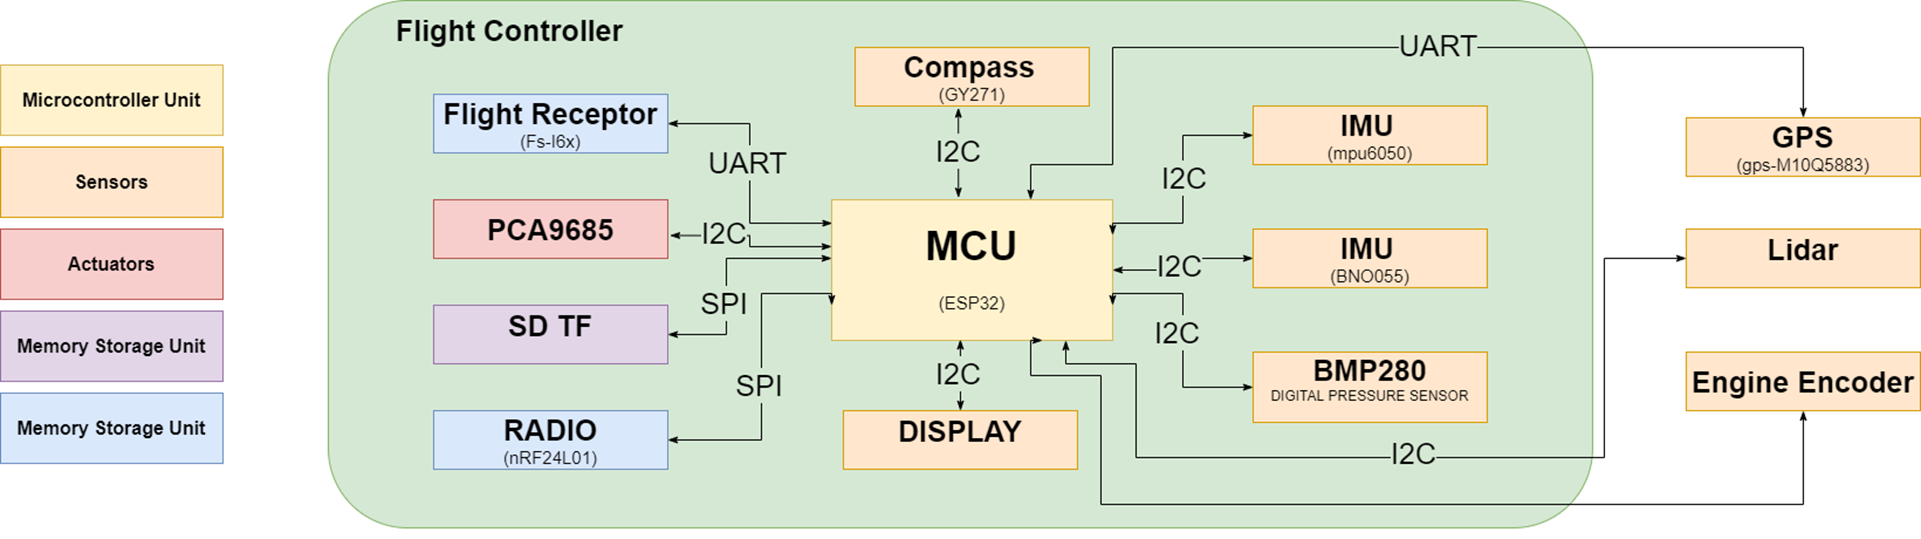
\includegraphics[width=\textwidth]{Imagenes/Metodologia/arquitectura_controlador.png}
    \caption{Arquitectura del controlador de vuelo diagrama de Caja Gris }
    \label{fig:arqui_controlador}
\end{figure}

Para ver de forma más detallada como sería esta arquitectura y como se integraría con los distintos módulos, se desarrollo el siguiente diagrama de Caja Blanca (véase \ref{fig:arqui_Blanxa}) , en el que se puede observar con más detalle cuales serán los componentes principales en la estructura del dispositivo. De este diagrama todos los dispositivos que están encapsulados por el recuadro verde, indican que están inmersos en el sistema mientras que todos los que se encuentran por fuera son módulos adicionales o que se encuentran en otra parte del Sistema.

\begin{figure}[H]
    \centering
    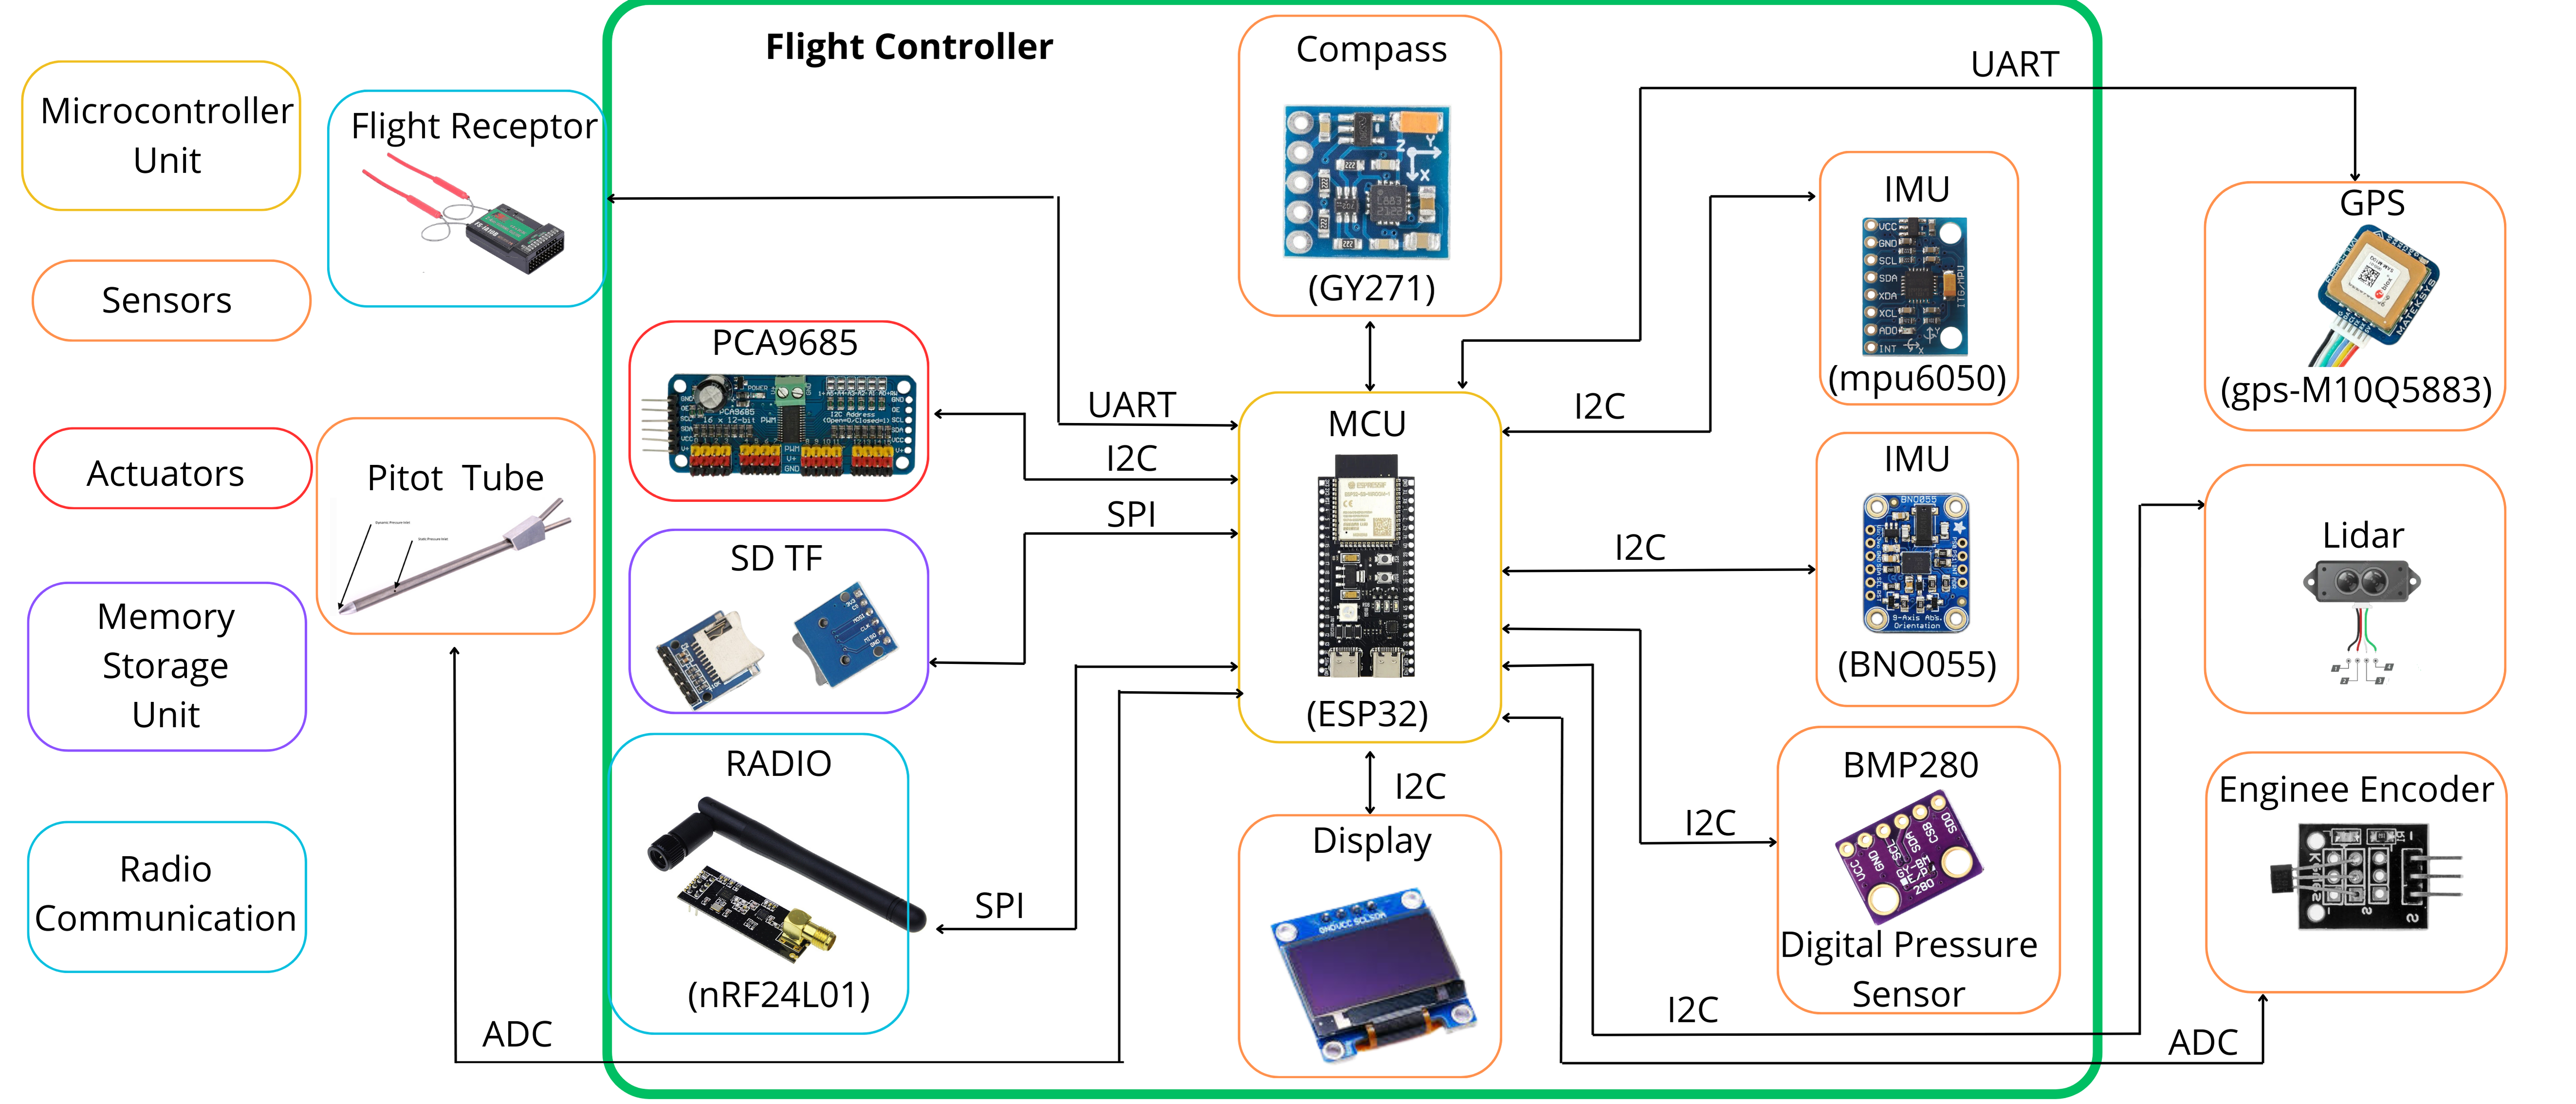
\includegraphics[width=\textwidth]{Imagenes/Metodologia/arquitecturaModulos.png}
    \caption{Arquitectura del controlador de vuelo diagrama de Caja Blanca }
    \label{fig:arqui_Blanxa}
\end{figure}

\subsection{Circuito Impreso}
Una vez finalizada la etapa de diseño y habiendo terminado de definir los componentes que conformaran el sistema, se procede a diseñar un circuito impreso \textbf{PCB}. A lo largo de este proyecto se realizaron en total 2 iteraciones del circuito para mejorar la estabilidad y eficiencia del circuito. El primer circuito fabricado se puede observar en \ref{fig:sch-1.0}, \ref{fig:pcb-1.0} y \ref{fig:pcb-ensambled-1.0}. Para esta primera iteración se utilizó como \textbf{MCU} un \textbf{ESP32 DevKit v1}, el cual presentaba ciertas deficiencias relacionadas con el protocolo I2C. En esta versión, el módulo \textbf{PCA9685} tenía un voltaje de alimentación lógico de \textbf{5V}, mientras que todos los demás voltajes de alimentación de los módulos de I2C se encontraban alimentados con \textbf{3.3V}. Esto generaba errores con los buses de \textbf{SDA} y \textbf{SCL}. Este error se puede abordar de dos formas. Agregando resistencias de \textbf{Pull-Up} de \textbf{4.7 k$\Omega$}, o alimentando toda la parte lógica a \textbf{3.3V}. Se decidió optar por la segunda opción. \\ \\
    


Otro problema relacionado con la \textbf{PCA9685} fue el de alimentación del pin \textbf{V+} o el voltaje de entrada del módulo. Puesto que inicialmente se tenía este dispositivo alimentado a una tensión de \textbf{+5v}, la cual al momento de realizar pruebas de movimiento de los servomotores generaba un consumo elevado de corriente que causaba un overshoot de voltaje y ocacionaba un reset en el dispositivo. 


\subsubsection{ Diseño del Esquemático Final}\\ \\

El software donde se diseñaron las dos versiones del circuito fue \textbf{KIcad} versión \textbf{8.0}. Este software fue seleccionado, puesto que es \textbf{Open Source} y hay un gran número de huellas y componentes creados por la comunidad. \\

Para el apartado de diseño del circuito impreso se hace necesario diseñar el esquemático a seguir, el cual consiste en la selección y asociación de \textbf{símbolos} y \textbf{huellas} con el ruteo eléctrico de todos y cada uno de los componentes del sistema. \\


El esquemático se dividió en varias partes (véase \ref{fig:sch2.0}), en este apartado tenemos 7 secciones principales. La primera de ellas localizada en la parte superior izquierda llamada \textbf{ESP32-S3} que muestra todas las conexiones relacionadas con el MCU. Seguidamente se observa el apartado de \textbf{SPI}, en el que se encuentran los distintos módulos configurados bajo este protocolo, los cuales son el \textbf{micro SD-CARD Module}, seguido del módulo transmisor \textbf{NRF24L1}. En la parte superior derecha se muestra el apartado de \textbf{UART} en el que se tiene la posibilidad de tener 2 dispositivos bajo este protocolo, el \textbf{GPS} y otro adicional que se requiera. En la mitad se tienen 2 secciones dedicadas a los \textbf{sensores} y módulos \textbf{I2C}. En la parte inferior derecha está el apartado dedicado al \textbf{Power Suply} que es la etapa encargada de gestionar la alimentación del dispositivo. En esta etapa se resalta el hecho de que la entrada debe ser de una batería externa de \textbf{7.4 v} y regula a una salida de \textbf{5V} para todo el sistema. Finalmente, en la parte inferior derecha se tiene el \textbf{FS-I6X} el cual corresponde a los pines donde se va a conectar el receptor externo \textbf{Flysky}. \\

Cabe resaltar que se crearon 2 footprints para el dispositivo. El de los módulos de la \textbf{PCA9585} y el del \textbf{BNO055} los cuales se realizaron en base a la documentación oficial de estos módulos obtenidos directamente de la tienda \textbf{Adafruit Learning System}
\\ \\
\begin{figure}[H]
    \centering
    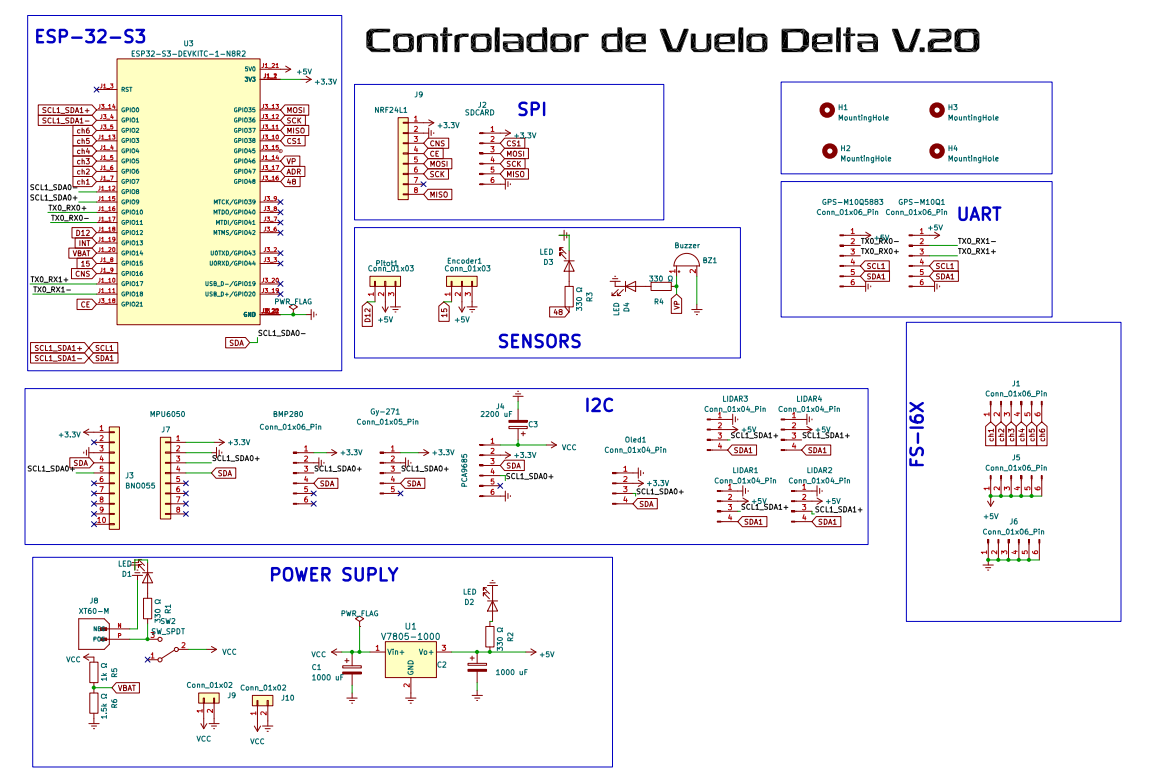
\includegraphics[width=\textwidth]{Imagenes/Metodologia/SCH2.0.png}
    \caption{Esquematico Circuito Impreso 2.0 }
    \label{fig:sch2.0}
\end{figure}

\subsubsection{Diseño del Layout del PCB final} \\ \\

El \textbf{PCB} fue diseñado en dos capas (véase \ref{fig:pcb_2.0} ). En la capa \textbf{TOP} se realizaron varios planos relacionados  con los distintos voltajes de operación del dispositivo, en los que encontramos el de alimentación por batería externa de \textbf{7.4 v}  resaltado en color verde , seguidamente del plano resaltado con color amarillo de \textbf{3.3 v} y finalmente el de \textbf{5v} que serían los planos restantes de \textbf{5V}. En la capa de \textbf{Bottom} se hicieron solamente 2 planos, el de \textbf{7.4 v} resaltado de verde y el de \textbf{GND} que es de color \textbf{azul} en el que se encuentran todas las tierras generales del dispositivo. \\
\begin{figure}[H]
    \centering
    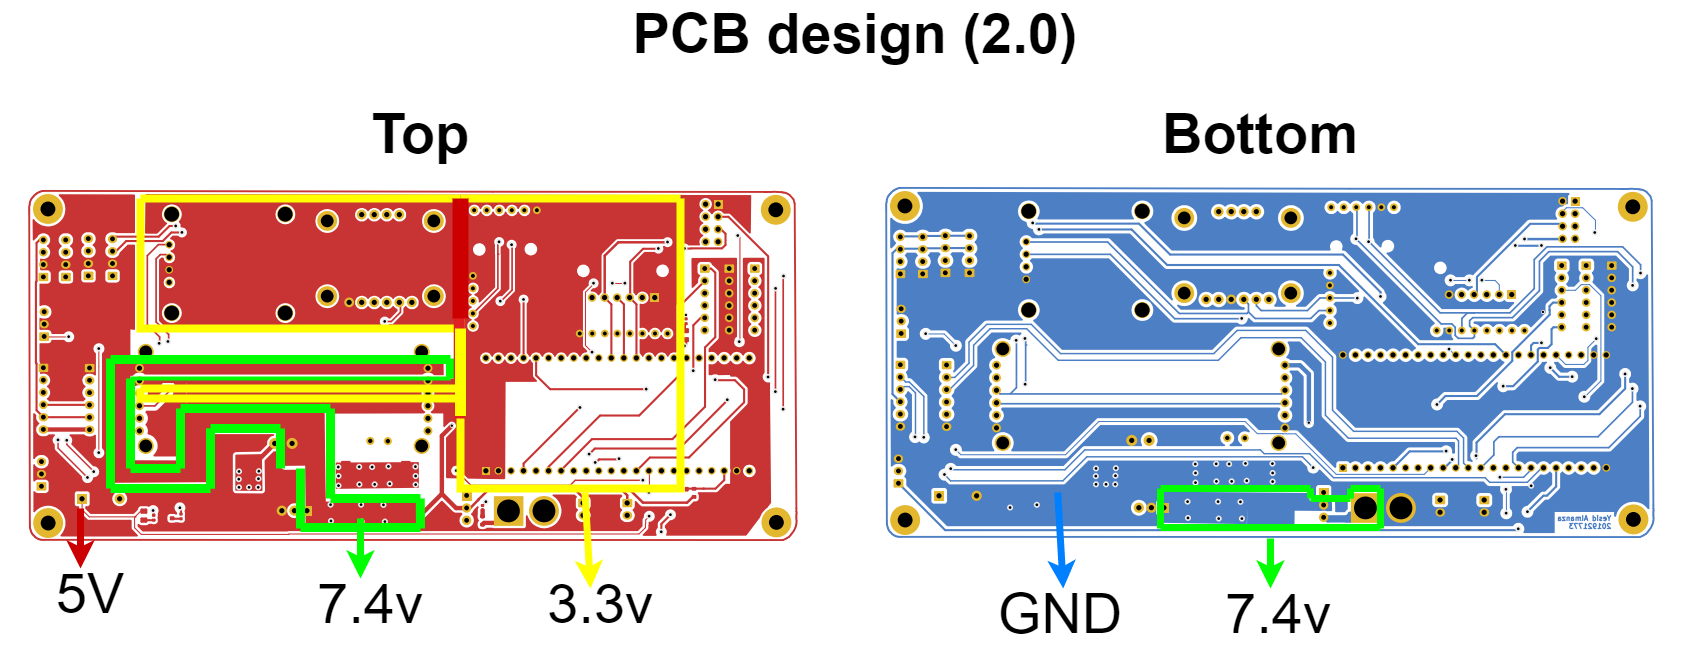
\includegraphics[width=\textwidth]{Imagenes/Metodologia/PCB20.png}
    \caption{Layout Circuito Impreso 2.0 }
    \label{fig:pcb_2.0}
\end{figure}

\\
Para el diseño del layout de la PCB se tuvo en consideración la normativa IPC 2221, la cual establece estándares esenciales para el diseño de placas de circuitos impresos. En la Figura \ref{fig:ipc2221}, se muestran los parámetros clave de esta normativa, incluyendo el ancho de pista, el ancho de separación y la distribución de componentes. Estas directrices aseguran un diseño robusto y seguro, considerando aspectos como la corriente que pueden soportar las pistas, las distancias de separación necesarias según el voltaje, y una distribución eficiente de los componentes para minimizar interferencias y optimizar el rendimiento del circuito.\cite{IPC} \\

\begin{figure}[H]
    \centering
    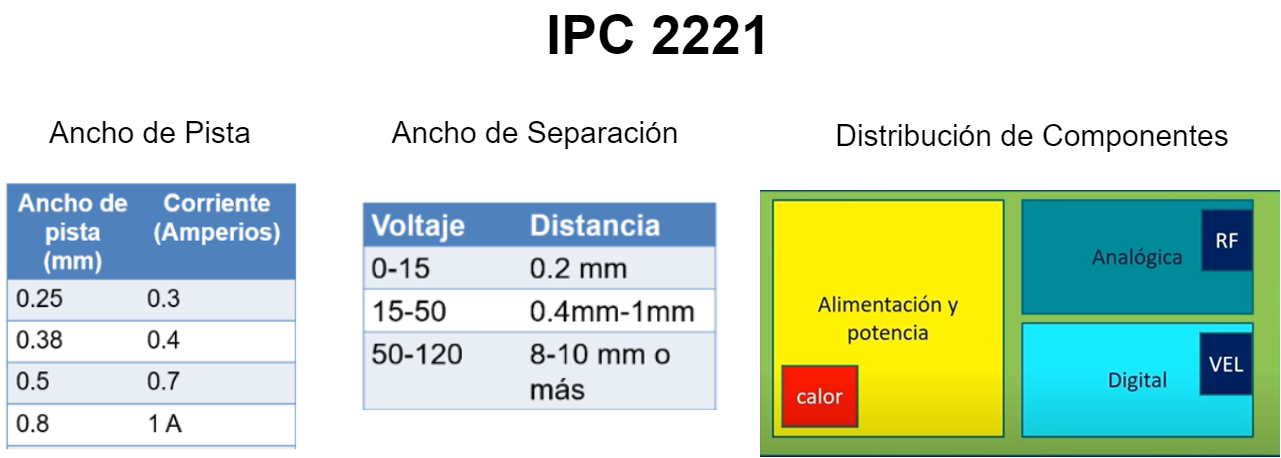
\includegraphics[width=\textwidth]{Imagenes/Metodologia/ipc2221.png}
    \caption{Normativa IPC 2221 \cite{IPC} }
    \label{fig:ipc2221}
\end{figure}

\\
Una vez finalizado el apartado de diseño del layout se procedió a buscar los distintos modelos 3d de los distintos componentes para poder situarlos en un ensamble y observar las dimensiones finales del circuito impreso con los distintos módulos. El tamaño final del \textbf{pcb} fue de \textbf{71.5 mm} de ancho, \textbf{156 mm} de largo \textbf{21.6 mm} de alto. La distribución de los componentes se puede ver a continuación. 
\begin{figure}[H]
    \centering
    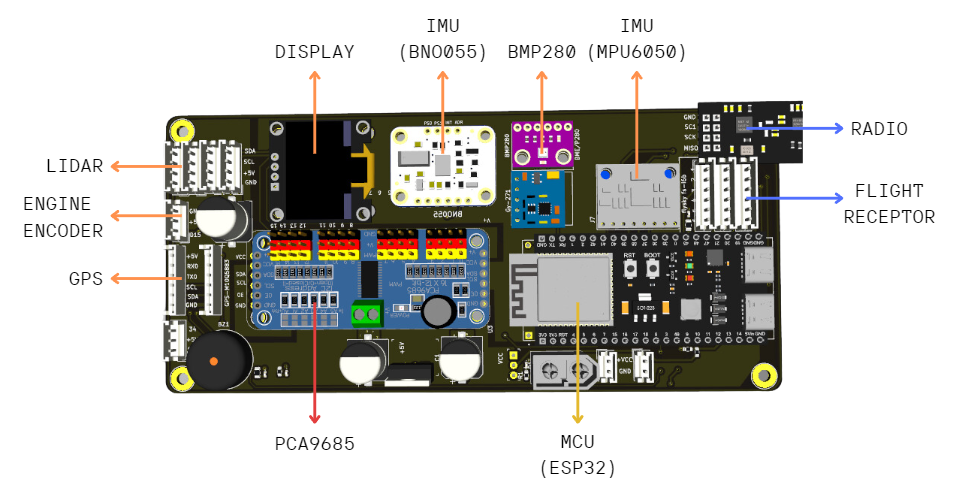
\includegraphics[width=\textwidth]{Imagenes/Metodologia/model3d.png}
    \caption{Modelo 3d Circuito Impreso}
    \label{fig:model3d_pcb}
\end{figure}

\\ \\
\subsubsection{Fabricación del PCB}
\\ \\
El \textbf{Printed Circuit Board (PCB)} fue fabricado en el laboratorio de circuitos impresos de la Universidad de los Andes. Se fabricaron tres de los mismos circuitos en caso de que hubiera algún fallo con alguno de los PCBs. Estos PCBs se fabricaron usando un sustrato de FR4, conocido por su excelente estabilidad térmica y propiedades dieléctricas. Además, el PCB cuenta con tecnología True Hole, lo que garantiza la continuidad eléctrica entre capas.

\\
Para asegurar la calidad y fiabilidad, la fabricación siguió el estándar IPC de fabricación de circuitos impresos, garantizando que el PCB cumple con los requisitos estándares de calidad y rendimiento.
\\

\subsubsection{ Montaje del PCB}
\\ \\

La PCB fue ensamblada teniendo en cuenta los grupos de componentes en ambas capas. Todos los módulos están en la capa superior a excepción del módulo de lectura SD que se encuentra en la capa inferior. Se tomó esta decisión en particular para ahorrar espacio y mejorar la accesibilidad a los componentes significativos durante el mantenimiento y el ensamblaje.

\\ \\

La mayoría de los módulos fueron conectados a través de regletas de inserción, para que en caso de fallo o actualización, los componentes respectivos puedan ser reemplazados sin esfuerzo. Sin embargo, en el módulo SD de lectura, las regletas de inserción no fueron preferidas, ya que estas pueden causar una mala unión mecánica que lleva a la inestabilidad del sistema. La Figura \ref{fig:ensamblada} es una imagen de la tarjeta ensamblada, de la que se puede ver claramente la disposición de los diferentes módulos en la tarjeta. La disposición se ha planeado de tal manera que proporciona un ensamblaje fuerte y adecuado con respecto a las necesidades funcionales y de mantenimiento del equipo.

\begin{figure}[H]
    \centering
    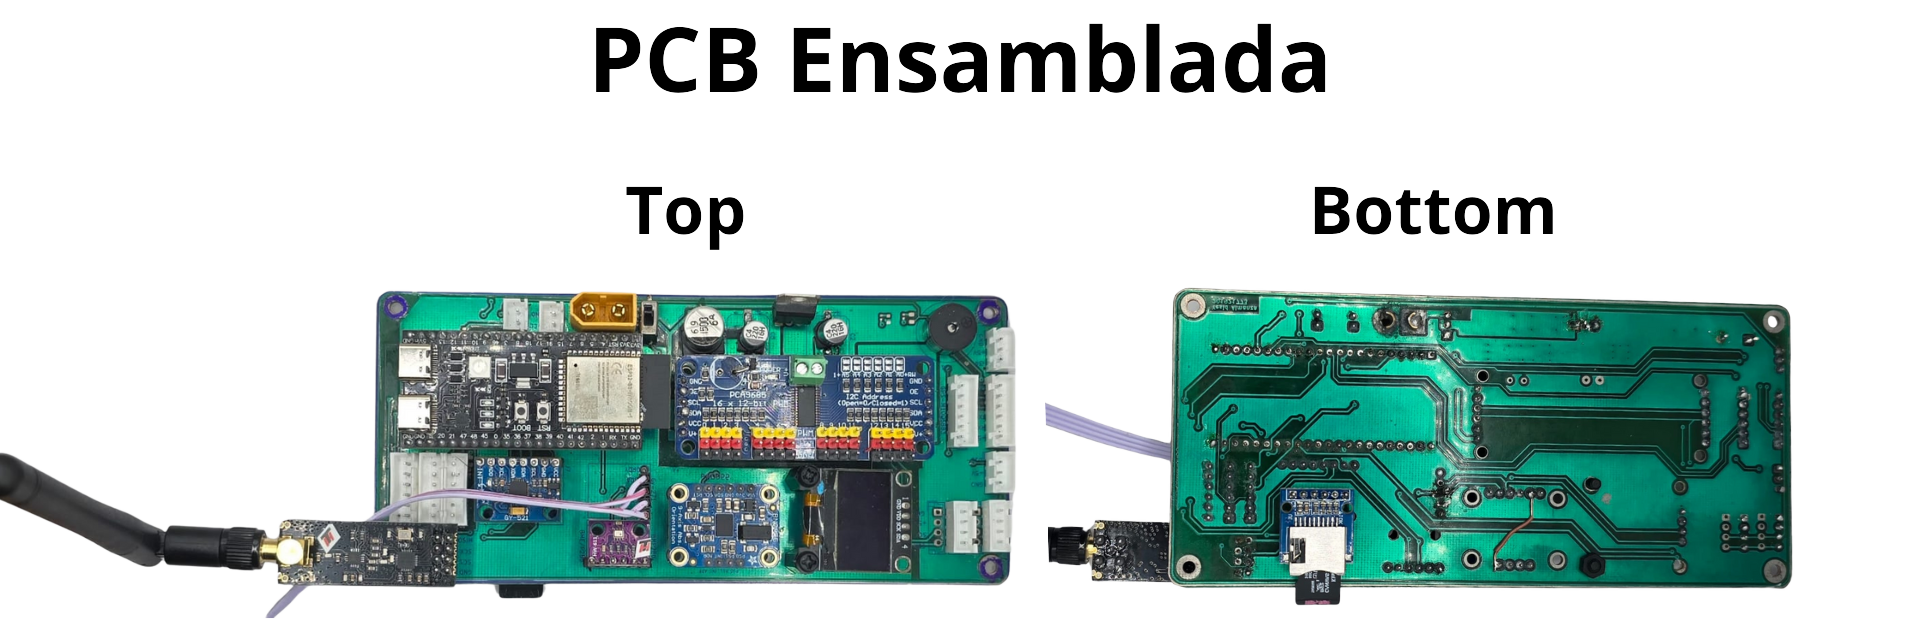
\includegraphics[width=\textwidth]{Imagenes/Metodologia/pcb_ensamblada.png}
    \caption{PCB ensamblada}
    \label{fig:ensamblada}
\end{figure}
\vspace{5 px}\\ \\
\clearpage
%\input{Sections/Enclosure}
\clearpage 
%\section{Desarrollo de Firmware}


El desarrollo del firmware se abordó desde varios puntos que se trabajaron en paralelo para garantizar su correcto funcionamiento. El firmware desarrollado fue estructurado considerando que el lenguaje de programación utilizado es C++, optando por la filosofía de programación orientada a objetos. Por lo tanto, se implementaron clases independientes para los diferentes módulos del sistema, como Sensórica, Control y el Receptor FlySky. Estas clases son gestionadas desde el programa principal (main), asegurando una organización modular y facilitando el mantenimiento y la escalabilidad del código. Esta metodología permite una interacción clara y definida entre los distintos componentes del sistema, asegurando que cada módulo funcione de manera autónoma pero coordinada dentro del controlador de vuelo del UAV.

\subsection{Entorno de Programación}

El firmware desarrollado para el controlador de vuelo fue escrito en C++ utilizando el framework de \textbf{Espressif}. Para el desarrollo y gestión del proyecto se empleó PlatformIO, una herramienta multiplataforma que permite programar en diferentes boards de manera eficiente y flexible. El entorno de programación utilizado fue Visual Studio Code, que ofrece una interfaz amigable y numerosas extensiones útiles para el desarrollo de proyectos embebidos. \\ \\

Inicialmente, el proyecto fue diseñado y programado para una board ESP32. Posteriormente, se migró a una ESP32-S3, una versión más reciente y avanzada de este microcontrolador. Esta migración se realizó para aprovechar las mejoras y características adicionales que ofrece la ESP32-S3, asegurando un rendimiento superior y una mayor capacidad de procesamiento para las tareas del controlador de vuelo.

\begin{comment}
    

\section{ESP32-S3}
El núcleo del sistema o \textbf{MCU} es el microcontrolador ESP32-S3 de Espressif, un System on ChipSoC (SoC) que integra funcionalidades avanzadas de Wi-Fi y Bluetooth LE, optimizado para aplicaciones de bajo consumo energético y alta eficiencia en la comunicación. Facilita la integración con una amplia variedad de sensores y actuadores a través de interfaces periféricas, utilizando protocolos estándar de la industria como I2C, UART y SPI.\cite{ESP32S3}

\vspace{10 px}
\subsection{\textbf{Descripción del Pinout del ESP32-S3}}
El pinout del ESP32-S3 es crucial para la interfaz con diversos sensores y actuadores en el controlador de vuelo. A continuación, se describen algunos pines específicos y su funcionalidad dentro del sistema: 

\begin{figure}[H]
    \centering
    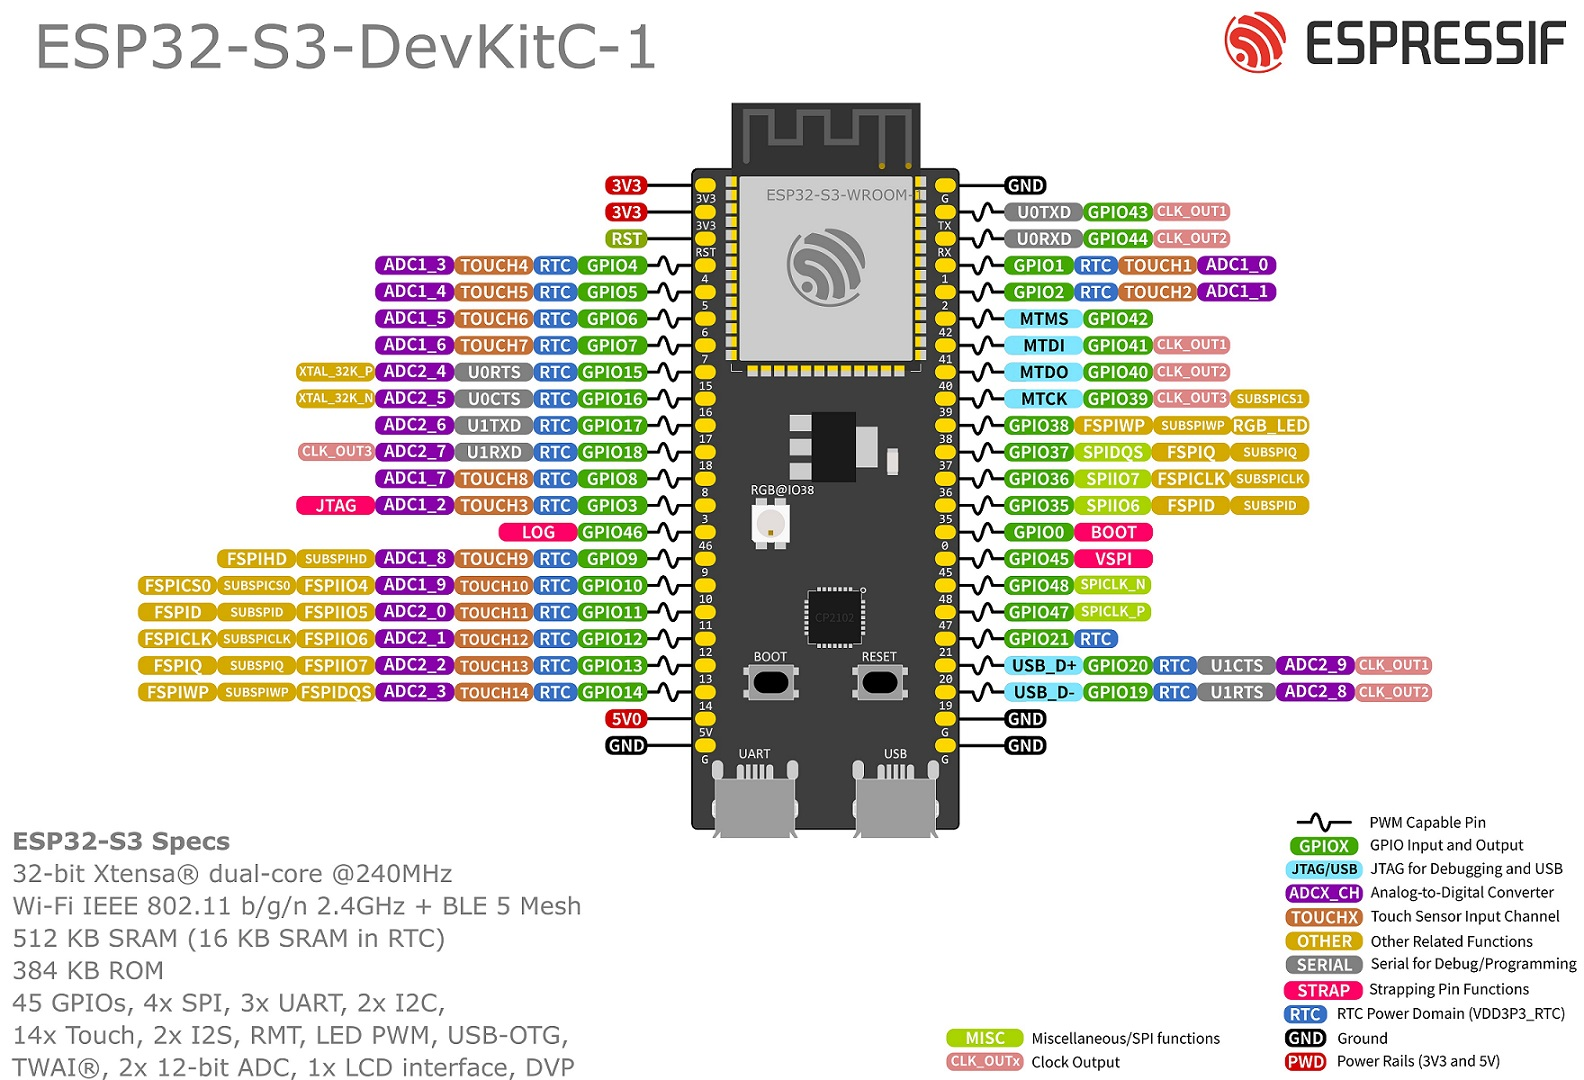
\includegraphics[width=6 in]{Imagenes/Metodologia/ESP32-S3_DevKitC-1_pinlayout_v1.1.jpg}
    \caption{Pinout del ESP32-S3 \cite{ESP32S3}}
    \label{fig:arqui_controlador}
\end{figure}





\paragraph{\textbf{Pines de Comunicación Serial (UART)}}
\begin{itemize}
    \item \textbf{GPIO1 (U0TXD)} y \textbf{GPIO3 (U0RXD)}: Estos pines son utilizados para la comunicación UART, esencial para la transmisión de datos hacia y desde el módulo GPS. La capacidad de comunicación bidireccional es fundamental para recibir datos de ubicación y enviar configuraciones al GPS.
    \item \textbf{GPIO17 (U1TXD)} y \textbf{GPIO18 (U1RXD)}: Pines alternativos para comunicación UART, utilizados para conectar dispositivos adicionales que requieran comunicación serial.\cite{ESP32S3}
\end{itemize}

\paragraph{\textbf{Pines I2C}}
\begin{itemize}
    \item \textbf{GPIO5 (SCL)} y \textbf{GPIO4 (SDA)}: Estos pines facilitan la comunicación I2C, usados principalmente para interconectar sensores como el BMP280 (sensor de presión) y el IMU. Permiten la transmisión de comandos y la recepción de datos del sensor de manera eficiente.\cite{ESP32S3}
\end{itemize}

\paragraph{\textbf{Pines de Alimentación y Control}}
\begin{itemize}
    \item \textbf{3V3 y GND}: Pines de alimentación que proveen la energía necesaria para el funcionamiento del ESP32-S3 y los periféricos conectados. Es crucial asegurar una conexión estable y de adecuada capacidad de corriente para evitar reinicios inesperados o malfuncionamiento del hardware.
    \item \textbf{EN (Enable)}: Pin utilizado para habilitar o reiniciar el microcontrolador. Un pulso bajo en este pin puede reiniciar el sistema, lo cual es útil durante el desarrollo y en situaciones de error en campo.
\end{itemize}

\paragraph{\textbf{Pines de Propósito General (GPIO)}}
\begin{itemize}
    \item \textbf{GPIO21, GPIO22, GPIO23}: Pines configurables para entrada o salida general, utilizados en este proyecto para controlar LEDs indicadores de estado, actuadores o leer señales de sensores adicionales.
\end{itemize}

\paragraph{Pines Especiales}
\begin{itemize}
    \item \textbf{GPIO0 (BOOT)}: Utilizado para entrar en el modo de programación del ESP32-S3 al inicio. Debe estar en bajo durante el reinicio para activar la carga de nuevos programas, lo que es esencial durante las fases de desarrollo y prueba.
\end{itemize}

Esta configuración de pines permite la interacción entre el microcontrolador y los distintos componentes del sistema de control de vuelo, asegurando la operatividad y la eficiencia en la gestión de los recursos y tareas asignadas.
\\ \\
\subsection{Hardware Serial}
ESP32-S3 soporta múltiples canales UART, lo que permite una comunicación serial robusta y flexible. Esta capacidad es esencial para el intercambio de datos en tiempo real entre el controlador de vuelo y otros componentes del sistema, como módulos GPS y sensores IMU, garantizando una transmisión de datos eficiente y confiable.
\\ \\
\subsection{Modo de arranque}
El modo de arranque del ESP32-S3 se configura mediante el estado de varios pines de arranque durante el reset del dispositivo. Esto proporciona una flexibilidad significativa para la carga de diferentes programas y el desarrollo de software, permitiendo que el dispositivo se adapte a diversas aplicaciones y escenarios de uso. El modo de arranque puede influir en cómo el dispositivo gestiona la seguridad del arranque y la integridad del firmware.
\\
\subsection{Carga de programa}
La carga de programas en el ESP32-S3 se realiza a través de interfaces estándar como UART o mediante el puerto USB. El entorno de desarrollo proporciona herramientas que facilitan la escritura, el debug y la carga de software, soportando lenguajes como C y Python. Esto permite a los desarrolladores programar el dispositivo con facilidad, implementar actualizaciones de firmware y realizar mantenimiento en campo.\\ \\

\subsection{Procesador y memoria}
\paragraph{\textbf{Procesador de doble núcleo}}
El procesador de \textbf{doble núcleo del ESP32-S3} opera a una frecuencia de hasta \textbf{240 MHz}, proporcionando una capacidad de procesamiento considerable para tareas múltiples y simultáneas. Esta característica es crítica para aplicaciones que requieren respuestas rápidas y procesamiento en tiempo real, como el control de vuelo en UAVs. \cite{ESP32S3}\\

\paragraph{\textbf{Memoria interna}}
El ESP32-S3 está equipado con memoria interna suficiente para gestionar las operaciones del sistema y el almacenamiento temporal de datos. La memoria interna se divide en varios bloques, incluyendo ROM para el arranque y firmware básico, y SRAM para la ejecución de programas y almacenamiento de variables durante la operación.cite{ESP32S3}\\

\paragraph{\textbf{Memoria externa}}
El microcontrolador soporta memoria externa a través de interfaces SPI, permitiendo la expansión del almacenamiento para aplicaciones que acumulan grandes volúmenes de datos, como registros de vuelo o datos sensoriales. La flexibilidad en la gestión de la memoria externa facilita la implementación de sistemas complejos y la adaptación a requerimientos específicos de almacenamiento y procesamiento.\cite{ESP32S3}\\

%end{comment}

\subsection{Verificación de Conectividad Sensores y Actuadores }
Antes de proceder con la sensórica, es fundamental realizar una verificación de los sensores y actuadores conectados al sistema. Este paso incluye un escaneo de las direcciones de los dispositivos I2C, asegurando que todos los componentes estén correctamente conectados al bus I2C. Este escaneo permite identificar qué dispositivos están presentes y si falta alguno, lo que facilita la detección de problemas de conexión antes de inicializar el programa.\\ \\

\\ \\
\subsubsection{Escaneo de direcciones I2C} \\ \\

Para determinar el correcto funcionamiento del bus I2C, se diseñó un software que detecta los dispositivos conectados al bus y cuántos hay. Este procedimiento se ejecuta cada vez que se inicia el dispositivo. A continuación, se presentan los resultados del escaneo de direcciones I2C:\\ \\

\begin{figure}[H]
    \centering
    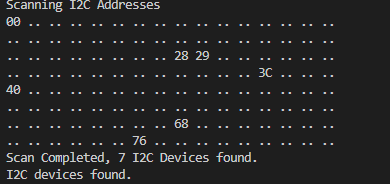
\includegraphics[width=10 cm]{Imagenes/Metodologia/I2C_scan.png}
    \caption{Escaneo I2C de los dispositivos conectados.}
    \label{fig:i2c_scan}
\end{figure}

Los dispositivos detectados en el bus I2C y sus correspondientes direcciones son:\\ \\

\begin{itemize}
    \item \textbf{0x28}: Corresponde al tubo de Pitot.
    \item \textbf{0x29}: Corresponde al sensor de orientación \textbf{BNO055}.
    \item \textbf{0x40}: Corresponde al controlador de servos PCA9685.
    \item \textbf{0x76}: Corresponde al sensor de presión barométrica BMP280.
    \item \textbf{0x68}: Corresponde al acelerómetro y giroscopio \textbf{MPU6050}.
    \item \textbf{0x00}: Corresponde a la pantalla OLED.
\end{itemize}\\ \\





\subsection{Sensorica y adquisición de datos} \\ \\

    Los sensores son uno de los componentes más críticos en el controlador de vuelo, proporcionando los datos necesarios para la navegación y el control de estabilidad del UAV. Estos incluyen dos Unidades de Medición Inerciales \textbf{IMUs} para la detección de movimiento y orientación de la aeronave, un \textbf{barómetro} para medir la presión atmosférica y la altura de la aeronave. Finalmente un módulo \textbf{GPS} para obtener la posición geográfica de la aeronave en todo momento. \\ \\


\subsubsection{ Unidades de Medición Inerciales} \\ \\


    En el tema de las Unidades de Medición Inerciales IMUs se selecciono como IMU principal al \textbf{BNO055} debido a que es un sensor de alta precisión que integra acelerómetro, giroscopio, magnetómetro y un procesador ARM Cortex-M0 para el cálculo en tiempo real de la orientación y movimiento, ofreciendo datos fiables y precisos con una frecuencia de actualización de hasta 100 Hz \cite{IMU}. En contraste, el \textbf{MPU6050}, aunque menos avanzado, es una opción económica que proporciona seis grados de libertad y capacidades decentes para la medición de movimiento y orientación gracias a su giroscopio y acelerómetro integrados. Se comunican ambos a través del protocolo de comunicación I2C y se puede programar para diferentes sensibilidades.\cite{BNO} \\ 
    
    
    
    En caso de que se produzca un fallo con el \textbf{BNO055}, el \textbf{MPU6050} serviría como un sistema de respaldo eficiente. Aunque no ofrece la misma precisión y el conjunto de características que el \textbf{BNO055}, su capacidad para proporcionar seguimiento de movimiento y datos de inclinación lo convierte en un sustituto confiable que puede mantener la funcionalidad del sistema hasta cierto nivel hasta que se resuelva el problema principal. \\ 

    La comparación entre las especificaciones del sensor \textbf{BNO055} y el sensor \textbf{MPU6050} revela diferencias significativas en sus capacidades de procesamiento de datos y aplicaciones. El \textbf{BNO055}, como se detalla en el Cuadro \ref{tab:bno055_specs}, ofrece cálculos internos que proporcionan la orientación del dispositivo en diferentes formatos, incluidos grados, radianes y cuaterniones. Esto significa que el \textbf{BNO055} entrega directamente datos de orientación tridimensional, vector de velocidad angular, vector de aceleración, vector de fuerza del campo magnético y temperatura, sin necesidad de procesamiento adicional. Este enfoque integrado facilita su uso en aplicaciones donde se requiere una rápida interpretación y utilización de los datos de movimiento.  \\ 
    
    Por otro lado, el sensor \textbf{MPU6050}, según el Cuadro \ref{tab:mpu6050_specs}, requiere un postprocesamiento de la aceleración angular en cada uno de los ejes del dispositivo para obtener la orientación. Mientras que el \textbf{MPU6050} proporciona datos de giroscopio y acelerómetro en bruto, junto con soporte para filtros y funciones programables, el cálculo de la orientación en grados, radianes o cuaterniones debe realizarse externamente. Esto implica un esfuerzo adicional en el procesamiento de datos para lograr el mismo nivel de interpretación inmediata que ofrece el \textbf{BNO055}. \\ 
    
    En resumen, mientras que el \textbf{BNO055} simplifica la integración y el uso con su capacidad de cálculo interno de orientación, el \textbf{MPU6050} requiere un procesamiento posterior de los datos para obtener resultados similares, lo que puede ser una consideración importante en el diseño y la implementación de sistemas que dependen de la precisión y rapidez de los datos de orientación.

    
\paragraph{\textbf{\textbf{BNO055}}}

    \begin{table}[h]
\centering
\caption{Especificaciones del Sensor \textbf{BNO055}}
\label{tab:bno055_specs}
\begin{tabular}{|l|l|}
\hline
\textbf{Característica} & \textbf{Descripción} \\ \hline
Orientación Absoluta (Vector Euler, 100Hz) & Datos de orientación tridimensional basados en una esfera de 360° \\ \hline
Orientación Absoluta (Quaternión, 100Hz) & Salida de cuaternión de cuatro puntos para manipulación precisa de datos \\ \hline
Vector de Velocidad Angular (100Hz) & Tres ejes de 'velocidad de rotación' en rad/s \\ \hline
Vector de Aceleración (100Hz) & Tres ejes de aceleración (gravedad + movimiento lineal) en m/s\textsuperscript{2} \\ \hline
Vector de Fuerza del Campo Magnético (20Hz) & Tres ejes de detección de campo magnético en micro Tesla (uT) \\ \hline
Vector de Aceleración Lineal (100Hz) & Tres ejes de datos de aceleración lineal (aceleración menos gravedad) en m/s\textsuperscript{2} \\ \hline
Vector de Gravedad (100Hz) & Tres ejes de aceleración gravitacional (menos cualquier movimiento) en m/s\textsuperscript{2} \\ \hline
Temperatura (1Hz) & Temperatura ambiente en grados Celsius \\ \hline
\end{tabular}
\end{table}

\begin{table}[H]
\centering
\caption{Especificaciones del Sensor \textbf{MPU6050}}
\label{tab:mpu6050_specs}
\begin{tabular}{|l|l|}
\hline
\textbf{Característica} & \textbf{Descripción} \\ \hline
Giroscopio & Salida digital en ejes X, Y, Z con escalas de ±250, ±500, ±1000, y ±2000°/sec \\ \hline
Acelerómetro & Salida digital de 3 ejes con escalas de ±2g, ±4g, ±8g, y ±16g \\ \hline
Voltaje de Trabajo & 2.375-3.46V \\ \hline
Voltaje de Lógica I2C & 1.71V a VDD \\ \hline
Interface Serial & I2C \\ \hline
ADC & 16 bits para giroscopio y acelerómetro \\ \hline
Procesador de Movimiento & DMP integrado para procesamiento de movimiento en 3D y algoritmo de reconocimiento de gestos \\ \hline
Filtros & Filtros pasa bajo programables \\ \hline
Interrupciones Programables & Soporta funciones como reconocimiento de gestos, detección de golpe y movimiento \\ \hline
\end{tabular}
\end{table}
\\ \\
\paragraph{\large \textbf{ Marcos de Referencia para la Medición de Ángulos en el Controlador de Vuelo}} \\ \\

Inicialmente, se estableció el marco de referencia de los ángulos que va a medir el controlador con respecto al marco de referencia del UAV. Los ejes ilustrados representan las orientaciones críticas: yaw (giro alrededor del eje vertical), pitch (inclinación hacia adelante o hacia atrás) y roll (rotación sobre el eje longitudinal) \ref{fig:movimientos_inerciales}. Estos ángulos son fundamentales para el control de la orientación del UAV, y el controlador de vuelo está diseñado para recopilar y procesar datos sobre cada uno de estos ejes, permitiendo así ajustes precisos en tiempo real para mantener la estabilidad del dispositivo.

\begin{figure}[H]
    \centering
    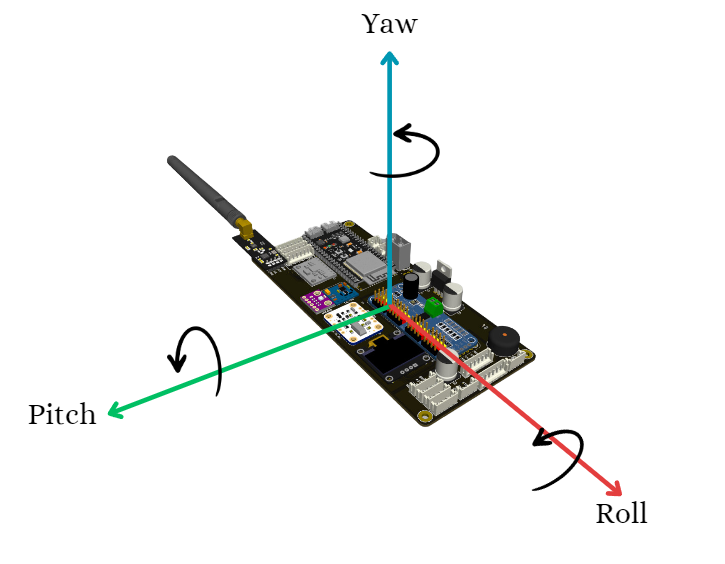
\includegraphics[width=0.8\textwidth]{Imagenes/Metodologia/pcb_yaw_pitch_roll.png}
    \caption{Movimientos Inerciales Yaw, Pitch y Roll en el controlador de vuelo}
    \label{fig:movimientos_inerciales}
\end{figure}
\\ \\
\paragraph{\large \textbf{Filtrado y recopilación de datos de movimientos inerciales}}
\\ \\

Para este apartado, se leyeron y procesaron datos tomados del sensor \textbf{MPU6050}. Se realizó un algoritmo en el que se aplican filtros de Kalman para estimar los ángulos de orientación del dispositivo (Roll, Pitch, Yaw) a partir de las mediciones del sensor. Esto con el objetivo de mejorar la precisión de estas estimaciones al reducir el ruido y combinar de manera óptima ambas fuentes de datos. \\ 

El filtro de Kalman es un enfoque matemático que se utiliza ampliamente en aplicaciones de control y navegación para estimar el estado de sistemas dinámicos a partir de mediciones ruidosas. Este algoritmo se basa en dos fases principales: predicción y actualización. Estas se utilizan iterativamente para mejorar la estimación del estado del sistema con cada nueva medición.
\\ \\
\subparagraph{\textbf{\large Fase de Predicción}} \\ \\

En la fase de predicción, el filtro de Kalman utiliza un modelo del sistema para predecir el próximo estado, basándose en el estado estimado actual y en el conocimiento de cómo evoluciona el sistema con el tiempo. Esta predicción también incluye una estimación de la incertidumbre (o error) asociada con el estado predicho. La incertidumbre se modela como una matriz de covarianza, que cuantifica la confianza en la predicción del estado. Para esto se tiene que: \\

\[
\hat{x}_{k|k-1} = A\hat{x}_{k-1|k-1} + B u_k
\]
\[
P_{k|k-1} = A P_{k-1|k-1} A^T + Q
\]
\\
En donde:

\\
\begin{itemize}
    \item $\hat{x}_{k|k-1}$ es la estimación del estado en el tiempo $k$, dada la información hasta el tiempo $k-1$.
    \item $A$ es la matriz del modelo de transición del estado.
    \item $\hat{x}_{k-1|k-1}$ es la estimación del estado en el tiempo $k-1$, dada toda la información hasta el tiempo $k-1$.
    \item $B$ es la matriz del modelo de control.
    \item $u_k$ es el vector de control en el tiempo $k$.
    \item $P_{k|k-1}$ es la covarianza del error de predicción en el tiempo $k$.
    \item $Q$ es la covarianza del ruido del proceso.
\end{itemize}
\\ \\
En esta fase de predicción, se actualizará el ángulo de Roll basado en la velocidad angular previa, ajustada por el sesgo estimado, y el paso de tiempo. Además, se actualizan las matrices de covarianza de error para reflejar la nueva incertidumbre después de la predicción.

\subparagraph{\textbf{\large Fase de Actualización}}

En la fase de actualización, se ajusta la estimación del estado con base en la nueva medición:

\[
K_k = P_{k|k-1} H^T (H P_{k|k-1} H^T + R)^{-1}
\]
\[
\hat{x}_{k|k} = \hat{x}_{k|k-1} + K_k (z_k - H \hat{x}_{k|k-1})
\]
\[
P_{k|k} = (I - K_k H) P_{k|k-1}
\]

En donde:
\begin{itemize}
    \item $K_k$ es la ganancia de Kalman en el tiempo $k$.
    \item $H$ es la matriz del modelo de observación.
    \item $R$ es la covarianza del ruido de observación.
    \item $z_k$ es la medición real en el tiempo $k$.
    \item $I$ es la matriz identidad, con dimensiones adecuadas para la operación.
\end{itemize}
\\ \\
En esta fase de actualización, se calcula la discrepancia entre la estimación del ángulo a partir del acelerómetro y la predicción del ángulo de Roll. Además, se calculan las ganancias de Kalman, que determinan cómo se combinan la predicción y la medición para obtener una nueva estimación. Por otro lado, se actualizan el ángulo estimado de Roll y el sesgo utilizando las ganancias de Kalman. Por último, se ajustan las matrices de covarianza de error para reflejar la disminución en la incertidumbre después de la actualización. \\

Estas ecuaciones se aplican de forma iterativa para cada nueva medición, mejorando así la estimación del estado del sistema a lo largo del tiempo. \\

En las Figuras  \ref{fig:pitch} y \ref{fig:roll}, se muestran las gráficas obtenidas al implementar este algoritmo. En estas gráficas podemos ver la diferencia de los datos obtenidos mediante el \textbf{MPU6050} antes del proceso de filtrado (\textit{Raw}) y después de aplicar el filtro de Kalman (\textit{Filtered}).
\\ \\
\begin{figure}[H]
    \centering
    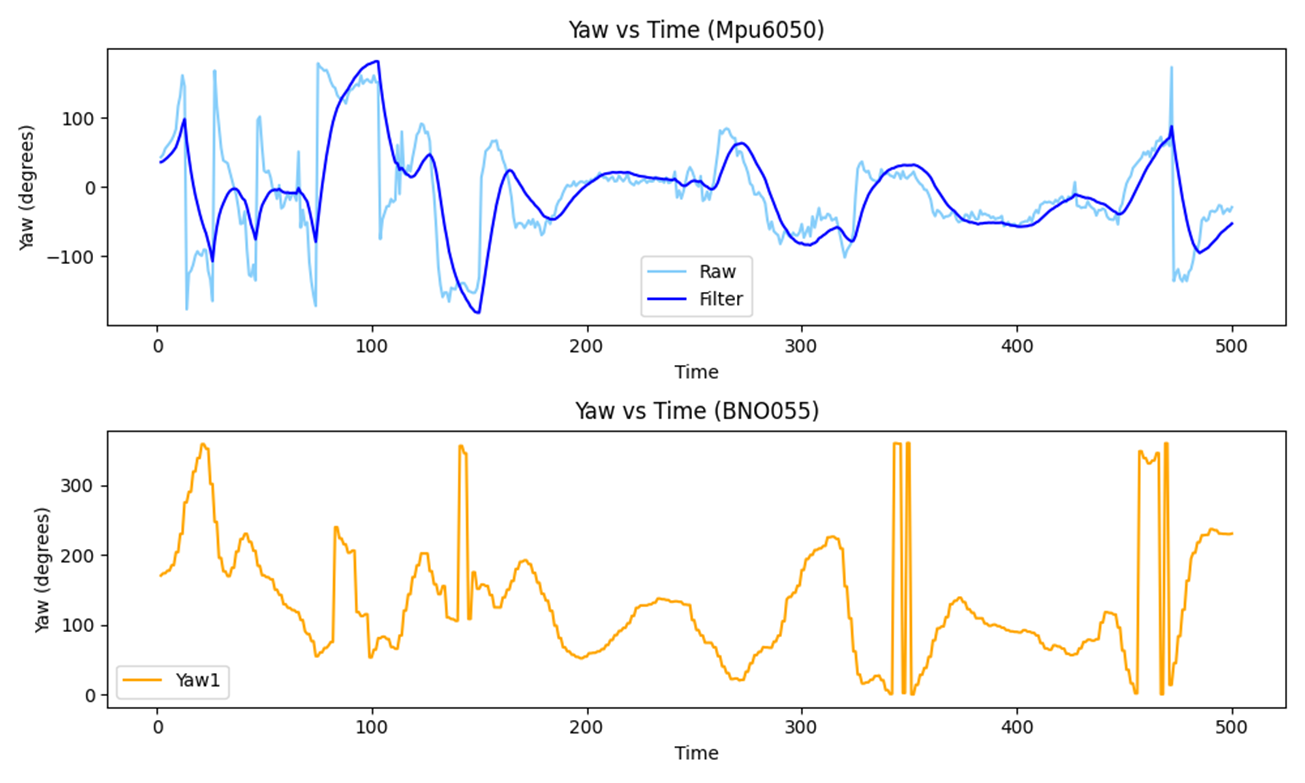
\includegraphics[width=0.8\textwidth]{Imagenes/Metodologia/Angulos_Giro_pitch_Mpu6050_BNO055.png}
    \caption{Ángulos de Giro Pitch obtenidos con \textbf{MPU6050} y \textbf{BNO055}.}
    \label{fig:pitch}
\end{figure}

\begin{figure}[H]
    \centering
    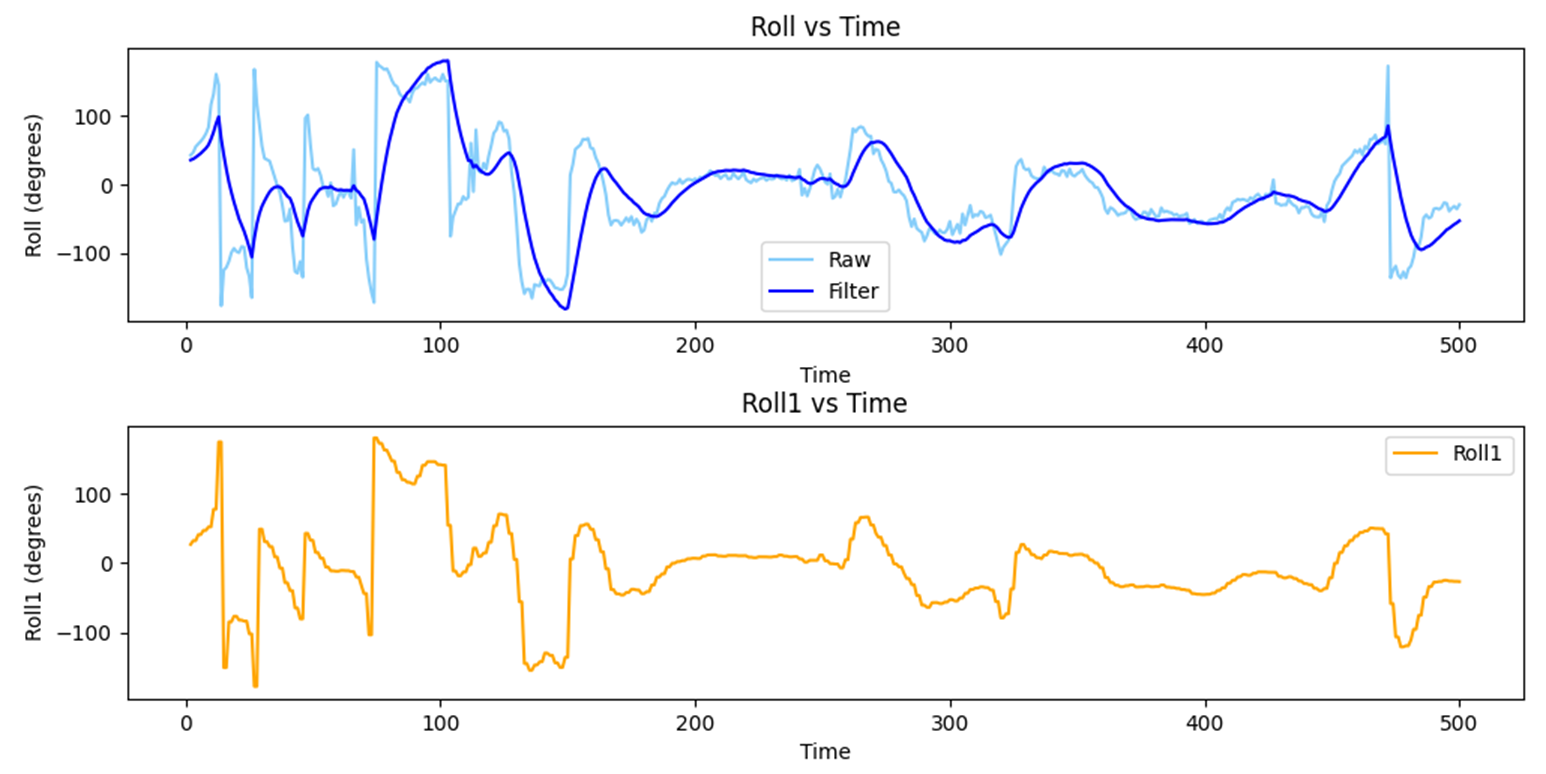
\includegraphics[width=0.8\textwidth]{Imagenes/Metodologia/Angulos_Giro_roll_Mpu6050_BNO055.png}
    \caption{Ángulos de Giro Roll obtenidos con \textbf{MPU6050} y \textbf{BNO055}.}
    \label{fig:roll}
\end{figure}

\begin{figure}[H]
    \centering
    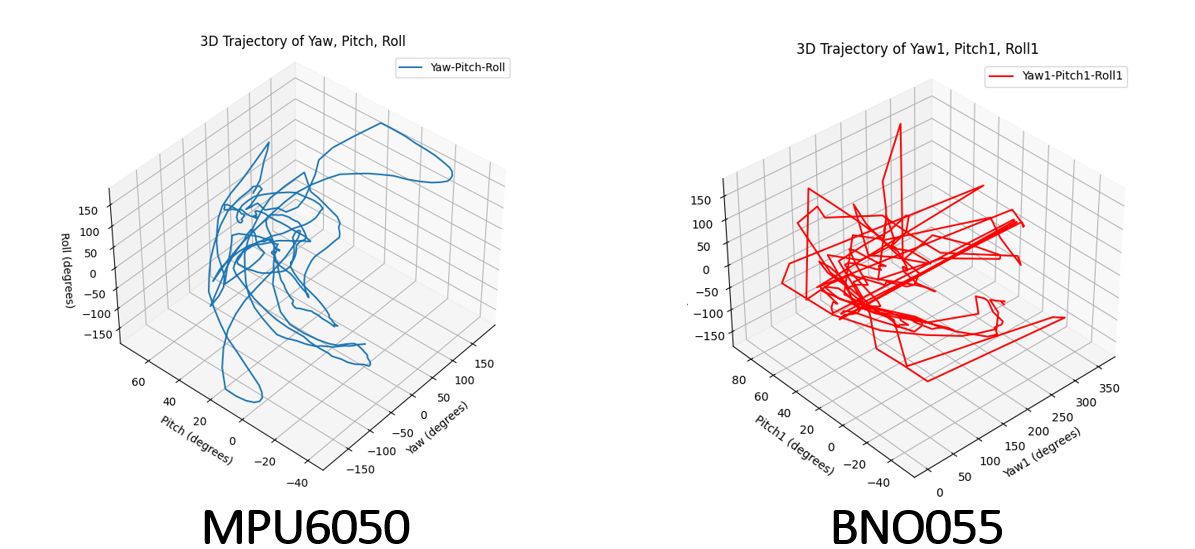
\includegraphics[width=0.8\textwidth]{Imagenes/Metodologia/Angulos_Giro_Mpu6050_BNO055.png}
    \caption{Ángulos de Giro \textbf{MPU6050} y \textbf{BNO055}.}
    \label{fig:3d_trajectory}
\end{figure}

\\ \\
\paragraph{ \large \textbf{Protocolo de Inicialización y Recepción de Datos del BNO055}}

\\ \\
\begin{enumerate}
    \item \textbf{Detección del Sensor}:
    \begin{itemize}
        \item El sensor \textbf{BNO055} se inicializa y se intenta establecer comunicación en la dirección I2C predeterminada. Si no se detecta el sensor, se muestra un mensaje de error en el monitor serie.
    \end{itemize}

    \item \textbf{Calibración del Sensor}:
    \begin{itemize}
        \item Se entra en un bucle de calibración donde se verifica continuamente el estado de calibración del sensor. Durante este proceso, se muestra el estado de calibración en una pantalla OLED.
    \end{itemize}

    \item \textbf{Contador de 5 Segundos}:
    \begin{itemize}
        \item Después de la calibración, se muestra un contador de 5 segundos en la pantalla OLED, permitiendo que el usuario coloque el dispositivo en una posición de referencia estable.
    \end{itemize}

    \item \textbf{Cálculo y Visualización de los Offsets}:
    \begin{itemize}
        \item Se calculan los offsets de los ángulos (roll, pitch y yaw) en la posición de referencia y se muestran en la pantalla OLED.
    \end{itemize}
\end{enumerate}
\\ \\
\paragraph{\large Recepción de Datos del \textbf{BNO055}}
\\ \\
\begin{enumerate}
    \item \textbf{Lectura de Datos de Orientación}:
    \begin{itemize}
        \item Se leen los valores de orientación (yaw, pitch y roll) del sensor y se ajustan estos valores restando los offsets calculados previamente.
    \end{itemize}

    \item \textbf{Lectura de Datos del Acelerómetro}:
    \begin{itemize}
        \item Se leen los valores de aceleración en los ejes X, Y y Z.
    \end{itemize}

    \item \textbf{Lectura de Datos del Magnetómetro}:
    \begin{itemize}
        \item Se leen los valores del campo magnético en los ejes X, Y y Z.
    \end{itemize}

    \item \textbf{Cálculo del Valor de la Brújula}:
    \begin{itemize}
        \item Se calcula el valor del heading utilizando los datos del magnetómetro y luego se aplica un filtro de Media Exponencialmente Ponderada (EMA) para suavizar el valor del heading.
    \end{itemize}
\end{enumerate}



\paragraph{\large  \textbf{Cálculo del Heading}}
\\ \\
El heading (rumbo) se calcula utilizando los componentes X e Y del campo magnético:
\\ \\
\[
\text{heading\_rad} = \text{atan2}(my, mx)
\]

\[
\text{heading\_deg} = \text{heading\_rad} \times \frac{180.0}{\pi}
\]
\\ \\
Si el valor calculado del heading es negativo, se ajusta sumándole 360 grados para obtener un valor positivo:
\\ \\
\[
\text{if} \ (\text{heading\_deg} < 0) \ \text{then} \ \text{heading\_deg} += 360
\]

\paragraph{\large Suavizado del Heading con EMA}
\\ \\
Para reducir la oscilación en los valores de heading, se aplica un filtro de Media Exponencialmente Ponderada (EMA). La fórmula para actualizar el valor suavizado es:
\\ \\
\[
\text{smoothedHeading} = \alpha \times \text{newHeading} + (1 - \alpha) \times \text{oldHeading}
\]

Donde \(\alpha\) es el factor de suavizado. Para manejar la discontinuidad alrededor de 360 grados, se ajusta la diferencia de los valores de heading:

\[
\text{diff} = \text{newHeading} - \text{oldHeading}
\]

\[
\text{if} \ (\text{diff} > 180) \ \text{then} \ \text{oldHeading} += 360
\]

\[
\text{else if} \ (\text{diff} < -180) \ \text{then} \ \text{oldHeading} -= 360
\]

Finalmente, se ajusta el valor suavizado para mantenerse dentro del rango de 0 a 360 grados:
\\ \\
\[
\text{if} \ (\text{smoothedHeading} \geq 360) \ \text{then} \ \text{smoothedHeading} -= 360
\]

\[
\text{else if} \ (\text{smoothedHeading} < 0) \ \text{then} \ \text{smoothedHeading} += 360
\]
\\ 
Este método asegura que los valores de heading se mantengan dentro del rango de 0 a 360 grados y se suavicen adecuadamente, reduciendo las fluctuaciones en la señal.
\\ \\
\subsubsection{Barómetro, Altímetro y Termómetro}
\\ \\
Un barómetro es un instrumento capaz de medir la presión atmosférica, proporcionando datos esenciales para la predicción del tiempo y la altitud. En el contexto de sensores modernos, como el \textbf{BMP280}, estas funcionalidades se amplían significativamente. El BMP280 no solo actúa como un barómetro, sino que también integra un altímetro y un termómetro. Esto permite obtener medidas precisas de presión, altitud y temperatura en un solo dispositivo compacto. La capacidad de medir la presión atmosférica es crucial para determinar la altitud en aplicaciones de navegación y control de un UAV de ala fija, mientras que la medición de la temperatura ayuda a saber la temperatura del controlador de vuelo.\\ \\
\paragraph{\large  \textbf{Inicialización del BMP280}}\\ \\

Al iniciar el sensor BMP280, se configura la presión atmosférica de referencia para \textbf{Bogotá} en \textbf{1028} hPa. Luego, se lee la altura inicial basada en esta referencia. Si la inicialización del sensor falla, se imprime un mensaje de error en el monitor serial. El proceso de inicialización garantiza que las lecturas de altura sean precisas y consistentes con la altitud específica de Bogotá.
\\ \\
\paragraph{\large  \textbf{Aplicación del EMA (Exponential Moving Average)}}\\ \\

Para suavizar las lecturas de presión atmosférica, altura y temperatura interna del dispositivo, se está aplicando un algoritmo de Media Móvil Exponencial (EMA). Este algoritmo es útil para reducir el ruido en los datos y proporcionar valores más estables y representativos. El EMA calcula el promedio ponderado de los datos recientes, donde los datos más recientes tienen un peso mayor en el cálculo del promedio. Esto se realiza para cada una de las mediciones (presión, altura y temperatura) obtenidas del BMP280. \\

La fórmula utilizada para el cálculo del EMA es la siguiente:
\\ \\
\[
\text{EMA} = (\alpha \cdot \text{currentReading}) + ((1 - \alpha) \cdot \text{previousEMA})
\]
\\ \\
Donde:
\begin{itemize}
    \item \text{currentReading} es la lectura actual del sensor.
    \item \text{previousEMA} es el valor del EMA anterior.
    \item $\alpha$ es el factor de suavizado, un valor entre 0 y 1 que determina el peso de la lectura actual en el cálculo del EMA.
\end{itemize}
\\ \\
\paragraph{\large  \textbf{Proceso de Lectura de Datos}}
\\ \\
\begin{enumerate}
    \item \textbf{Presión Atmosférica}: Se obtiene directamente del sensor y se aplica el EMA para suavizar las lecturas.
    \item \textbf{Altura}: Se calcula en función de la presión atmosférica y se ajusta utilizando la altura inicial leída durante la inicialización. También se aplica el EMA para obtener una lectura más estable.
    \item \textbf{Temperatura Interna}: Se mide directamente desde el BMP280 y se procesa mediante el EMA para reducir el ruido en las lecturas.
\end{enumerate}\\ \\



\subsubsection{Sistema de Posicionamiento Global (GPS)}\\ \\


Para asegurar una alta fiabilidad y precisión en la ubicación del UAV, se seleccionó el \textbf{GPS M10Q-5883}. Este dispositivo integra el módulo GNSS SAM-M10Q-00B de u-blox, capaz de recibir simultáneamente señales de cuatro constelaciones \textbf{satelitales: GPS, GLONASS, Galileo y BeiDou}.\cite{GPS} Esta capacidad multiconstelación amplía significativamente la cobertura y mejora la disponibilidad de la señal en condiciones adversas, como en entornos urbanos densos o áreas con obstrucciones. Además, el módulo GNSS SAM-M10Q-00B emplea tecnología avanzada que optimiza la sensibilidad y reduce el tiempo de adquisición de señal, garantizando así una ubicación precisa y dinámica incluso en escenarios complicados. Utilizando el protocolo de comunicaciones UART, este sistema transmite datos de posición de manera precisa y confiable, asegurando que el UAV pueda navegar y operar de forma óptima en diversas condiciones. \\ \\

\paragraph{\large  \textbf{Proceso de Inicialización del GPS}}
Para inicializar el GPS es necesario establecer la comunicación serial con el dispositivo. Esto se logra utilizando el siguiente código, que configura los pines TX2 y RX2 para la comunicación serial: \\ \\
\begin{lstlisting}[language=C++]
const int TX2 = 11;
const int RX2 = 10;
Serial2.begin(9600, SERIAL_8N1, RX2, TX2);
\end{lstlisting}

\\ \\

Una vez que el GPS está conectado y se inicializa la comunicación serial, el dispositivo se encenderá con una luz verde. Es importante situar el GPS en un lugar con cielo abierto, ya que tardará unos minutos en obtener la recepción de las señales de los satélites. Una vez que el módulo recibe la señal de los satélites, comenzará a titilar, indicando que se ha establecido correctamente la comunicación con el satélite. \\

Para contrastar y validar que los valores recibidos por el GPS eran correctos, se utilizó la aplicación GnssLogger de Google (véase la Figura \ref{fig:gpsGnss}). En esta prueba, se compararon los datos obtenidos por el GPS con los proporcionados por la red WLS (Wireless Location Service) y el GPS del celular. La prueba se realizó en la terraza del quinto piso del edificio Mario Laserna. Se encontró que todos los datos de ubicación se encontraban dentro de un radio de aproximadamente 6 metros, lo que confirma la precisión de los datos recibidos. \\ 

\begin{figure}[H]
    \centering
    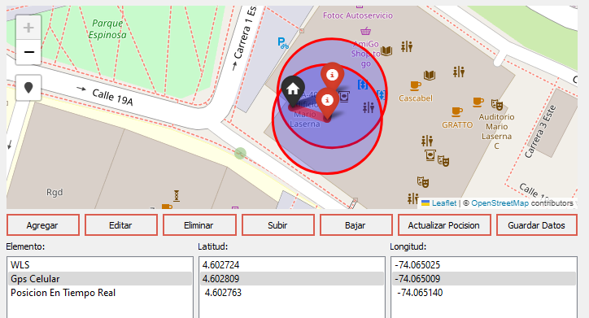
\includegraphics[width=10 cm]{Imagenes/Firmware/GPS.png}
    \caption{Validación de la precisión del GPS utilizando GnssLogger.}
    \label{fig:gpsGnss}
\end{figure}



%\subsection{Pantalla Oled 1,3}

\\ \\
\subsection{Recopilación y Almacenamiento de Datos}
\\ \\
En el ámbito de las aeronaves, la recopilación y el almacenamiento de datos juegan un papel crucial. Este dispositivo es esencial, ya que permite registrar la información histórica del vuelo, proporcionando un registro detallado de todos los eventos y parámetros operativos. Actúa como una "caja negra" que almacena datos vitales que pueden ser utilizados para análisis post-vuelo, mantenimiento preventivo, y en el desafortunado caso de una eventualidad, para la investigación de incidentes. La capacidad de recopilar y almacenar datos de manera confiable asegura que toda la información relevante del vuelo esté disponible para su revisión.
\subsubsection{SD TF}

El módulo lector de microSD, también conocido como SD (Secure Digital), es un componente esencial en el dispositivo. Este módulo permite guardar la información y los datos generados por los sensores y los cálculos realizados por la \textbf{ESP32-S3}. La microSD funciona mediante un sistema de archivos que permite almacenar y recuperar datos de forma eficiente y confiable. Al inicializar la comunicación con el módulo a través de la \textbf{ESP32-S3}, se pueden escribir y leer datos en la tarjeta microSD. La información recopilada se almacenará en formato CSV (Comma-Separated Values), lo que facilita la organización y el análisis posterior de los datos.
\begin{figure}[H]
    \centering
    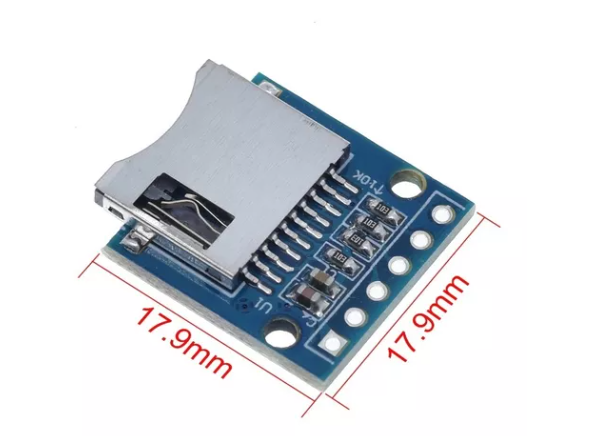
\includegraphics[width=2 in]{Imagenes/Metodologia/SD.png}
    \caption{Lector de tarjetas MicroSD}
    \label{fig:microSD}
\end{figure}
\textbf{Especificaciones Técnicas}
\begin{itemize}
    \item Modelo: Módulo lector SD TF
    \item Interfaz: SPI
    \item Voltaje de operación: 3.3V - 5V
    \item  Compatibilidad: Tarjetas microSD
\end{itemize} \\ \\
\subsubsection{Conexión y Configuración} \\\\

El módulo lector SD se comunica con el ESP32-S3 a través del protocolo SPI. A continuación, se detallan las conexiones entre el módulo lector SD y el ESP32-S3: \\ \\

\begin{itemize}
    \item MISO (Master In Slave Out): Conectado al pin MISO del ESP32-S3   \textbf{GPIO 37}
    \item MOSI (Master Out Slave In): Conectado al pin MOSI del ESP32-S3  \textbf{GPIO 35}
    \item SCK (Serial Clock): Conectado al pin SCK del ESP32-S3        \textbf{GPIO 36}
    \item CS (Chip Select): Conectado a un pin GPIO del ESP32-S3       \textbf{GPIO 38}
\end{itemize} \\ \\




\subsection{Telecomunicaciones}

En el apartado de telecomunicaciones es importante resaltar la presencia de dos componentes principales que son cruciales para el control y monitoreo del UAV. \\ 

El primer componente es el módulo de radiofrecuencia, el cual se encarga de recibir la información del operador de vuelo. Este módulo permite que la aeronave responda a los comandos enviados por el operador, facilitando el control y la maniobrabilidad del UAV. La comunicación por radiofrecuencia es esencial para asegurar que los comandos se transmitan de manera eficiente y sin retrasos, permitiendo una respuesta inmediata del UAV a las instrucciones del operador.\\ 

El segundo componente es el módulo de telemetría, que tiene la capacidad de recibir información del UAV en tiempo real. Este módulo proporciona datos vitales sobre el estado y la posición de la aeronave, incluyendo parámetros como la altitud, velocidad, orientación y otros datos críticos de vuelo. La telemetría en tiempo real es fundamental para el monitoreo continuo del UAV.\\ 
\subsubsection{Módulo de radiofrecuencia Fly-Sky FS-IA6B}

En el apartado de radiofrecuencia, se utilizo el transmisor y receptor FS-i6 de la empresa FlySky el cual es un controlador de radio digital de 6 canales diseñado para ofrecer un control preciso y fiable para diversas aplicaciones de modelismo, como drones, aviones, helicópteros y coches RC. Este transmisor utiliza la tecnología AFHDS 2A (Automatic Frequency Hopping Digital System) para asegurar una comunicación sin interferencias y una alta inmunidad al ruido. \cite{flysky}

\textbf{Características Principales:}
\begin{itemize}
    \item \textbf{Frecuencia:} 2.4 GHz AFHDS 2A.
    \item \textbf{Canales:} 6 canales programables.
    \item \textbf{Pantalla LCD:} Proporciona una interfaz gráfica para la configuración y el monitoreo en tiempo real.\cite{19}
    \item \textbf{Rango de Operación:} Hasta 1 km en condiciones óptimas.\cite{19}
    \item \textbf{Compatibilidad:} Compatible con diversos receptores FlySky que soportan AFHDS 2A.\cite{flysky}
    \item \textbf{Funciones:} Incluye funciones avanzadas como mezcla de canales, configuración de servos, límite de puntos finales, y modos de vuelo.   \cite{flysky}
\end{itemize}

Para interconectar este sistema de radio control con el controlador de vuelo, se procedió a realizar un análisis de cómo sería la comunicación del receptor con el dispositivo (véase \ref{fig:radio_arqui}). Se descubrió que cada uno de los 6 canales del dispositivo envía una señal \textbf{PWM}, por lo que, si se procesa esta información con la \textbf{ESP32-S3} y se decodifica esta señal, es posible transcribir este ancho de pulso en valores para que la \textbf{PCA9685} pueda mover los servos al valor deseado.


\begin{figure}[H]
    \centering
    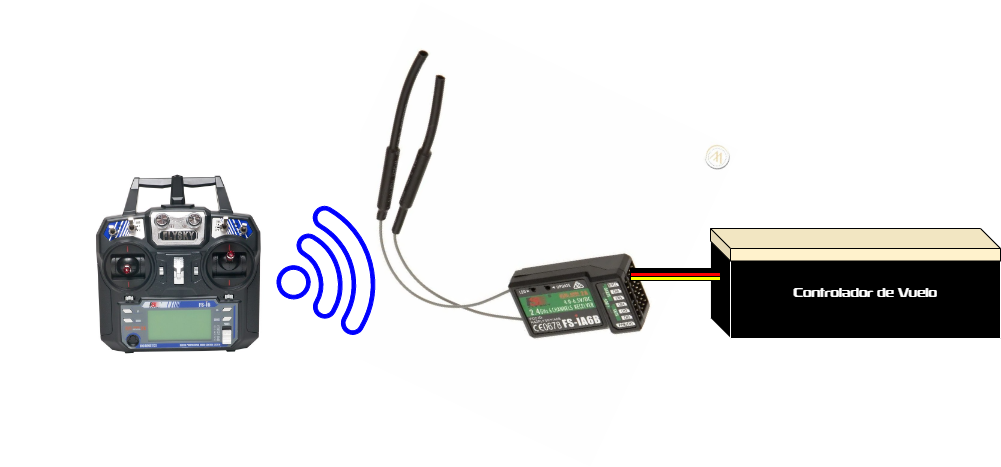
\includegraphics[width=6 in]{Imagenes/Metodologia/Radio Control.drawio.png}
    \caption{Conexión del Radio Control con el Controlador de Vuelo}
    \label{fig:radio_arqui}
\end{figure}

Este sistema se realizó de esta forma ya que es posible decodificar la información del transmisor  \textbf{Fly-Sky FS-IA6B} y poder efectuar una respuesta en los actuadores de la aeronave. Es importante destacar el hecho de al estar leyendo la información y posteriormente  enviando esta información a los \textbf{servos} se genera un pequeño \textbf{delay} que debe tenerse en cuenta al momento de operar la aeronave.

\vspace{5 px}
\paragraph{\textbf{Proceso de Decodificación}}
\vspace{5 px}
Para decodificar las señales PWM, se utiliza la función \texttt{pulseIn} del microcontrolador, que mide la duración del pulso en microsegundos. Esta duración se mapea a un rango de valores especificado mediante la función \texttt{map}.
\vspace{5 px}
\paragraph{\textbf{Medición del Pulso}}
\vspace{5 px}
La función \texttt{pulseIn} mide el tiempo durante el cual la señal es alta (nivel lógico alto). Esta duración, \( t \), se expresa en microsegundos (\(\mu\)s). El rango típico de estas duraciones para las señales PWM del receptor FLYSKY-I6B es:

\begin{equation*}
t \in [1007 \, \mu s, 1999 \, \mu s]
\end{equation*}
\vspace{5 px}
\paragraph{\textbf{Mapeo de la Señal}}
\vspace{5 px}
Para convertir la duración del pulso a un valor utilizable, se utiliza la función \texttt{map}. La función mapea el rango de entrada \([1007, 1999]\) a un rango de salida especificado por los parámetros \texttt{minLimit} y \texttt{maxLimit}. Estos parámetros descritos anteriormente hacen referencia al valor máximo y mínimo al que pueden llegar cada uno de los servomotores de la aeronave, típicamente este valor es \textbf{-30°} y \textbf{30°} con respecto al valor de referencia inicial del servo, el cual generalmente es de \textbf{90°}. A continuación se muestra la ecuación de mapeo:


\begin{equation*}
y = \frac{(\texttt{maxLimit} - \texttt{minLimit})}{(1999 - 1007)} \cdot (t - 1007) + \texttt{minLimit}
\end{equation*}
\vspace{5 px}
\paragraph{\textbf{Condiciones de Valor por Defecto}}
\vspace{5 px}
Si la duración del pulso \( t \) es menor que 100 $\mu$s, se asume que la señal es inválida, y se devuelve un valor por defecto, \texttt{defaultValue}.
\vspace{5 px}
\paragraph{\textbf{Lectura de Interruptores}}
\vspace{5 px}
Para leer el estado de un interruptor, se convierte la señal PWM del canal correspondiente a un valor booleano (verdadero o falso). Este proceso implica mapear la señal a un rango de 0 a 100 y determinar si el valor resultante es mayor que 50. La ecuación de mapeo en este caso es:

\begin{equation}
z = \frac{(100 - 0)}{(1999 - 1007)} \cdot (t - 1007) + 0
\end{equation}

El resultado se evalúa para determinar el estado del interruptor:

\begin{equation}
\text{estado} = 
\begin{cases} 
\text{verdadero} & \text{si } z > 50 \\
\text{falso} & \text{si } z \leq 50 
\end{cases}
\end{equation}

A continuación se muestra un esquema (\ref{fig:decodificador_transmisor}) del transmisor FLYSKY-I6B y los valores decodificados de cada uno de los seis canales. Nótese que el \textbf{canal 1} hace referencia al movimiento de \textbf{roll}, el \textbf{canal 2} a \textbf{pitch} y el \textbf{canal 4} a \textbf{yaw} de la aeronave, controlando cada uno un servomotor que representa un movimiento particular de esta. El \textbf{canal 3} se encarga de controlar el suministro de combustible al motor. Finalmente, los canales \textbf{5 y 6} son interruptores.


\begin{figure}[H]
    \centering
    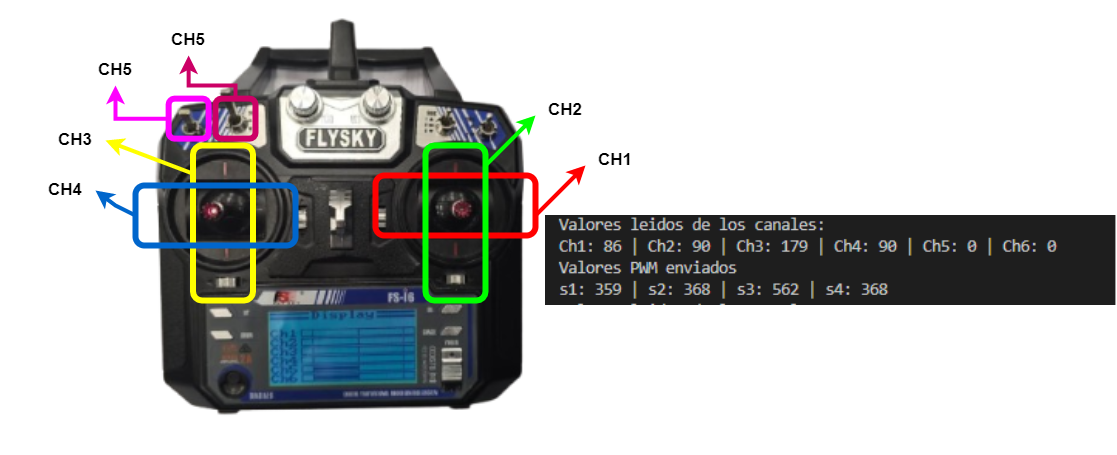
\includegraphics[width=6 in]{Imagenes/Metodologia/Diagrama Receptor.png}
    \caption{Diagrama Transmisor y decodificado de Señales PWM}
    \label{fig:decodificador_transmisor}
\end{figure}



\subsection{Telemetría}





\subsubsection{Módulo nRF24L01}\\ \\

El módulo nRF24L01 es un transceptor inalámbrico que opera en la banda de 2.4 GHz, una frecuencia comúnmente utilizada para comunicaciones de corto alcance debido a su equilibrio entre velocidad de transmisión y penetración de obstáculos. Este módulo es conocido por su bajo consumo de energía y su capacidad para manejar comunicaciones de hasta 2 Mbps.\\ 

Una de las limitaciones del nRF24L01 es su capacidad para manejar paquetes de datos de hasta 32 bits. Esto significa que los datos transmitidos deben ser empaquetados para evitar la pérdida o corrupción de la información.

\subsubsection{Estación en Tierra }\\ \\

La estación en tierra es un circuito igual que el controlador de vuelo que permite la transmisión y recepción de datos entre la aeronave y el equipo en tierra. Esta comunicación se realiza utilizando el módulo nRF24L01, previamente descrito. \\


La estación en tierra recibe los datos transmitidos por el controlador de vuelo, una vez interpretados, envía un mensaje de confirmación de recepción al controlador de vuelo. Este proceso bidireccional asegura que los datos de telemetría sean correctamente. \\

El funcionamiento de la comunicación se puede observar en la figura \ref{fig:estacion en tierra}, donde se muestra el flujo de mensajes entre la estación en tierra y el controlador de vuelo: \\ \\ 

\begin{itemize}
    \item \textbf{Transmisión:} El controlador de vuelo envía datos a la estación en tierra codificados.
    \item \textbf{Recepción:} La estación en tierra recibe los datos y los decodifica.
    \item \textbf{Mensaje de Verificación:} La estación en tierra envía un mensaje de verificación de recepción.
    \item \textbf{Confirmación:} El controlador de vuelo recibe la confirmación de que los datos fueron recibidos.
\end{itemize} \\ \\ 

Este ciclo continuo de transmisión y verificación es esencial para mantener la integridad de los datos y garantizar que cualquier ajuste necesario durante el vuelo se base en información precisa y actualizada.\\ \\ 
\begin{figure}[H]
    \centering
    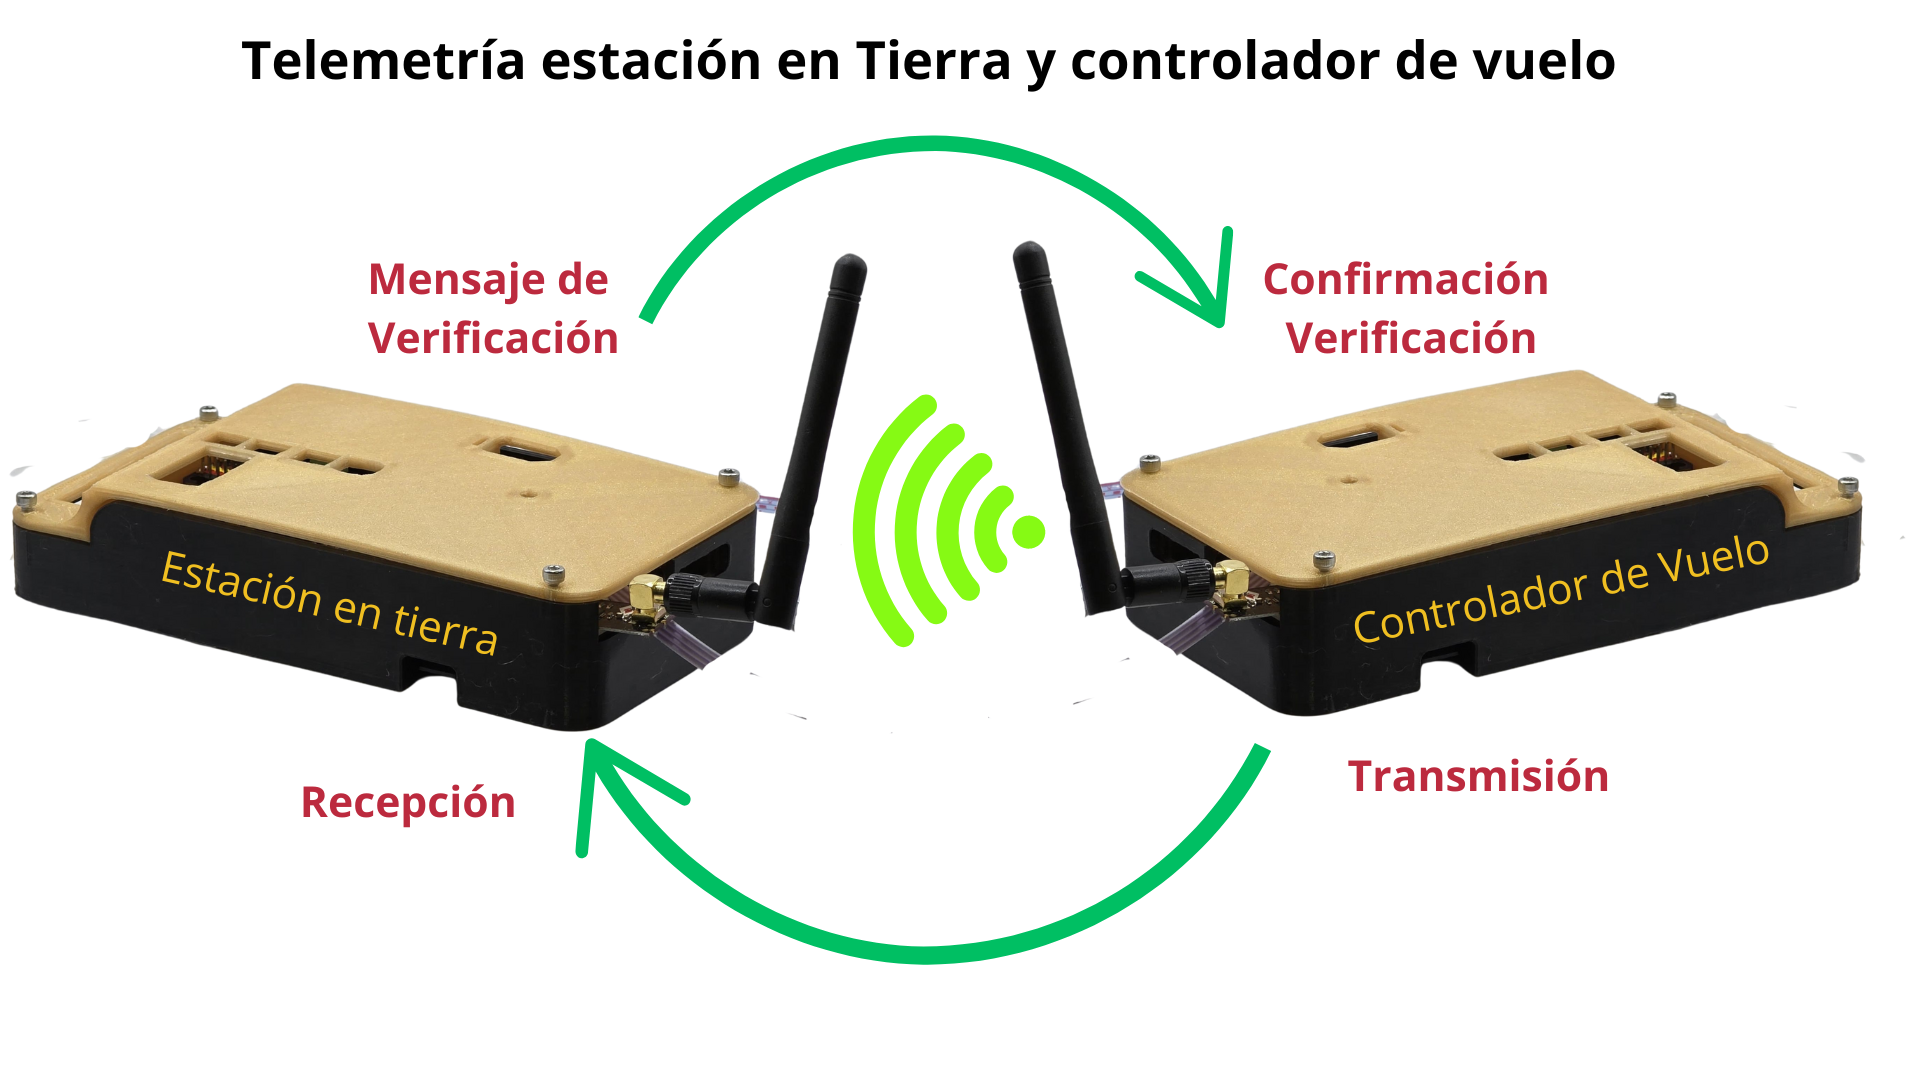
\includegraphics[width=\textwidth]{Imagenes/Metodologia/estacion en tierra.png}
    \caption{Conexión del Controlador de Vuelo y la estación en Tierra}
    \label{fig:estacion en tierra}
\end{figure} \\ \\ 



\subsubsection{Arquitectura General del Firmware Controlador de Vuelo y la Estación de Control en Tierra} \\  \\ 


La figura \ref{fig:diag-codigo } representa la arquitectura general del controlador de vuelo y la estación de control en tierra, detallando los protocolos de inicialización y las principales tareas realizadas por cada sistema. A continuación se presenta una explicación general de cada sección:\\ \\ 

\subsection{Controlador de Vuelo}\\  \\ 

\begin{itemize}
    \item \textbf{Protocolo de Inicialización}
    \begin{itemize}
        \item \textbf{Escaneo e Inicialización de Dispositivos I2C}: El sistema escanea e inicializa todos los dispositivos I2C conectados al controlador de vuelo.
        \item \textbf{Inicialización del Protocolo SPI y Creación del Archivo de Datos}: Se inicializa el protocolo SPI y se crea un archivo de datos para almacenar los datos de vuelo.
    \end{itemize}
    \\ \\ 
    \item \textbf{Bucle Principal (Mientras Está Encendido)}
    \begin{itemize}
        \item \textbf{Lectura de Sensores y GPS, Actualización de Variables Globales y Pantalla OLED}: El controlador de vuelo lee datos de varios sensores y del módulo GPS, actualiza las variables globales y la pantalla OLED.
        \item \textbf{Lectura de Canales del Receptor}: El sistema lee las entradas de los canales del receptor, que contienen los comandos de control de la estación de control en tierra o del operador.
        \item \textbf{Escritura de Datos en la MicroSD}: Los datos de vuelo se escriben en una tarjeta MicroSD para su registro y análisis posterior.
        \item \textbf{Envío de Datos (Telemetría)}: Los datos de telemetría comprimidos en 32 bits se envían a la estación de control en tierra.
    \end{itemize}
    \\ \\ 
    \item \textbf{Tarea: Escritura y Movimiento de Actuadores}
    \begin{itemize}
        \item \textbf{Determinación del Modo de Operación Basado en Comandos y Datos de Vuelo}: El controlador de vuelo determina el modo de operación del UAV basado en los comandos de entrada y los datos de vuelo actuales.
        \item \textbf{Mover Actuadores}: El sistema envía comandos a los actuadores para controlar los movimientos del UAV.
    \end{itemize}
\end{itemize}
\\  \\ 
\subsection{Estación de Control en Tierra}

\begin{itemize}
    \item \textbf{Protocolo de Inicialización}
    \begin{itemize}
        \item \textbf{Escaneo e Inicialización de Dispositivos I2C}: Similar al controlador de vuelo, la estación de control en tierra escanea e inicializa todos los dispositivos I2C conectados.
        \item \textbf{Inicialización del Protocolo SPI y Creación del Archivo de Datos}: Se inicializa el protocolo SPI y se crea un archivo de datos para almacenar los datos recibidos.
    \end{itemize}
    \\  \\ 
    \item \textbf{Bucle Principal (Mientras Está Encendido)}
    \begin{itemize}
        \item \textbf{Lectura de Información de Radio}: La estación de control en tierra lee los datos recibidos vía radio desde el controlador de vuelo.
        \item \textbf{Decodificación de la Información}: Los datos recibidos se decodifican para su procesamiento.
        \item \textbf{Escritura de Datos en Serial}: Los datos decodificados se escriben en la interfaz serial para su monitoreo en tiempo real o procesamiento adicional.
        \item \textbf{Escritura de Datos en la MicroSD}: Los datos recibidos y decodificados también se registran en una tarjeta MicroSD para su análisis posterior.
    \end{itemize}
\end{itemize}
\begin{figure}[H]
    \centering
    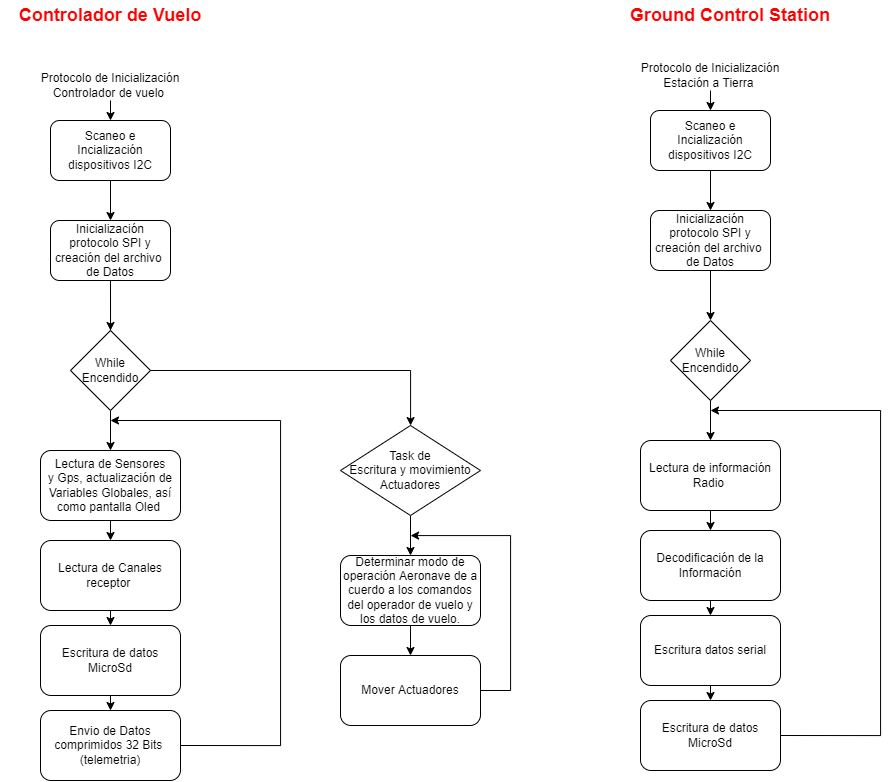
\includegraphics[width=\textwidth]{Imagenes/Interfaz/diagrama general de codigo.png}
    \caption{Diagrama general de funcionamiento Controlador y estación a Tierra }
    \label{fig:diag-codigo }
\end{figure} \\ \\




\subsection{Actuadores} \\ \\


En términos de actuadores, se trabajará con servomotores, ya que son los encargados de mover las superficies de control de la aeronave, incluyendo los alerones, timón de cola, elevadores y el sistema de propulsión eléctrico o de gasolina. \\ 

Para manejar estos distintos actuadores, se seleccionó el módulo \textbf{PCA9685} debido a su capacidad de controlar hasta 16 servomotores o actuadores simultáneamente mediante señales \textbf{PWM}. Este módulo ofrece una gestión precisa y eficiente de los componentes mecánicos de la aeronave. La elección del \textbf{PCA9685} permite una optimización del diseño y la funcionalidad del UAV, facilitando la implementación de sistemas de control complejos con una sola placa. Esto reduce la necesidad de múltiples controladores y simplifica la arquitectura del sistema. \\ \\

\subsubsection{Funcionamiento}

A la hora de leer los valores del radiotransmisor FlySky, es importante recordar que estamos mapeando la señal que devuelve en un valor angular, lo que permite al controlador determinar el ángulo al que debe fijar el servomotor. Para mover los servomotores, se debe convertir ese ángulo en un ancho de pulso PWM válido. El proceso se describe en el siguiente código: \\ 


\begin{lstlisting}[language=C++, caption=Conversión de ángulo a ancho de pulso PWM]
#define MIN_PULSE_WIDTH 600
#define MAX_PULSE_WIDTH 2600

int ReguladorServos::pulseWidth(int angle)
{
    // Función que convierte un ángulo entre 0 y 180 a un ancho de pulso (dato que leen los servos)
    int pulse_wide, analog_value;
    pulse_wide = map(angle, 0, 180, MIN_PULSE_WIDTH, MAX_PULSE_WIDTH);
    analog_value = int(float(pulse_wide) / 1000000 * FREQUENCY * 4096);
    return analog_value;
}
\end{lstlisting}

Definición de los límites del ancho de pulso:\\ 

\begin{itemize}
\item \texttt{#define MIN\_PULSE\_WIDTH 600}: Define el ancho de pulso mínimo en microsegundos.
\item \texttt{#define MAX\_PULSE\_WIDTH 2600}: Define el ancho de pulso máximo en microsegundos.
\end{itemize}

Función de conversión de ángulo a ancho de pulso:\\ 

Definición de los límites del ancho de pulso:\\

\begin{itemize}
\item \texttt{\#define MIN\_PULSE\_WIDTH 600}: Define el ancho de pulso mínimo en microsegundos.
\item \texttt{\#define MAX\_PULSE\_WIDTH 2600}: Define el ancho de pulso máximo en microsegundos.
\end{itemize}

Función de conversión de ángulo a ancho de pulso:\\

\begin{itemize}
\item La función \texttt{pulseWidth(int angle)} toma un ángulo como parámetro, que debe estar en el rango de 0 a 180 grados.
\item Se utiliza la función \texttt{map()} para convertir el ángulo en un ancho de pulso proporcional entre los valores mínimos y máximos definidos.
\item La conversión del ancho de pulso a un valor analógico adecuado para el servomotor se realiza mediante el cálculo: \texttt{analog\_value = int(float(pulse\_wide) / 1000000 * FREQUENCY * 4096);}.
\item La función devuelve este valor analógico, que representa el ancho de pulso PWM requerido para mover el servomotor al ángulo deseado.
\end{itemize}
\\ \\
Este proceso asegura que los ángulos mapeados desde la señal del radiotransmisor se conviertan correctamente en pulsos PWM que los servomotores puedan interpretar. \\ \\




\subsubsection{Movimiento Superficies de Control} \\ \\

Una vez interpretadas las señales del radiocontrol por el receptor y decodificados los ángulos deseados por el operador de vuelo, se asignan valores de movimiento a los servomotores correspondientes a las superficies de control de la aeronave. El canal 1 del receptor controla los alerones, ilustrados en la figura \ref{fig:mov-Superficies } en color morado, que manejan el roll (balanceo lateral). El canal 2 controla los elevadores , en color negro, encargados del pitch (inclinación longitudinal). El canal 3 está conectado al acelerador, regulando la potencia del motor, mientras que el canal 4 controla el timón de cola para el yaw (giro horizontal), en color verde.
\\ \\
\begin{figure}[H]
    \centering
    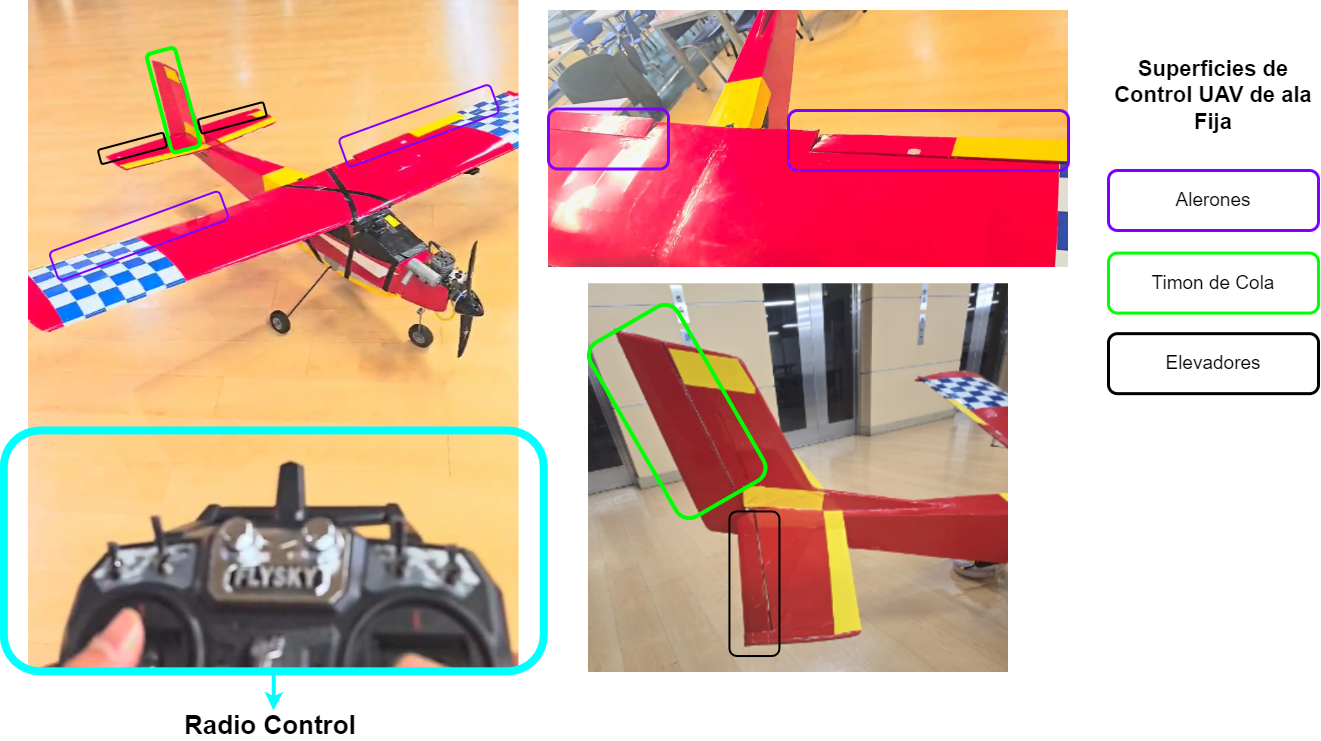
\includegraphics[width=\textwidth]{Imagenes/Firmware/Superficies de Control.png}
    \caption{Movimiento general Superficies de Control }
    \label{fig:mov-Superficies }
\end{figure} \\ \\

\\ \\
\subsection{Control} \\ \\

Para el control básico de la aeronave se estableció el siguiente modelo, en el que el operador de vuelo proporciona una señal de referencia para orientar la aeronave. Esta señal de referencia es un valor angular que indica la posición deseada. Este diagrama de PID está simplificado, ya que cada superficie de control tiene su propio PID para alcanzar la señal de referencia (véase imagen \ref{fig:pid1 }). Seguidamente, el procesador interpreta la señal de referencia que el operador de vuelo desea establecer y mueve la superficie de control correspondiente a cada señal dada por el operador. Este sistema tiene en cuenta las perturbaciones ambientales y se retroalimenta con los valores obtenidos por las unidades de movimiento inerciales (IMUs).


\begin{figure}[H]
    \centering
    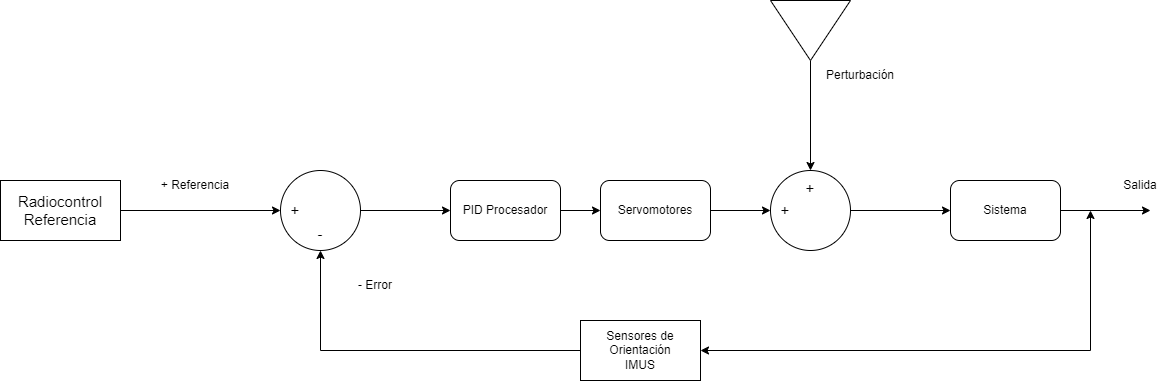
\includegraphics[width=\textwidth]{Imagenes/Firmware/PID basico.png}
    \caption{PID básico Aeronave }
    \label{fig:pid1 }
\end{figure} \\ \\

\subsubsection{Modos de Operación} \\ \\
\begin{itemize}
    \item \textbf{Modo de Vuelo de Autoestabilización:} Este es el modo de operación por defecto. En este modo, si el operador de vuelo no proporciona ninguna señal de referencia, por ejemplo, si el valor de referencia del roll es 0, el UAV de ala fija moverá los alerones para autoestabilizarse y alcanzar este valor de referencia. Este mismo principio se aplica a los ángulos de yaw y pitch, asegurando que la aeronave mantenga su orientación estable.
\\ \\
    \item \textbf{Modo de Operación Fly-by-Wire:} En este modo, el operador de vuelo establece un ángulo de referencia específico para la orientación de la aeronave. Este modo de operación se activa al encender el switch del canal 5. En este modo, el comportamiento del transmisor del radiocontrol es diferente: en lugar de enviar una señal para que un servomotor gire a un ángulo deseado, el operador envía un ángulo de referencia al que desea que esté orientada la aeronave. Los valores de los ángulos están limitados a: \\ \\

\textbf{Roll:} -25° a 25°, puesto que es el ángulo de banqueo máximo permitido para un vehículo aéreo no tripulado. \\ \\
\textbf{Pitch:}-20° a 20°, puesto que es el ángulo de elevación en el que se evita la perdida de sustentación "stall".
\end{itemize}




\subsection{Indicadores Adicionales}
\subsubsection{Dispositivo de visualización}
El sistema de control del UAV incluye un dispositivo de visualización que muestra en tiempo real indicadores cruciales como brújula, temperatura, pitch, roll, altitud, yaw, latitud y longitud. Esto permite al operador verificar el funcionamiento adecuado del UAV durante las pruebas de vuelo, asegurando que los parámetros críticos se mantengan dentro de los límites operativos. El dispositivo facilita el monitoreo continuo, la detección rápida de problemas y la validación de que todos los sistemas responden correctamente.
\begin{figure}[H]
    \centering
    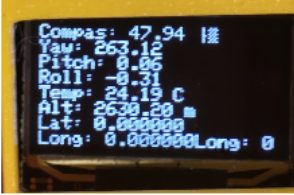
\includegraphics[width=\textwidth]{Imagenes/Firmware/Pantalla oled.png}
    \caption{PID básico Aeronave }
    \label{fig:mov-Superficies }
\end{figure} \\ \\


\subsubsection{Buzzer}

Un \textbf{Buzzer} o \textbf{zumbador} es un componente que se utiliza para emitir señales acústicas. En este caso, se utiliza para proporcionar alertas auditivas en diferentes situaciones. Como lo son la emisión de sonido para informar que el dispositivo se ha inicializado o que se ha conectado el GPS u otros módulos, también puede proporcionar alertas en caso tal de que la batería se este descargando.
\vspace{5 px}
El \textbf{Buzzer} se conecta al \textbf{ESP32-S3} a través de Un pin \textbf{GPIO}, particularmente al \textbf{GPIO-46}  configurado como salida digital. Cuando el microcontrolador envía una señal de alto nivel, el \textbf{Buzzer} emite un sonido en particular alertando al usuario del estado general del sistema.
\vspace{5 px}


\end{comment}



\clearpage
\section{Interfaz}

La interfaz de usuario desarrollada para el UAV de ala fija incluye varios componentes que permiten una visualización integral de los parámetros de vuelo y el estado de la aeronave en tiempo real. Los parámetros considerados más cruciales se han incorporado en diferentes secciones de la interfaz, facilitando el monitoreo y el control efectivo del UAV. A continuación se describen estos componentes:

\subsection{Mapa de Posición en Tiempo Real}

En la figura \ref{fig:mapa Interfaz } se puede observar un apartado en el que se observa la posición del UAV en tiempo real utilizando un mapa interactivo. La posición actual se muestra con coordenadas de latitud y longitud, permitiendo un seguimiento preciso del UAV durante su vuelo.

\begin{figure}[H]
    \centering
    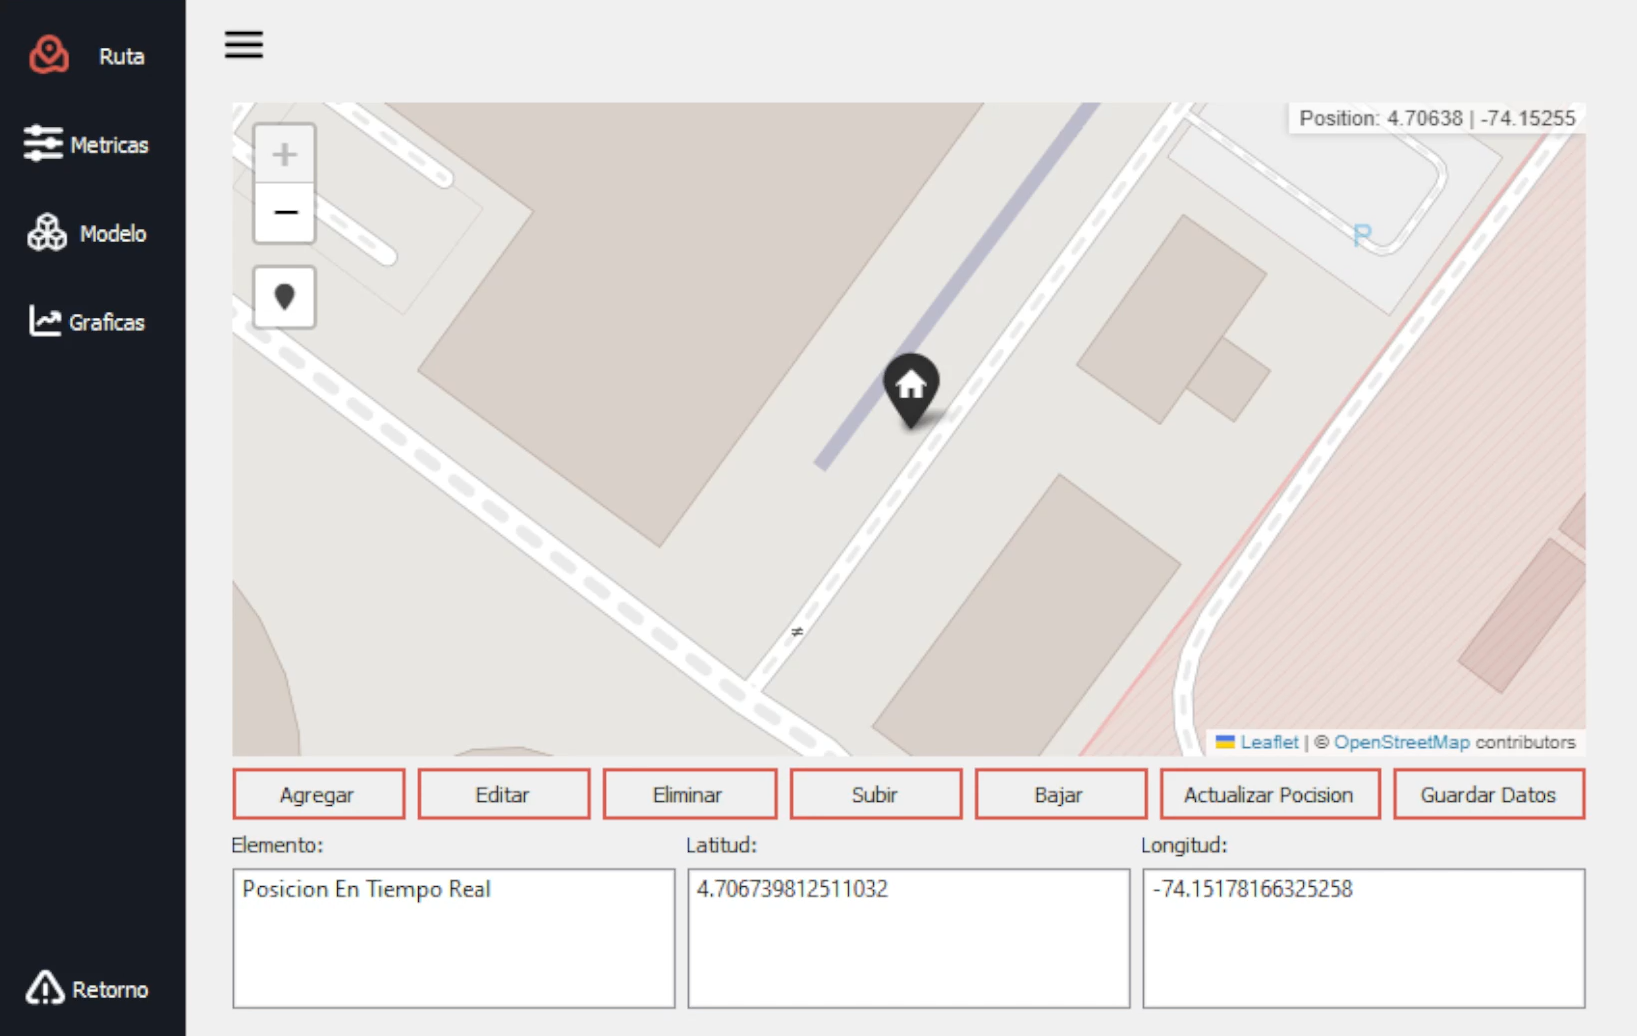
\includegraphics[width=6 in]{Imagenes/Interfaz/mapa_interfaz.png}
    \caption{Mapa de Visualización UAV}
    \label{fig:mapa Interfaz }
\end{figure}

\subsection{Indicadores de Vuelo:}

Las indicadores de vuelo se presentan mediante instrumentos de control similares a los que se encuentran en una aeronave real (véase \ref{fig:metricas interfaz }). Estos instrumentos incluyen:
\begin{itemize}
    \item \textbf{Horizonte Artificial:} Indica la actitud del avión en términos de yaw, pitch y roll.
\item \textbf{Altímetro:} Mide la altitud del UAV con referencia a la altitud inicial del dispositivo.
\item \textbf{Barómetro:}Indica la presión atmosférica.
\item \textbf{Airspeed: }Mide la velocidad del aire.
\item \textbf{Manifold Pressure:} Muestra la presión del colector, relevante para el rendimiento del motor.
\end{itemize}

\begin{figure}[H]
    \centering
    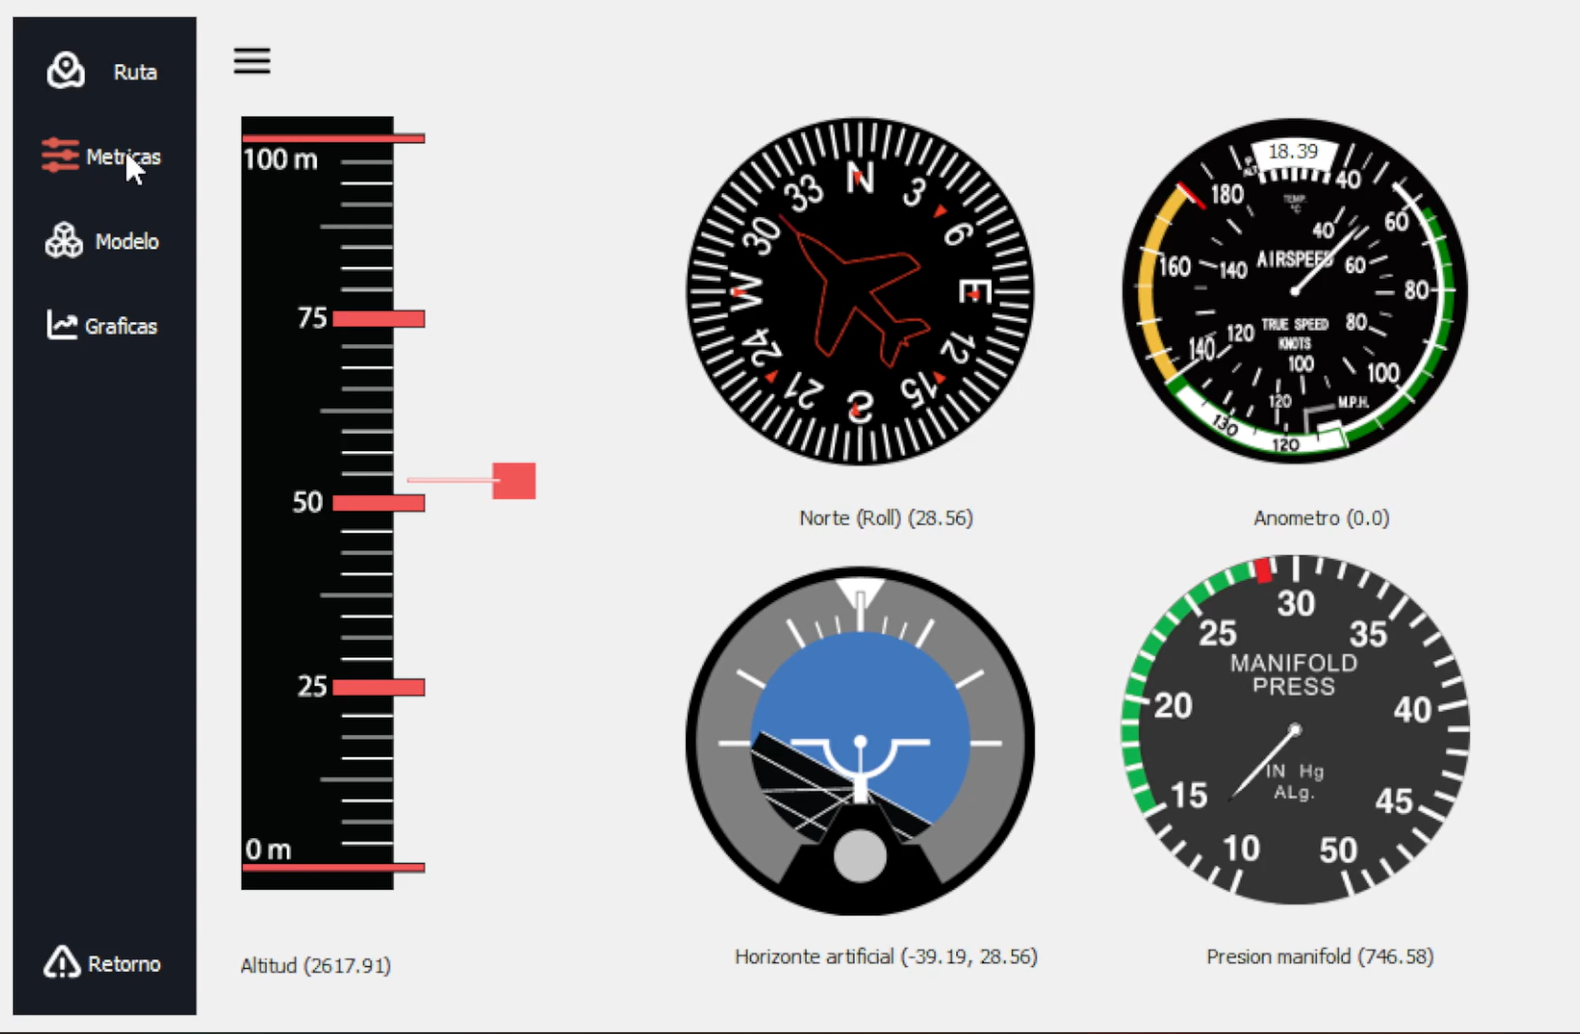
\includegraphics[width=6 in]{Imagenes/Interfaz/metricas.png}
    \caption{indicadores de vuelo para un UAV}
    \label{fig:metricas interfaz }
\end{figure}

\subsection{Modelo 3D del UAV:}

Se incluye un modelo tridimensional del UAV que representa su orientación en el espacio \ref{fig:modelo 3d inerfaz }.  Proporcionando una visualización clara de la dirección hacia donde está apuntando el UAV, facilitando la comprensión de su comportamiento dinámico.
\begin{figure}[H]
    \centering
    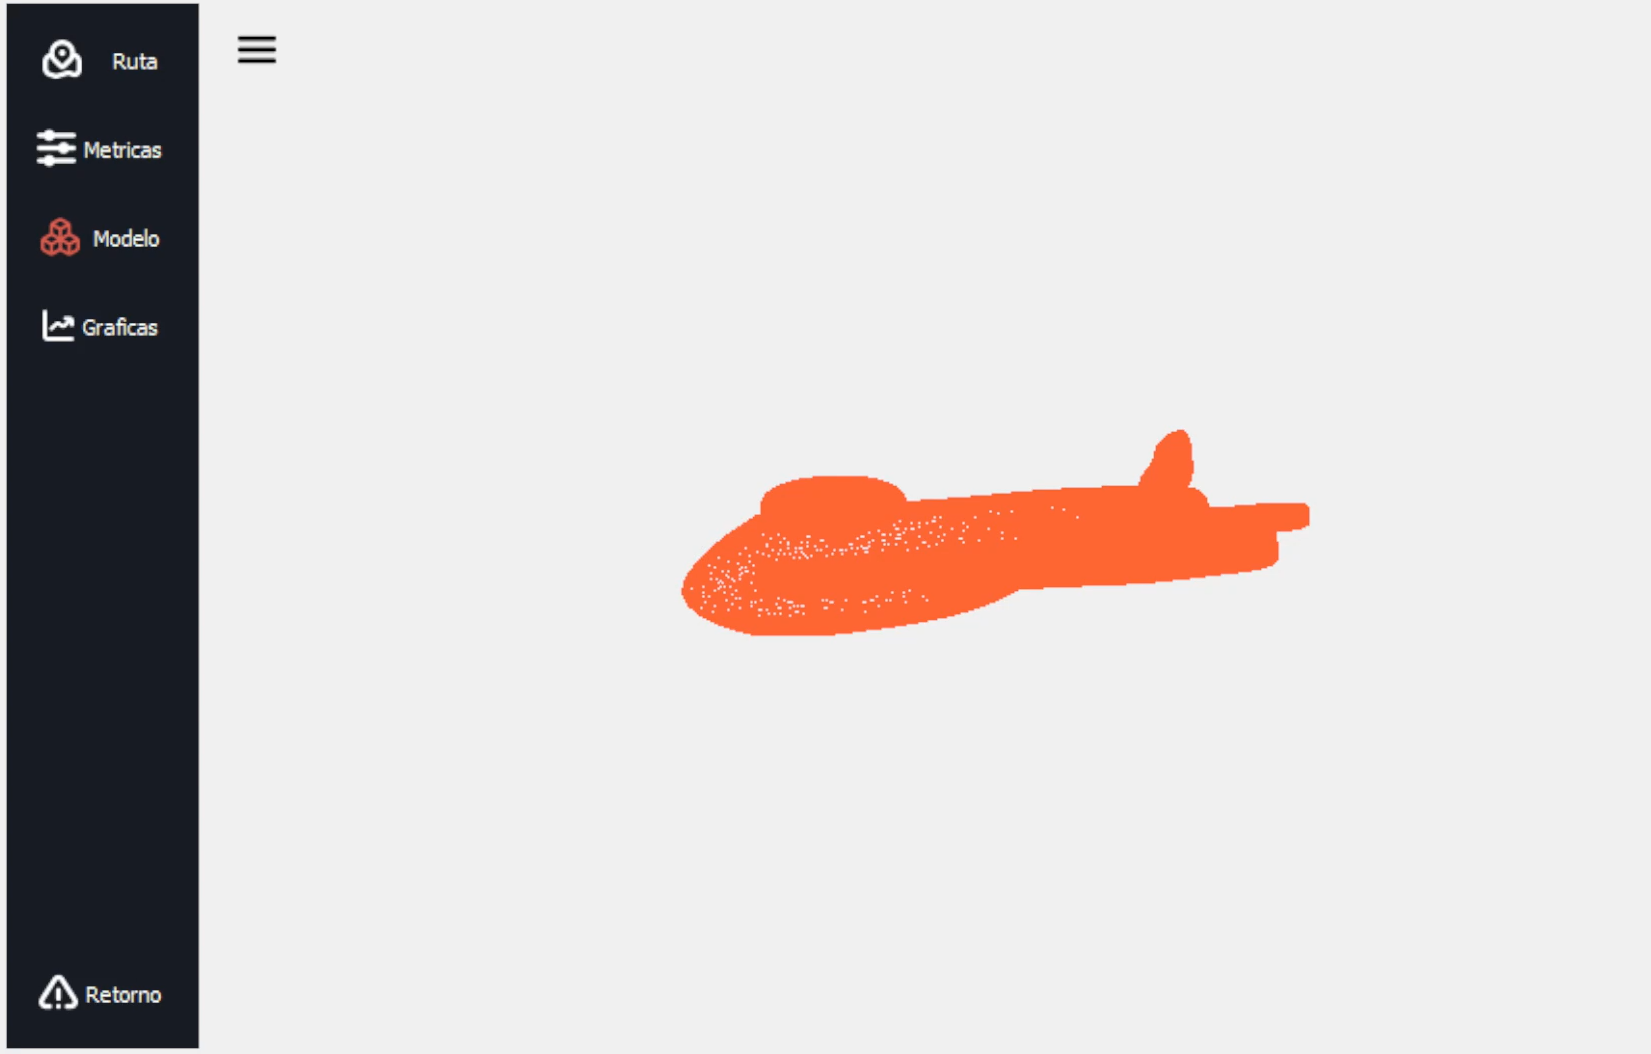
\includegraphics[width=5 in]{Imagenes/Interfaz/modelo3d.png}
    \caption{Modelo 3d UAV en la Interfaz}
    \label{fig:modelo 3d inerfaz }
\end{figure}

\subsubsection{Gráficas en Tiempo Real:}

Esta sección permite visualizar diferentes comportamientos históricos de la aeronave. Las gráficas muestran datos como movimientos inerciales (roll, pitch, yaw), altitud, temperatura, presión, y velocidad en función del tiempo. Estas gráficas son cruciales para analizar y evaluar el rendimiento del UAV durante vuelo para observar y analizar el comportamiento histórico de la aeronave.

\begin{figure}[H]
    \centering
    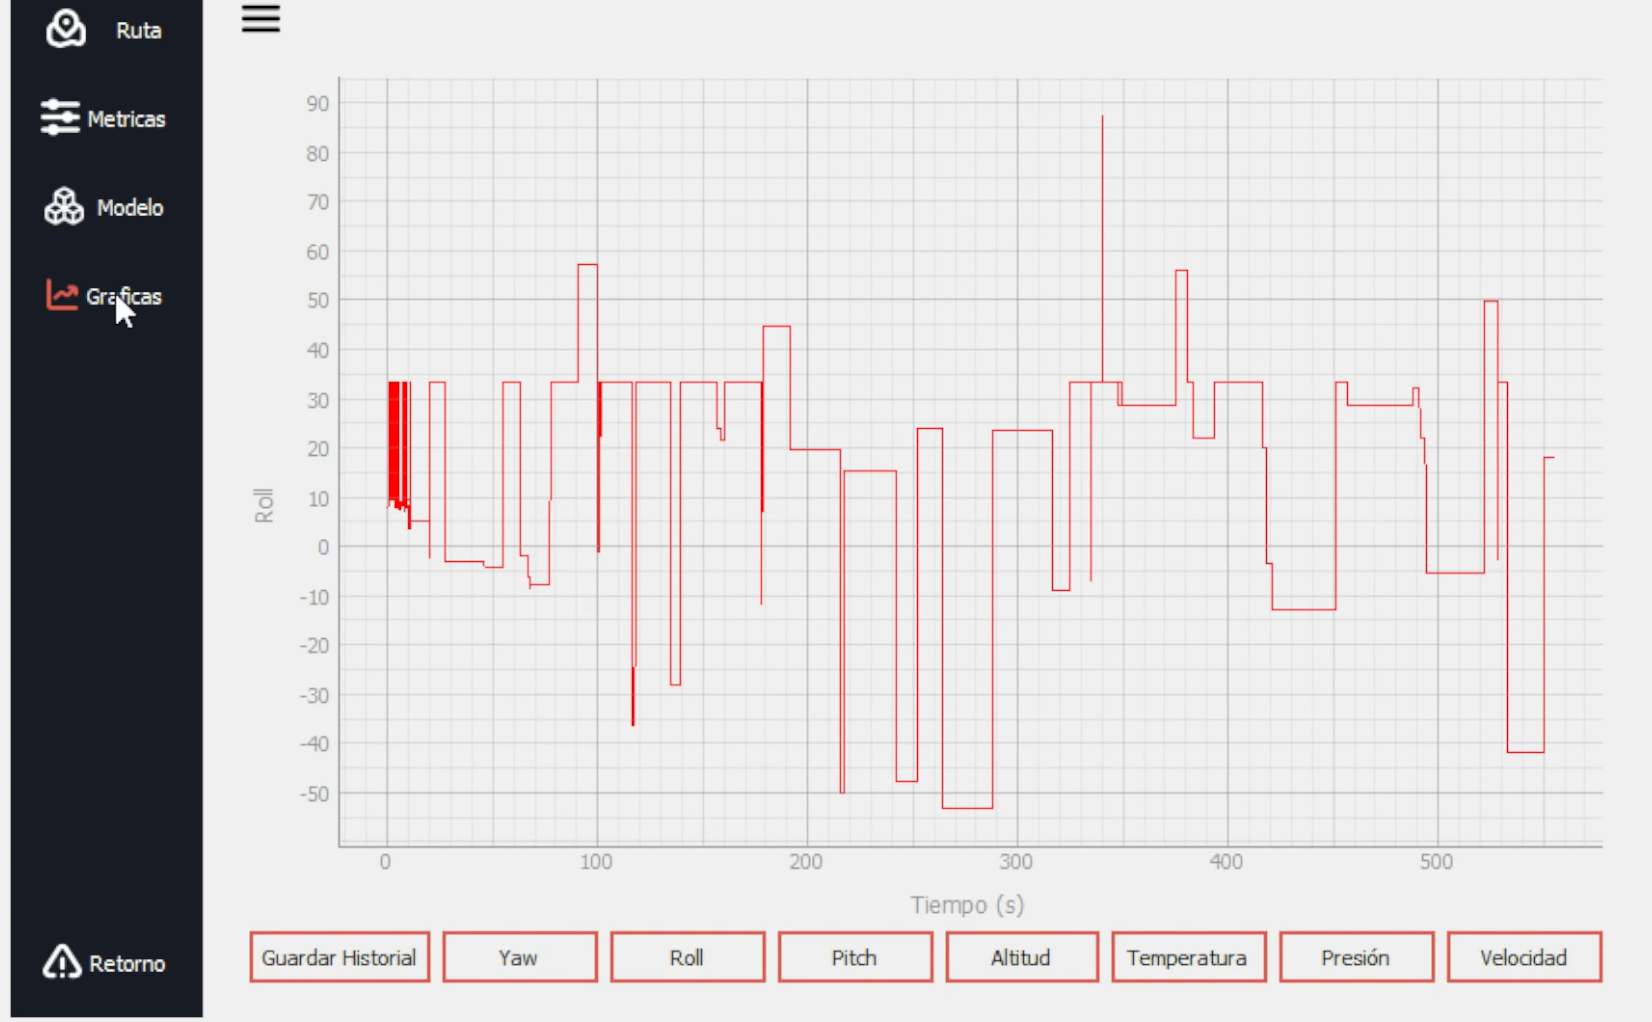
\includegraphics[width=6  in]{Imagenes/Interfaz/graficas.png}
    \caption{Gráficas de funcionamiento UAV }
    \label{fig:graficas }
\end{figure}

\clearpage
\section{Costos del Sistema}

Finalmente se hace necesario resaltar los costos asociados al desarrollo del controlador estos  se encuentran en el apartado de Anexos (véase \ref{fig:costesDesarrolloControlador}). Se resalta que el costo de los componentes electrónicos y mecánicos fue de alrededor de los \textbf{\$2'000.000}. Cabe resaltar que el desarrollo del controlador incluyendo la etapa de diseño electrónico, diseño mecánico, software, firmware y pruebas llevo alrededor de 350 horas ocasionando que el costo de desarrollo del controlador de vuelo fuera de cerca de los \textbf{\$6'4000.0000} pesos teniendo en cuenta el salario de un ingeniero electrónico promedio en Colombia que es de \textbf{ \$12.664} por hora .  

\begin{figure}[H]
    \centering
    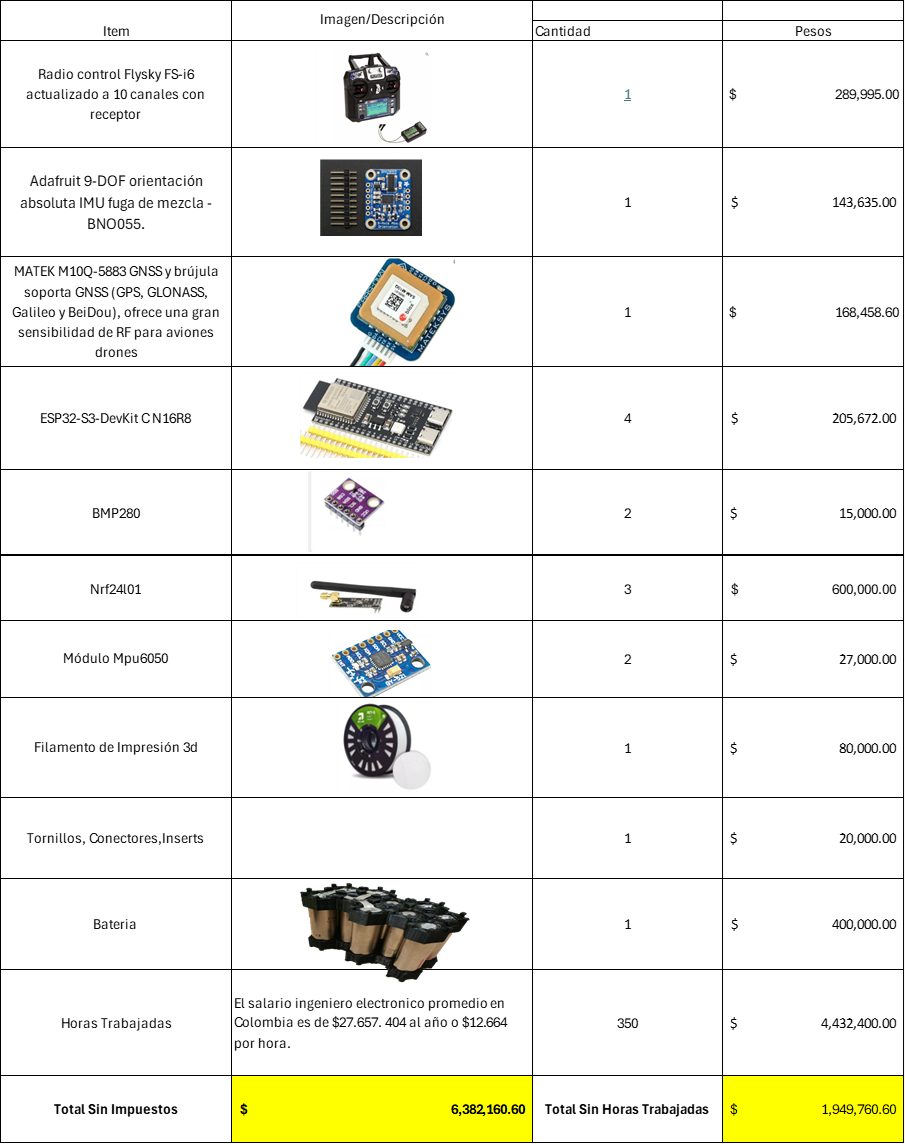
\includegraphics[width=13 cm]{Imagenes/Costos/presupuesto.png}
    \caption{Costos desarrollo Controlador }
    \label{fig:costesDesarrolloControlador}
\end{figure}
\clearpage
%\section{Pruebas de Funcionamiento}


    \subsection{Introducción}
        En esta sección se describen las pruebas realizadas para validar el funcionamiento del controlador de vuelo en conjunto. Primeramente se van a describir ciertas pruebas que se realizaron a cada sección de componentes, verificando su funcionamiento individual y la estabilidad del sistema bajo condiciones operativas.
    \subsection{Prueba de Almacenamiento de Datos}
        \vspace{5 px}
        Para este apartado de prueba de datos se utilizo el modulo de Almacenamiento de Datos que esta situado en la parte inferior del dispositivo tal y como se observa en la imagen , seguidamente se procedió a configurar la \textbf{ESP32-S3} para poder escribir y guardar datos en una unidad \textbf{microSD}. Para realizar esto, debemos recordar que la comunicación con el modulo de almacenamiento de datos se realiza mediante el protocolo \textbf{SPI} por lo que se debe instanciar los pines de \textbf{MISO, MOSI, SCK, CS} de este protocolo con los siguientes\textbf{GPIOS} :
        \vspace{5 px}
        \begin{lstlisting}[language=C++]
        #define MOSI_PIN 35
        #define SCK_PIN 36
        #define MISO_PIN 37
        #define CS_PIN 38
        \end{lstlisting}

        \vspace{5 px}

        Posteriormente, se procedió a realizar un script que fuera capaz de leer la cantidad de archivos en la unidad de almacenamiento y ponerle una cabecera de nombre que fuera \textbf{dataSaved\_n.csv} donde \textbf{n} es la cantidad de archivos que tiene la \textbf{microSD}, de tal forma que el nombre fuese único cada vez que se reinicia el dispositivo. Esto se realizo de esta forma para evitar estar sobrescribiendo información en un mismo archivo. Adicionalmente, la información que se va a guardar en la microSD, es la información crucial de todos los datos de vuelo que el UAV ha generado desde su puesta de operación hasta el momento en el que se recupere esta información. \\
        \vspace{10 px}
        Para ver la capacidad de recolección de datos del dispositivos y el tamaño del archivo generado .Se procedió a dejar simulando el dispositivo durante 3  horas y 20 minutos, generando un archivo CSV con un tamaño de 1,18 MB (1.245.184 bytes). El archivo contiene un total de 17.031 líneas de datos.


        Para estimar la capacidad de almacenamiento a largo plazo, realizamos una proyección utilizando una memoria de 64 GB. A continuación, se muestra el cálculo detallado:

        \vspace{5 px}
        \begin{itemize}
            \item Tamaño del archivo generado: 1,18 MB (1.245.184 bytes)
            \item Duración de la prueba: 3 horas y 20 minutos (3,33 horas)
            \item Número de líneas en el archivo: 17.031
        \end{itemize}
        \vspace{5 px}
        Para determinar cuántas horas de operación se pueden almacenar en una memoria de 64 GB (68.719.476.736 bytes), utilizamos la siguiente regla de tres:

        \begin{equation}
        \frac{1.245.184 \, \text{bytes}}{3,33 \, \text{horas}} = \frac{68.719.476.736 \, \text{bytes}}{x \, \text{horas}}
        \end{equation}

        Despejando \( x \):

        \begin{equation}
        x = \frac{68.719.476.736 \, \text{bytes} \times 3,33 \, \text{horas}}{1.245.184 \, \text{bytes}} = 183.816,34 \, \text{horas}
        \end{equation}

        Para convertir las horas de operación a años, usamos la relación de 1 año = 8.760 horas:

        \begin{equation}
        \frac{183.816,34 \, \text{horas}}{8.760 \, \text{horas/año}} = 20,99 \, \text{años}
        \end{equation}

        \vspace{5 px}
        Por lo tanto, se puede almacenar información en una memoria de 64 GB durante aproximadamente 183.816,34 horas o 20,99 años, considerando el ritmo de generación de datos y el tamaño de los archivos registrados en esta prueba.


    \subsection{Verificación de la lectura y escritura del valor de los servos con osciloscopio}

        Una vez configurado el apartado de lectura de los canales del transmisor \textbf{FLYSKY-I6}, se procedió a verificar que la lectura de los canales y la escritura de los valores \textbf{PWM} en la \textbf{PCA9685} se realizara correctamente. Para ello, se utilizó un osciloscopio para visualizar tanto la señal de entrada como la de salida, como se muestra en la figura (\ref{fig:pruebasPWM}).


        \begin{figure}[H]
            \centering
            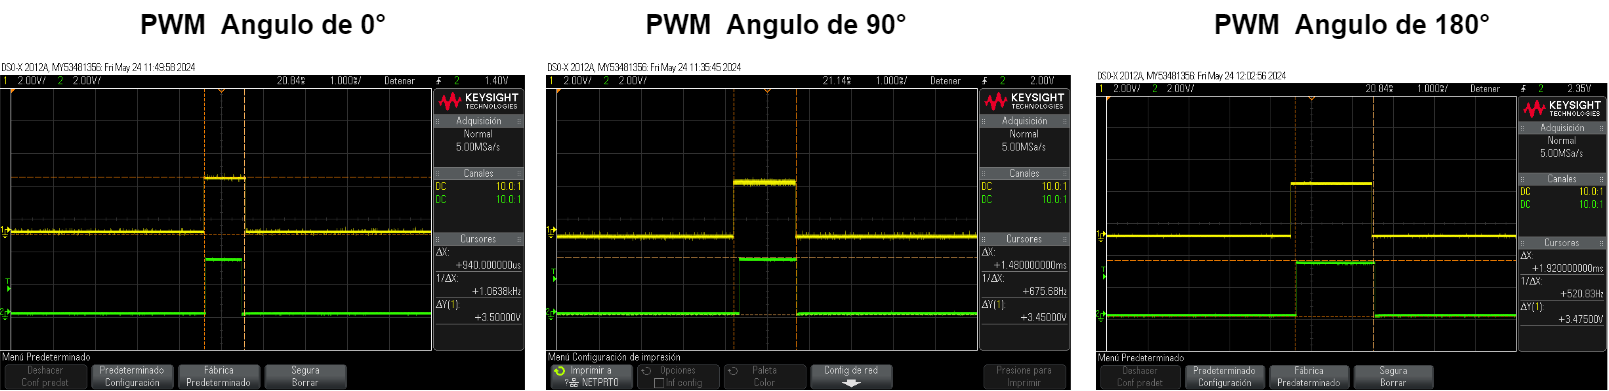
\includegraphics[width=7 in]{Imagenes/Pruebas/pwm canales.png}
            \caption{Pruebas de lectura y escritura valores PWM}
            \label{fig:pruebasPWM}
        \end{figure}

        La prueba del osciloscopio se realizó midiendo directamente en el pin de salida del receptor del canal 1 y en el pin de salida de la \textbf{PCA9685}. Los resultados mostraron que el cambio en la modulación por ancho de pulso (PWM) es proporcional al ángulo deseado, lo cual se puede evidenciar tanto en la lectura como en la escritura de los valores PWM.

        En la figura (\ref{fig:pruebasPWM}) se presentan tres capturas de pantalla del osciloscopio, que muestran las señales PWM correspondientes a ángulos de 0°, 90° y 180°. 

        \begin{itemize}
            \item En la primera imagen, se observa una señal PWM con un ángulo de 0°. La duración del pulso es de 940 $\mu$s, lo que indica la posición mínima posible.
            \item En la segunda imagen, la señal PWM corresponde a un ángulo de 90°. La duración del pulso es de 1.48 ms, indicando la posición por defecto o media del control.
            \item En la tercera imagen, la señal PWM corresponde a un ángulo de 180°. La duración del pulso es de 1.92 ms, indicando la posición máxima posible.
        \end{itemize}

        Adicionalmente, es importante señalar que en las imágenes la línea verde representa la señal del receptor, mientras que la línea amarilla representa la señal de la \textbf{PCA9685}. Estos resultados confirman que la modulación por ancho de pulso (PWM) cambia proporcionalmente con el ángulo deseado, garantizando un control preciso y predecible de los servomecanismos o actuadores conectados al sistema.
        \vspace{5 px}
    \subsection{Comparación de Controladores}
        \vspace{5 px}
        Para esta prueba, se compararon los valores de los ángulos de Roll y Pitch entre el controlador diseñado y un controlador comercial, el SpeedyBee V3 F405. Los dos controladores se situaron como se observa en la imagen y se configuraron los offsets iniciales para asegurar una medición precisa desde el mismo punto de referencia.
        \vspace{5 px}


        Para obtener los valores del controlador SpeedyBee, se utilizó la aplicación de Betaflight, la cual permite obtener los valores de Yaw, Pitch y Roll. Se contrastaron las mediciones cada diez grados de los ángulos y se puede observar en las imágenes que el comportamiento de ambos controladores es bastante similar.
        \vspace{5 px}
    \subsubsection{Descripción del SpeedyBee V3 F405}
        \vspace{5 px}
        El SpeedyBee V3 F405 es un controlador de vuelo comercial diseñado para drones. Este controlador es conocido por su estabilidad y precisión en la medición de ángulos, y es ampliamente utilizado en la comunidad de drones por su integración con la aplicación Betaflight, que facilita la configuración y obtención de datos de vuelo.
        \vspace{5 px}
        \begin{figure}[H]
            \centering
            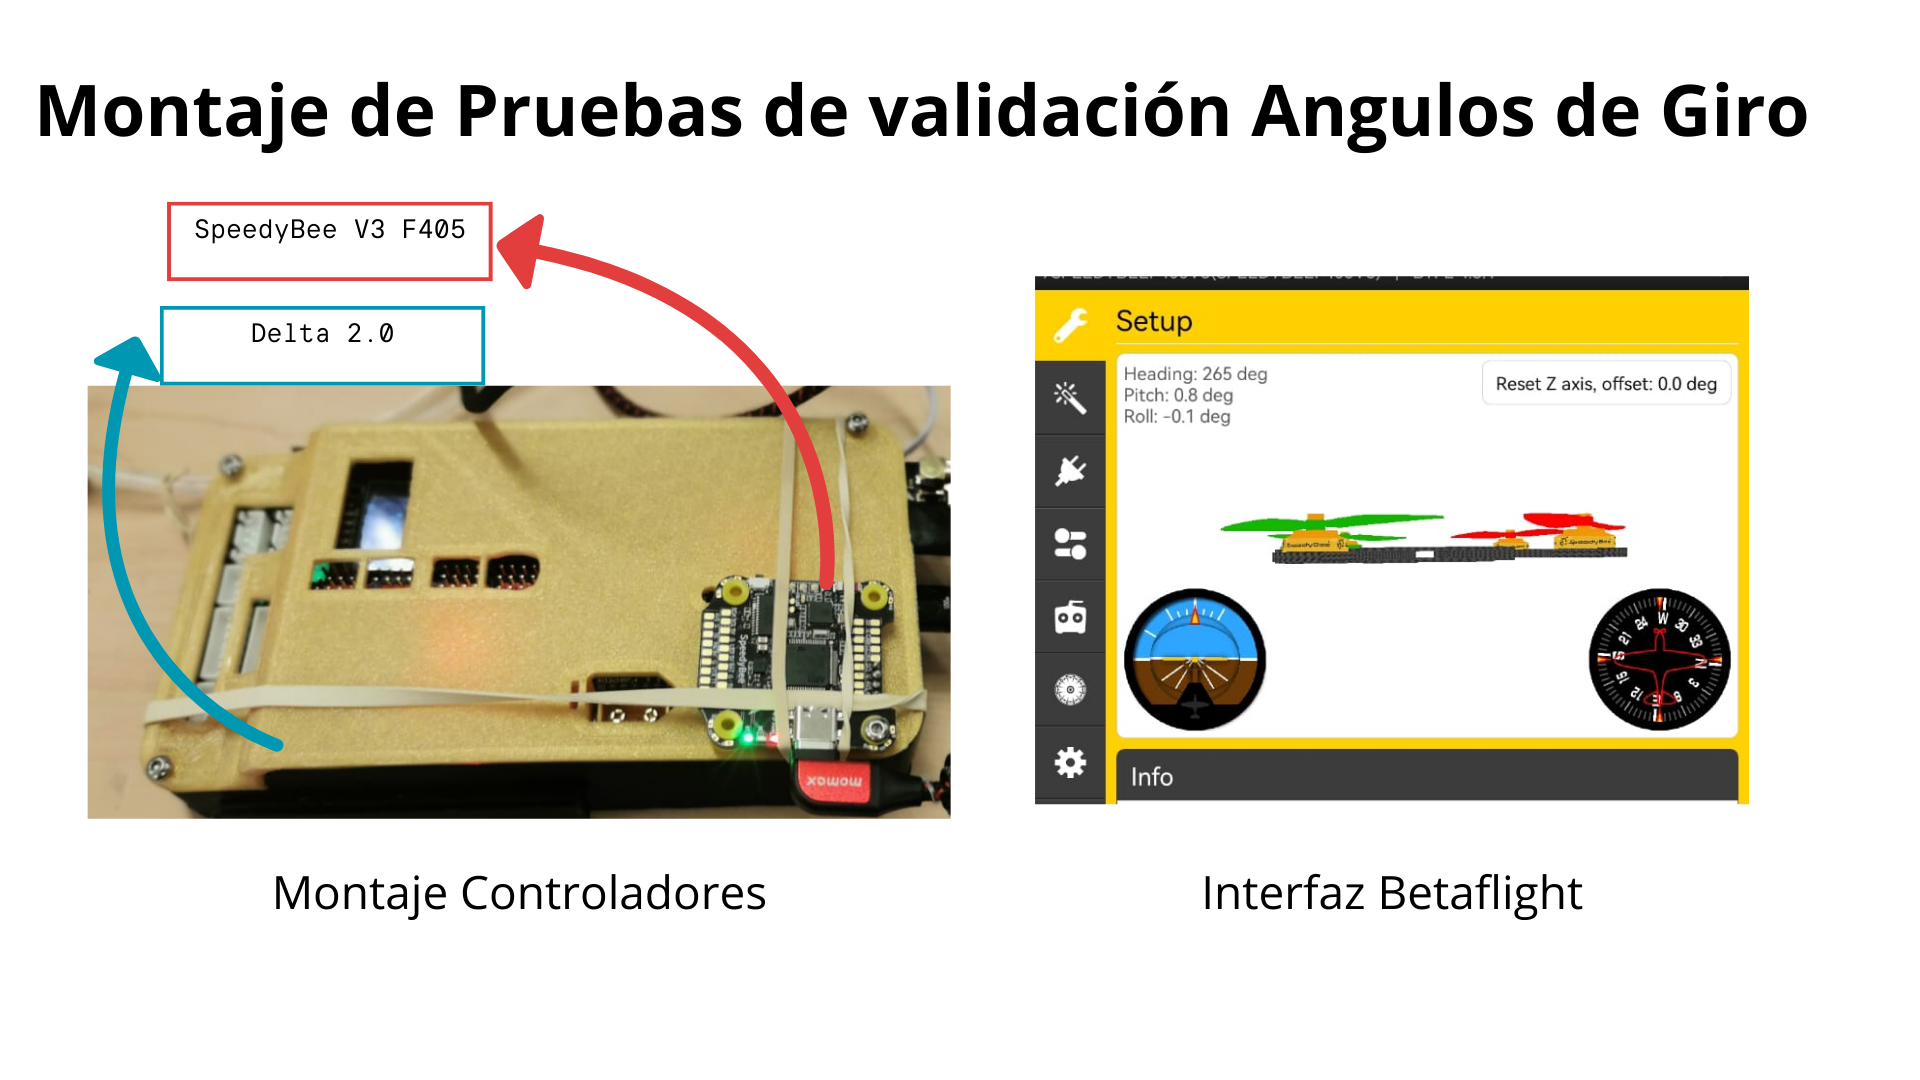
\includegraphics[width=\textwidth]{Imagenes/Pruebas/montajeControladores.png}
            \caption{Pruebas de validación y montaje controladores }
            \label{fig:pruebasPWM}
        \end{figure}



    \subsubsection{Resultados de la Prueba}



        \begin{table}[H] 
        \centering
        \caption{Toma de datos 1 y 2 para Roll}
        \resizebox{0.8\textwidth}{!}{

        \begin{tabular}{c|
        >{\columncolor[HTML]{C1F0C8}}c 
        >{\columncolor[HTML]{C1F0C8}}c 
        >{\columncolor[HTML]{C1F0C8}}c |
        >{\columncolor[HTML]{C0E6F5}}c 
        >{\columncolor[HTML]{C0E6F5}}c 
        >{\columncolor[HTML]{C0E6F5}}c |}
        \cline{2-7}
        \multicolumn{1}{l|}{}             & \multicolumn{3}{c|}{\cellcolor[HTML]{47D359}\textit{\textbf{Toma de datos 1}}}                                                                                                                                         & \multicolumn{3}{c|}{\cellcolor[HTML]{44B3E1}\textit{\textbf{Toma de datos 2}}}                                                                                                                                            \\ \hline
        \multicolumn{1}{|c|}{\textbf{X}}  & \multicolumn{1}{c|}{\cellcolor[HTML]{83E28E}\textit{\textbf{Roll SpeedyBee v3 f405}}} & \multicolumn{1}{c|}{\cellcolor[HTML]{83E28E}\textit{\textbf{Roll Delta}}} & \cellcolor[HTML]{83E28E}\textit{\textbf{\% Error}} & \multicolumn{1}{c|}{\cellcolor[HTML]{61CBF3}\textit{\textbf{Roll SpeedyBee v3 f405}}} & \multicolumn{1}{c|}{\cellcolor[HTML]{61CBF3}\textit{\textbf{Roll Delta  2}}} & \cellcolor[HTML]{61CBF3}\textit{\textbf{\% Error}} \\ \hline
        \multicolumn{1}{|c|}{\textbf{1}}  & \multicolumn{1}{c|}{\cellcolor[HTML]{C1F0C8}\textit{0}}                               & \multicolumn{1}{c|}{\cellcolor[HTML]{C1F0C8}\textit{0,44}}                & \textit{1\%}                                       & \multicolumn{1}{c|}{\cellcolor[HTML]{C0E6F5}\textit{0}}                               & \multicolumn{1}{c|}{\cellcolor[HTML]{C0E6F5}\textit{0}}                      & \textit{0}                                         \\ \hline
        \multicolumn{1}{|c|}{\textbf{2}}  & \multicolumn{1}{c|}{\cellcolor[HTML]{C1F0C8}\textit{10,3}}                            & \multicolumn{1}{c|}{\cellcolor[HTML]{C1F0C8}\textit{10,44}}               & \textit{1\%}                                       & \multicolumn{1}{c|}{\cellcolor[HTML]{C0E6F5}\textit{10,1}}                            & \multicolumn{1}{c|}{\cellcolor[HTML]{C0E6F5}\textit{10,38}}                  & \textit{3\%}                                       \\ \hline
        \multicolumn{1}{|c|}{\textbf{3}}  & \multicolumn{1}{c|}{\cellcolor[HTML]{C1F0C8}\textit{20,6}}                            & \multicolumn{1}{c|}{\cellcolor[HTML]{C1F0C8}\textit{20,2}}                & \textit{2\%}                                       & \multicolumn{1}{c|}{\cellcolor[HTML]{C0E6F5}\textit{19,5}}                            & \multicolumn{1}{c|}{\cellcolor[HTML]{C0E6F5}\textit{20,12}}                  & \textit{3\%}                                       \\ \hline
        \multicolumn{1}{|c|}{\textbf{4}}  & \multicolumn{1}{c|}{\cellcolor[HTML]{C1F0C8}\textit{31,2}}                            & \multicolumn{1}{c|}{\cellcolor[HTML]{C1F0C8}\textit{30,62}}               & \textit{2\%}                                       & \multicolumn{1}{c|}{\cellcolor[HTML]{C0E6F5}\textit{30,7}}                            & \multicolumn{1}{c|}{\cellcolor[HTML]{C0E6F5}\textit{30,69}}                  & \textit{0\%}                                       \\ \hline
        \multicolumn{1}{|c|}{\textbf{5}}  & \multicolumn{1}{c|}{\cellcolor[HTML]{C1F0C8}\textit{41,7}}                            & \multicolumn{1}{c|}{\cellcolor[HTML]{C1F0C8}\textit{40,19}}               & \textit{4\%}                                       & \multicolumn{1}{c|}{\cellcolor[HTML]{C0E6F5}\textit{40,8}}                            & \multicolumn{1}{c|}{\cellcolor[HTML]{C0E6F5}\textit{40,38}}                  & \textit{1\%}                                       \\ \hline
        \multicolumn{1}{|c|}{\textbf{6}}  & \multicolumn{1}{c|}{\cellcolor[HTML]{C1F0C8}\textit{52,1}}                            & \multicolumn{1}{c|}{\cellcolor[HTML]{C1F0C8}\textit{50,63}}               & \textit{3\%}                                       & \multicolumn{1}{c|}{\cellcolor[HTML]{C0E6F5}\textit{52}}                              & \multicolumn{1}{c|}{\cellcolor[HTML]{C0E6F5}\textit{50,25}}                  & \textit{3\%}                                       \\ \hline
        \multicolumn{1}{|c|}{\textbf{7}}  & \multicolumn{1}{c|}{\cellcolor[HTML]{C1F0C8}\textit{63,2}}                            & \multicolumn{1}{c|}{\cellcolor[HTML]{C1F0C8}\textit{60,56}}               & \textit{4\%}                                       & \multicolumn{1}{c|}{\cellcolor[HTML]{C0E6F5}\textit{61,3}}                            & \multicolumn{1}{c|}{\cellcolor[HTML]{C0E6F5}\textit{60,63}}                  & \textit{1\%}                                       \\ \hline
        \multicolumn{1}{|c|}{\textbf{8}}  & \multicolumn{1}{c|}{\cellcolor[HTML]{C1F0C8}\textit{72,8}}                            & \multicolumn{1}{c|}{\cellcolor[HTML]{C1F0C8}\textit{70,5}}                & \textit{3\%}                                       & \multicolumn{1}{c|}{\cellcolor[HTML]{C0E6F5}\textit{73,2}}                            & \multicolumn{1}{c|}{\cellcolor[HTML]{C0E6F5}\textit{70,12}}                  & \textit{4\%}                                       \\ \hline
        \multicolumn{1}{|c|}{\textbf{9}}  & \multicolumn{1}{c|}{\cellcolor[HTML]{C1F0C8}\textit{83,1}}                            & \multicolumn{1}{c|}{\cellcolor[HTML]{C1F0C8}\textit{80,56}}               & \textit{3\%}                                       & \multicolumn{1}{c|}{\cellcolor[HTML]{C0E6F5}\textit{84,2}}                            & \multicolumn{1}{c|}{\cellcolor[HTML]{C0E6F5}\textit{80,44}}                  & \textit{4\%}                                       \\ \hline
        \multicolumn{1}{|c|}{\textbf{10}} & \multicolumn{1}{c|}{\cellcolor[HTML]{C1F0C8}\textit{86,5}}                            & \multicolumn{1}{c|}{\cellcolor[HTML]{C1F0C8}\textit{87,1}}                & \textit{1\%}                                       & \multicolumn{1}{c|}{\cellcolor[HTML]{C0E6F5}\textit{92,9}}                            & \multicolumn{1}{c|}{\cellcolor[HTML]{C0E6F5}\textit{88,44}}                  & \textit{5\%}                                       \\ \hline
        \multicolumn{1}{|c|}{\textbf{11}} & \multicolumn{1}{c|}{\cellcolor[HTML]{C1F0C8}\textit{-8,7}}                            & \multicolumn{1}{c|}{\cellcolor[HTML]{C1F0C8}\textit{-10,38}}              & \textit{19\%}                                      & \multicolumn{1}{c|}{\cellcolor[HTML]{C0E6F5}\textit{-9,6}}                            & \multicolumn{1}{c|}{\cellcolor[HTML]{C0E6F5}\textit{-10,56}}                 & \textit{10\%}                                      \\ \hline
        \multicolumn{1}{|c|}{\textbf{12}} & \multicolumn{1}{c|}{\cellcolor[HTML]{C1F0C8}\textit{-19,8}}                           & \multicolumn{1}{c|}{\cellcolor[HTML]{C1F0C8}\textit{-20,31}}              & \textit{3\%}                                       & \multicolumn{1}{c|}{\cellcolor[HTML]{C0E6F5}\textit{-19,1}}                           & \multicolumn{1}{c|}{\cellcolor[HTML]{C0E6F5}\textit{-20,25}}                 & \textit{6\%}                                       \\ \hline
        \multicolumn{1}{|c|}{\textbf{13}} & \multicolumn{1}{c|}{\cellcolor[HTML]{C1F0C8}\textit{-30}}                             & \multicolumn{1}{c|}{\cellcolor[HTML]{C1F0C8}\textit{-30,19}}              & \textit{1\%}                                       & \multicolumn{1}{c|}{\cellcolor[HTML]{C0E6F5}\textit{-29,4}}                           & \multicolumn{1}{c|}{\cellcolor[HTML]{C0E6F5}\textit{-30,25}}                 & \textit{3\%}                                       \\ \hline
        \multicolumn{1}{|c|}{\textbf{14}} & \multicolumn{1}{c|}{\cellcolor[HTML]{C1F0C8}\textit{-40,7}}                           & \multicolumn{1}{c|}{\cellcolor[HTML]{C1F0C8}\textit{-39,1}}               & \textit{4\%}                                       & \multicolumn{1}{c|}{\cellcolor[HTML]{C0E6F5}\textit{-39,1}}                           & \multicolumn{1}{c|}{\cellcolor[HTML]{C0E6F5}\textit{-40,13}}                 & \textit{3\%}                                       \\ \hline
        \multicolumn{1}{|c|}{\textbf{15}} & \multicolumn{1}{c|}{\cellcolor[HTML]{C1F0C8}\textit{-50,9}}                           & \multicolumn{1}{c|}{\cellcolor[HTML]{C1F0C8}\textit{-50,63}}              & \textit{1\%}                                       & \multicolumn{1}{c|}{\cellcolor[HTML]{C0E6F5}\textit{-49,2}}                           & \multicolumn{1}{c|}{\cellcolor[HTML]{C0E6F5}\textit{-50,88}}                 & \textit{3\%}                                       \\ \hline
        \multicolumn{1}{|c|}{\textbf{16}} & \multicolumn{1}{c|}{\cellcolor[HTML]{C1F0C8}\textit{-59,8}}                           & \multicolumn{1}{c|}{\cellcolor[HTML]{C1F0C8}\textit{-60,25}}              & \textit{1\%}                                       & \multicolumn{1}{c|}{\cellcolor[HTML]{C0E6F5}\textit{-59,5}}                           & \multicolumn{1}{c|}{\cellcolor[HTML]{C0E6F5}\textit{-60,75}}                 & \textit{2\%}                                       \\ \hline
        \multicolumn{1}{|c|}{\textbf{17}} & \multicolumn{1}{c|}{\cellcolor[HTML]{C1F0C8}\textit{-69,7}}                           & \multicolumn{1}{c|}{\cellcolor[HTML]{C1F0C8}\textit{-70,37}}              & \textit{1\%}                                       & \multicolumn{1}{c|}{\cellcolor[HTML]{C0E6F5}\textit{-67,8}}                           & \multicolumn{1}{c|}{\cellcolor[HTML]{C0E6F5}\textit{-70,19}}                 & \textit{4\%}                                       \\ \hline
        \multicolumn{1}{|c|}{\textbf{18}} & \multicolumn{1}{c|}{\cellcolor[HTML]{C1F0C8}\textit{-80,1}}                           & \multicolumn{1}{c|}{\cellcolor[HTML]{C1F0C8}\textit{-80,69}}              & \textit{1\%}                                       & \multicolumn{1}{c|}{\cellcolor[HTML]{C0E6F5}\textit{-77,9}}                           & \multicolumn{1}{c|}{\cellcolor[HTML]{C0E6F5}\textit{-80,81}}                 & \textit{4\%}                                       \\ \hline
        \multicolumn{1}{|c|}{\textbf{19}} & \multicolumn{1}{c|}{\cellcolor[HTML]{C1F0C8}\textit{-89,2}}                           & \multicolumn{1}{c|}{\cellcolor[HTML]{C1F0C8}\textit{-90,06}}              & \textit{1\%}                                       & \multicolumn{1}{c|}{\cellcolor[HTML]{C0E6F5}\textit{-87,3}}                           & \multicolumn{1}{c|}{\cellcolor[HTML]{C0E6F5}\textit{-90,06}}                 & \textit{3\%}                                       \\ \hline
        \end{tabular}
        }

        \end{table}



        % Please add the following required packages to your document preamble:
        % \usepackage[table,xcdraw]{xcolor}
        % Beamer presentation requires \usepackage{colortbl} instead of \usepackage[table,xcdraw]{xcolor}
        \begin{table}[H] 

        \centering
        \caption{Toma de datos 1 y 2 para Pitch}
        \resizebox{0.8\textwidth}{!}{

        \begin{tabular}{c|
        >{\columncolor[HTML]{F2CEEF}}c 
        >{\columncolor[HTML]{F2CEEF}}c 
        >{\columncolor[HTML]{F2CEEF}}c |
        >{\columncolor[HTML]{CCCCFF}}c 
        >{\columncolor[HTML]{CCCCFF}}c 
        >{\columncolor[HTML]{CCCCFF}}c |}
        \cline{2-7}
        \multicolumn{1}{l|}{}             & \multicolumn{3}{c|}{\cellcolor[HTML]{D86DCD}\textbf{Toma de datos 1}}                                                                                                                          & \multicolumn{3}{c|}{\cellcolor[HTML]{6666FF}\textbf{Toma de datos 2}}                                                                                                                            \\ \hline
        \multicolumn{1}{|c|}{\textbf{X}}  & \multicolumn{1}{c|}{\cellcolor[HTML]{E49EDD}\textbf{Pitch  SpeedyBee v3 f405}} & \multicolumn{1}{c|}{\cellcolor[HTML]{E49EDD}\textbf{Pitch Delta}} & \cellcolor[HTML]{E49EDD}\textbf{\% Error} & \multicolumn{1}{c|}{\cellcolor[HTML]{9999FF}\textbf{Pitch  SpeedyBee v3 f405}} & \multicolumn{1}{c|}{\cellcolor[HTML]{9999FF}\textbf{Pitch Delta 2}} & \cellcolor[HTML]{9999FF}\textbf{\% Error} \\ \hline
        \multicolumn{1}{|c|}{\textbf{1}}  & \multicolumn{1}{c|}{\cellcolor[HTML]{F2CEEF}0}                                 & \multicolumn{1}{c|}{\cellcolor[HTML]{F2CEEF}-0,44}                & 1\%                                       & \multicolumn{1}{c|}{\cellcolor[HTML]{CCCCFF}0,1}                               & \multicolumn{1}{c|}{\cellcolor[HTML]{CCCCFF}0,94}                   & 0\%                                       \\ \hline
        \multicolumn{1}{|c|}{\textbf{2}}  & \multicolumn{1}{c|}{\cellcolor[HTML]{F2CEEF}10,8}                              & \multicolumn{1}{c|}{\cellcolor[HTML]{F2CEEF}10,6}                 & 2\%                                       & \multicolumn{1}{c|}{\cellcolor[HTML]{CCCCFF}10,8}                              & \multicolumn{1}{c|}{\cellcolor[HTML]{CCCCFF}10,44}                  & 3\%                                       \\ \hline
        \multicolumn{1}{|c|}{\textbf{3}}  & \multicolumn{1}{c|}{\cellcolor[HTML]{F2CEEF}21,6}                              & \multicolumn{1}{c|}{\cellcolor[HTML]{F2CEEF}20,12}                & 7\%                                       & \multicolumn{1}{c|}{\cellcolor[HTML]{CCCCFF}19,8}                              & \multicolumn{1}{c|}{\cellcolor[HTML]{CCCCFF}20}                     & 1\%                                       \\ \hline
        \multicolumn{1}{|c|}{\textbf{4}}  & \multicolumn{1}{c|}{\cellcolor[HTML]{F2CEEF}31,9}                              & \multicolumn{1}{c|}{\cellcolor[HTML]{F2CEEF}30,44}                & 5\%                                       & \multicolumn{1}{c|}{\cellcolor[HTML]{CCCCFF}30,1}                              & \multicolumn{1}{c|}{\cellcolor[HTML]{CCCCFF}30,31}                  & 1\%                                       \\ \hline
        \multicolumn{1}{|c|}{\textbf{5}}  & \multicolumn{1}{c|}{\cellcolor[HTML]{F2CEEF}41,9}                              & \multicolumn{1}{c|}{\cellcolor[HTML]{F2CEEF}40,13}                & 4\%                                       & \multicolumn{1}{c|}{\cellcolor[HTML]{CCCCFF}40,8}                              & \multicolumn{1}{c|}{\cellcolor[HTML]{CCCCFF}40,63}                  & 0\%                                       \\ \hline
        \multicolumn{1}{|c|}{\textbf{6}}  & \multicolumn{1}{c|}{\cellcolor[HTML]{F2CEEF}53,2}                              & \multicolumn{1}{c|}{\cellcolor[HTML]{F2CEEF}50,63}                & 5\%                                       & \multicolumn{1}{c|}{\cellcolor[HTML]{CCCCFF}50,1}                              & \multicolumn{1}{c|}{\cellcolor[HTML]{CCCCFF}50,19}                  & 0\%                                       \\ \hline
        \multicolumn{1}{|c|}{\textbf{7}}  & \multicolumn{1}{c|}{\cellcolor[HTML]{F2CEEF}63,5}                              & \multicolumn{1}{c|}{\cellcolor[HTML]{F2CEEF}60,96}                & 4\%                                       & \multicolumn{1}{c|}{\cellcolor[HTML]{CCCCFF}60,9}                              & \multicolumn{1}{c|}{\cellcolor[HTML]{CCCCFF}60,19}                  & 1\%                                       \\ \hline
        \multicolumn{1}{|c|}{\textbf{8}}  & \multicolumn{1}{c|}{\cellcolor[HTML]{F2CEEF}73,3}                              & \multicolumn{1}{c|}{\cellcolor[HTML]{F2CEEF}70,75}                & 3\%                                       & \multicolumn{1}{c|}{\cellcolor[HTML]{CCCCFF}71,5}                              & \multicolumn{1}{c|}{\cellcolor[HTML]{CCCCFF}70,44}                  & 1\%                                       \\ \hline
        \multicolumn{1}{|c|}{\textbf{9}}  & \multicolumn{1}{c|}{\cellcolor[HTML]{F2CEEF}83,3}                              & \multicolumn{1}{c|}{\cellcolor[HTML]{F2CEEF}80,12}                & 4\%                                       & \multicolumn{1}{c|}{\cellcolor[HTML]{CCCCFF}82,5}                              & \multicolumn{1}{c|}{\cellcolor[HTML]{CCCCFF}80,37}                  & 3\%                                       \\ \hline
        \multicolumn{1}{|c|}{\textbf{10}} & \multicolumn{1}{c|}{\cellcolor[HTML]{F2CEEF}86,3}                              & \multicolumn{1}{c|}{\cellcolor[HTML]{F2CEEF}87,06}                & 1\%                                       & \multicolumn{1}{c|}{\cellcolor[HTML]{CCCCFF}87,5}                              & \multicolumn{1}{c|}{\cellcolor[HTML]{CCCCFF}88}                     & 1\%                                       \\ \hline
        \multicolumn{1}{|c|}{\textbf{11}} & \multicolumn{1}{c|}{\cellcolor[HTML]{F2CEEF}-9,6}                              & \multicolumn{1}{c|}{\cellcolor[HTML]{F2CEEF}-10,38}               & 8\%                                       & \multicolumn{1}{c|}{\cellcolor[HTML]{CCCCFF}-11,8}                             & \multicolumn{1}{c|}{\cellcolor[HTML]{CCCCFF}-10,13}                 & 14\%                                      \\ \hline
        \multicolumn{1}{|c|}{\textbf{12}} & \multicolumn{1}{c|}{\cellcolor[HTML]{F2CEEF}-20,5}                             & \multicolumn{1}{c|}{\cellcolor[HTML]{F2CEEF}-20,31}               & 1\%                                       & \multicolumn{1}{c|}{\cellcolor[HTML]{CCCCFF}-21,9}                             & \multicolumn{1}{c|}{\cellcolor[HTML]{CCCCFF}-20,81}                 & 5\%                                       \\ \hline
        \multicolumn{1}{|c|}{\textbf{13}} & \multicolumn{1}{c|}{\cellcolor[HTML]{F2CEEF}-29,6}                             & \multicolumn{1}{c|}{\cellcolor[HTML]{F2CEEF}-30,5}                & 3\%                                       & \multicolumn{1}{c|}{\cellcolor[HTML]{CCCCFF}-32,1}                             & \multicolumn{1}{c|}{\cellcolor[HTML]{CCCCFF}-30,44}                 & 5\%                                       \\ \hline
        \multicolumn{1}{|c|}{\textbf{14}} & \multicolumn{1}{c|}{\cellcolor[HTML]{F2CEEF}-40}                               & \multicolumn{1}{c|}{\cellcolor[HTML]{F2CEEF}-40,31}               & 1\%                                       & \multicolumn{1}{c|}{\cellcolor[HTML]{CCCCFF}-43,6}                             & \multicolumn{1}{c|}{\cellcolor[HTML]{CCCCFF}-40,75}                 & 7\%                                       \\ \hline
        \multicolumn{1}{|c|}{\textbf{15}} & \multicolumn{1}{c|}{\cellcolor[HTML]{F2CEEF}-49,2}                             & \multicolumn{1}{c|}{\cellcolor[HTML]{F2CEEF}-50,19}               & 2\%                                       & \multicolumn{1}{c|}{\cellcolor[HTML]{CCCCFF}-53,5}                             & \multicolumn{1}{c|}{\cellcolor[HTML]{CCCCFF}-50,44}                 & 6\%                                       \\ \hline
        \multicolumn{1}{|c|}{\textbf{16}} & \multicolumn{1}{c|}{\cellcolor[HTML]{F2CEEF}-58,3}                             & \multicolumn{1}{c|}{\cellcolor[HTML]{F2CEEF}-60,13}               & 3\%                                       & \multicolumn{1}{c|}{\cellcolor[HTML]{CCCCFF}-62,6}                             & \multicolumn{1}{c|}{\cellcolor[HTML]{CCCCFF}-60,75}                 & 3\%                                       \\ \hline
        \multicolumn{1}{|c|}{\textbf{17}} & \multicolumn{1}{c|}{\cellcolor[HTML]{F2CEEF}-69}                               & \multicolumn{1}{c|}{\cellcolor[HTML]{F2CEEF}-70,25}               & 2\%                                       & \multicolumn{1}{c|}{\cellcolor[HTML]{CCCCFF}-72,1}                             & \multicolumn{1}{c|}{\cellcolor[HTML]{CCCCFF}-70,5}                  & 2\%                                       \\ \hline
        \multicolumn{1}{|c|}{\textbf{18}} & \multicolumn{1}{c|}{\cellcolor[HTML]{F2CEEF}-78,9}                             & \multicolumn{1}{c|}{\cellcolor[HTML]{F2CEEF}-80,44}               & 2\%                                       & \multicolumn{1}{c|}{\cellcolor[HTML]{CCCCFF}-82,1}                             & \multicolumn{1}{c|}{\cellcolor[HTML]{CCCCFF}-80,62}                 & 2\%                                       \\ \hline
        \multicolumn{1}{|c|}{\textbf{19}} & \multicolumn{1}{c|}{\cellcolor[HTML]{F2CEEF}-87,5}                             & \multicolumn{1}{c|}{\cellcolor[HTML]{F2CEEF}-89,44}               & 2\%                                       & \multicolumn{1}{c|}{\cellcolor[HTML]{CCCCFF}-86,6}                             & \multicolumn{1}{c|}{\cellcolor[HTML]{CCCCFF}-87,19}                 & 1\%                                       \\ \hline
        \end{tabular}
        }
        \end{table}

        \subsubsection{Análisis de las Tablas}

            En las tablas de datos de Roll y Pitch, se observa que ambos controladores presentan comportamientos bastante similares. El error relativo entre las mediciones de los controladores Delta y SpeedyBee V3 F405 varía generalmente entre el 1\% y el 4\%. Sin embargo, hay excepciones notables, como cuando se miden ángulos cercanos a los -10°, tanto en Roll como en Pitch, donde el error puede llegar hasta el 19\%.

            \vspace{5px}
            Es importante destacar que existe cierta incertidumbre asociada a la forma en que se recopilaron los datos. Fijar los ángulos en diferentes grados puede introducir variaciones en las lecturas de ambos controladores debido a pequeñas discrepancias en la posición exacta y la respuesta de los sensores. Esto puede afectar la precisión de las mediciones comparadas.
            \vspace{5px}

        \subsubsection{Comparación de Roll}
            En los gráficos de la Figura \ref{fig:comparacionRoll}, se puede observar que los ángulos de Roll medidos por ambos controladores son muy similares. En la primera toma de datos, los valores siguen una tendencia casi idéntica, con variaciones mínimas en algunos puntos. En la segunda toma de datos, se observa un comportamiento similar, reafirmando la consistencia entre las mediciones de ambos dispositivos.
            \begin{figure}[H]
                \centering
                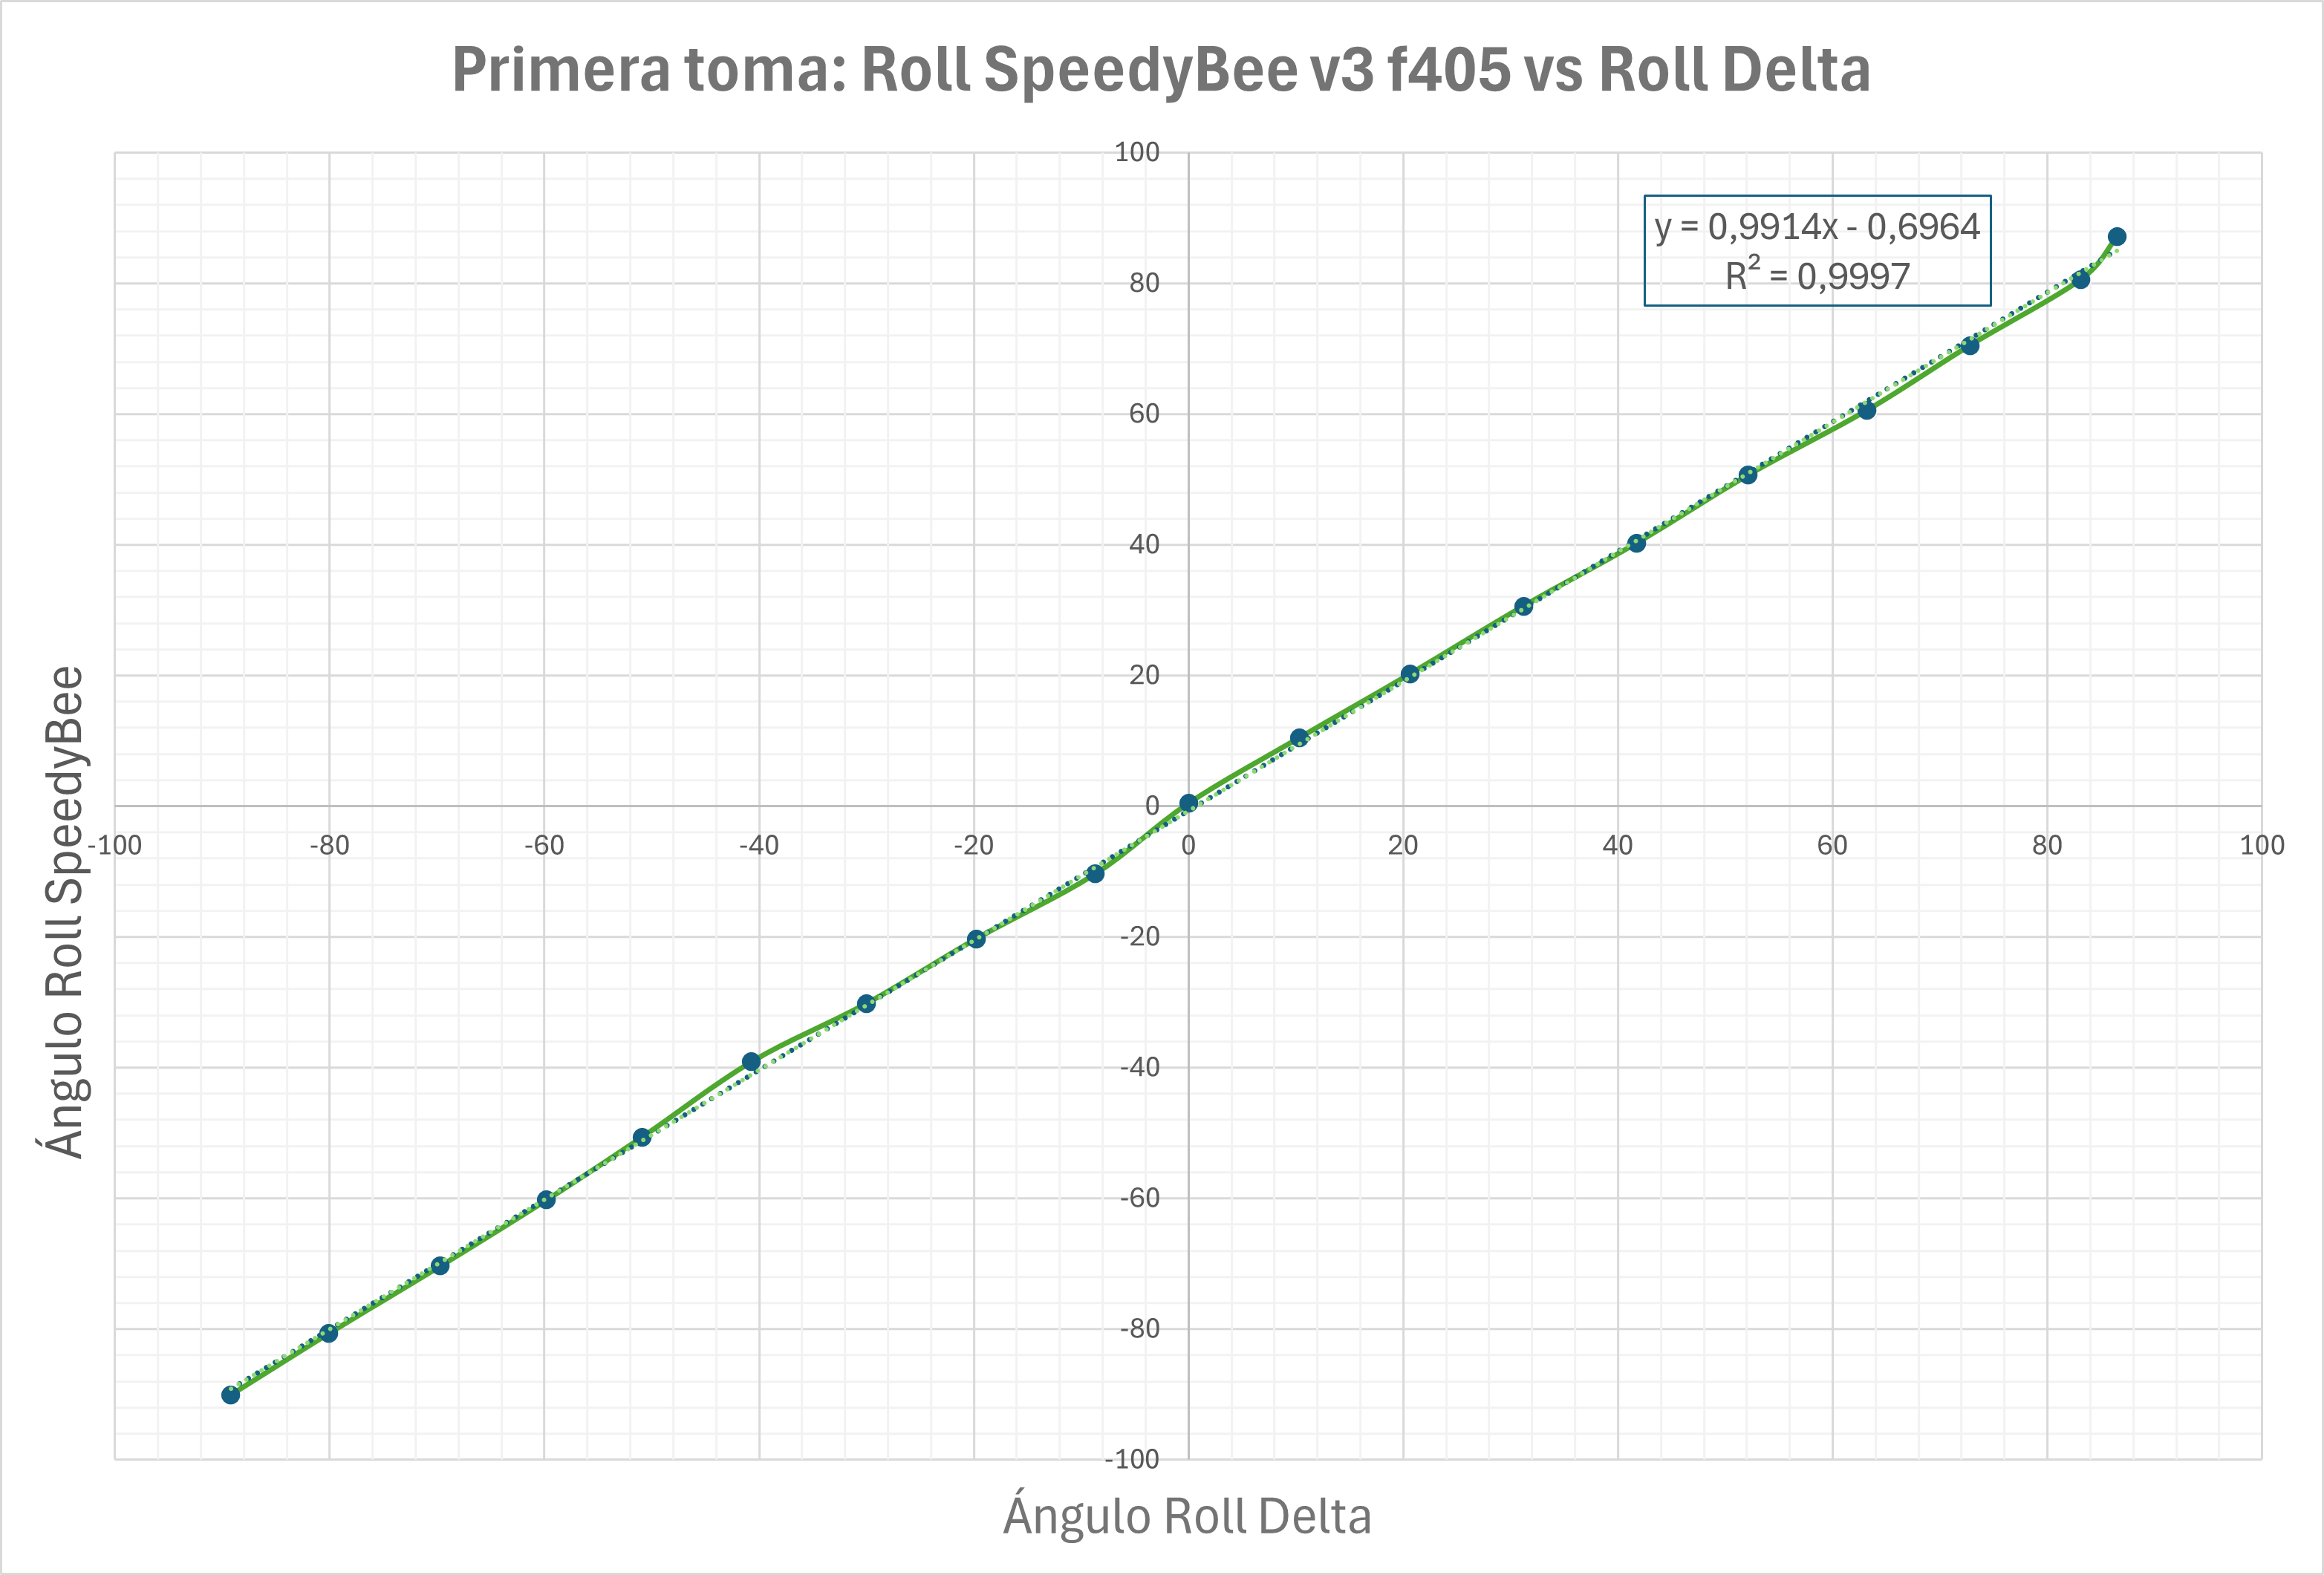
\includegraphics[width=5.5 in]{Imagenes/Pruebas/roll_1_compare.png}
                \caption{Comparación de ángulo Roll entre controladores Delta y SpeedyBee V3 F405 en la primera toma de datos }
                \label{fig:comparacionRoll}
            \end{figure}

            \begin{figure}[H]
                \centering
                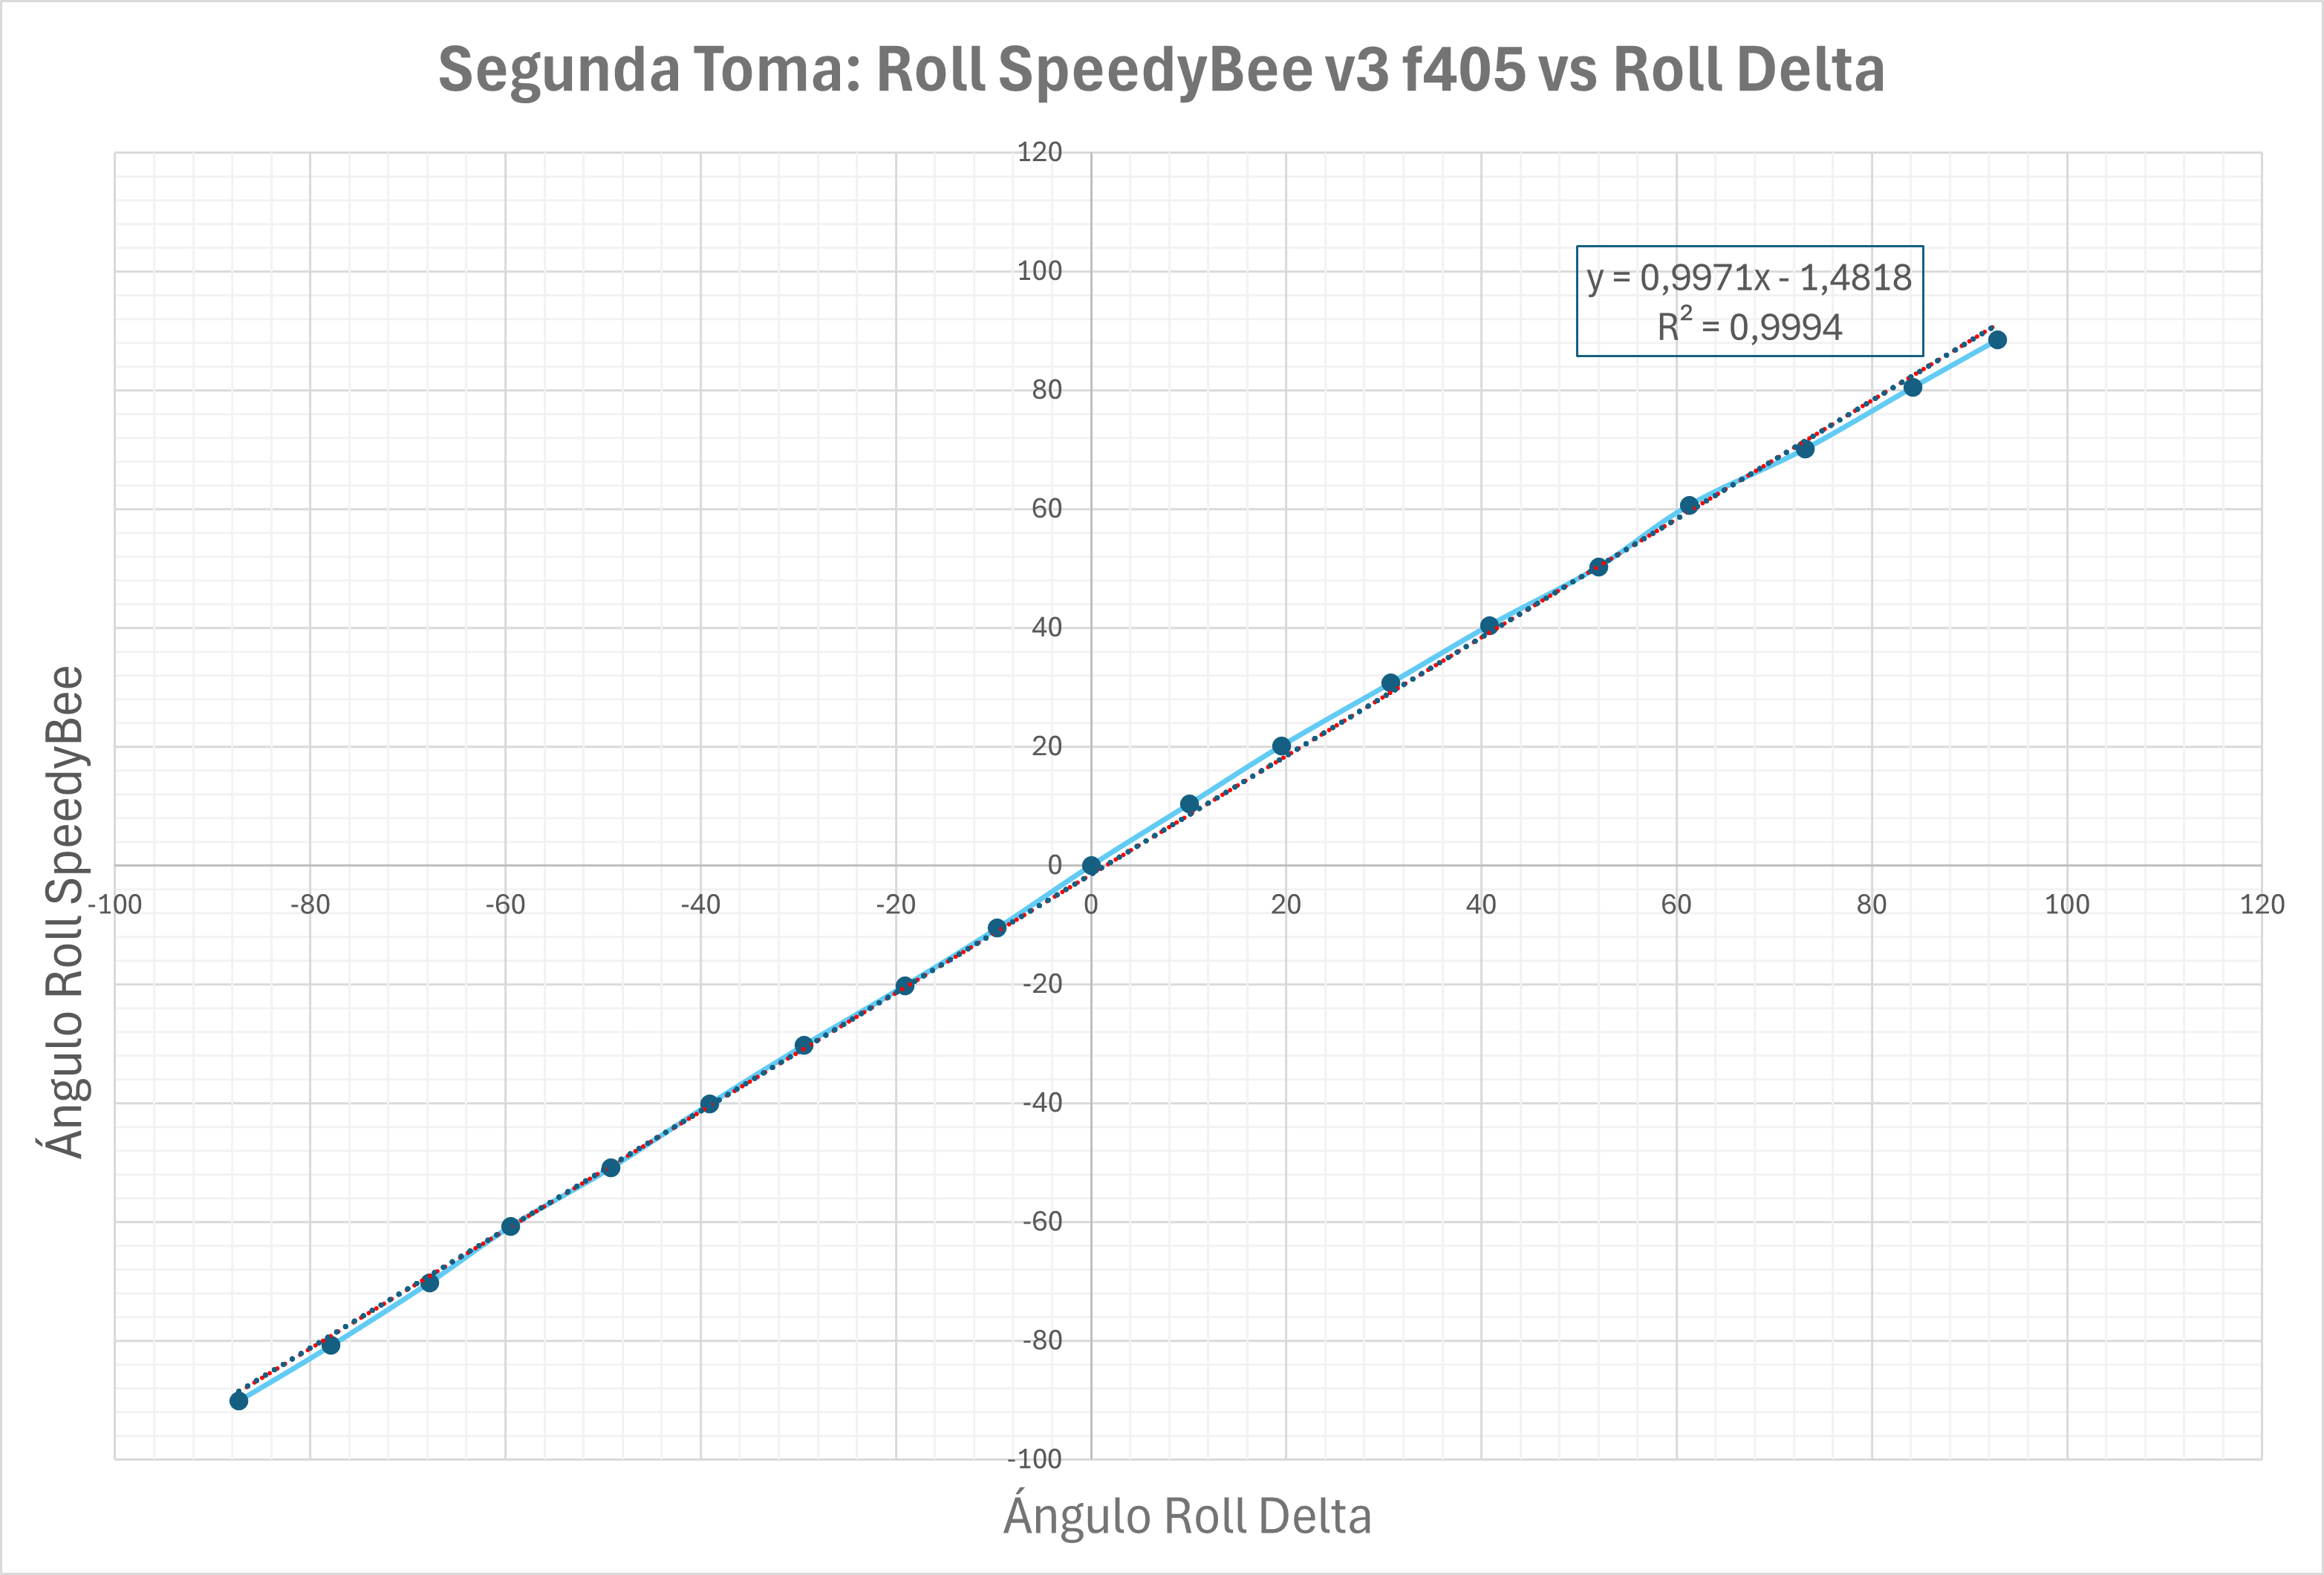
\includegraphics[width=5.5 in]{Imagenes/Pruebas/roll_2_compare.png}
                \caption{Comparación de Roll entre controladores Delta y SpeedyBee V3 F405 en la segunda toma de datos }
                \label{fig:comparacionRoll}
            \end{figure}


        \subsubsection{Comparación de Pitch}
            De manera similar, los gráficos de la Figura \ref{fig:comparacionPitch1} presentan la comparación de los ángulos de Pitch. Aquí también se evidencia que ambos controladores tienen un comportamiento muy parecido. Las diferencias entre los valores son mínimas y generalmente se mantienen dentro de un margen de error aceptable.


            \begin{figure}[H]
                \centering
                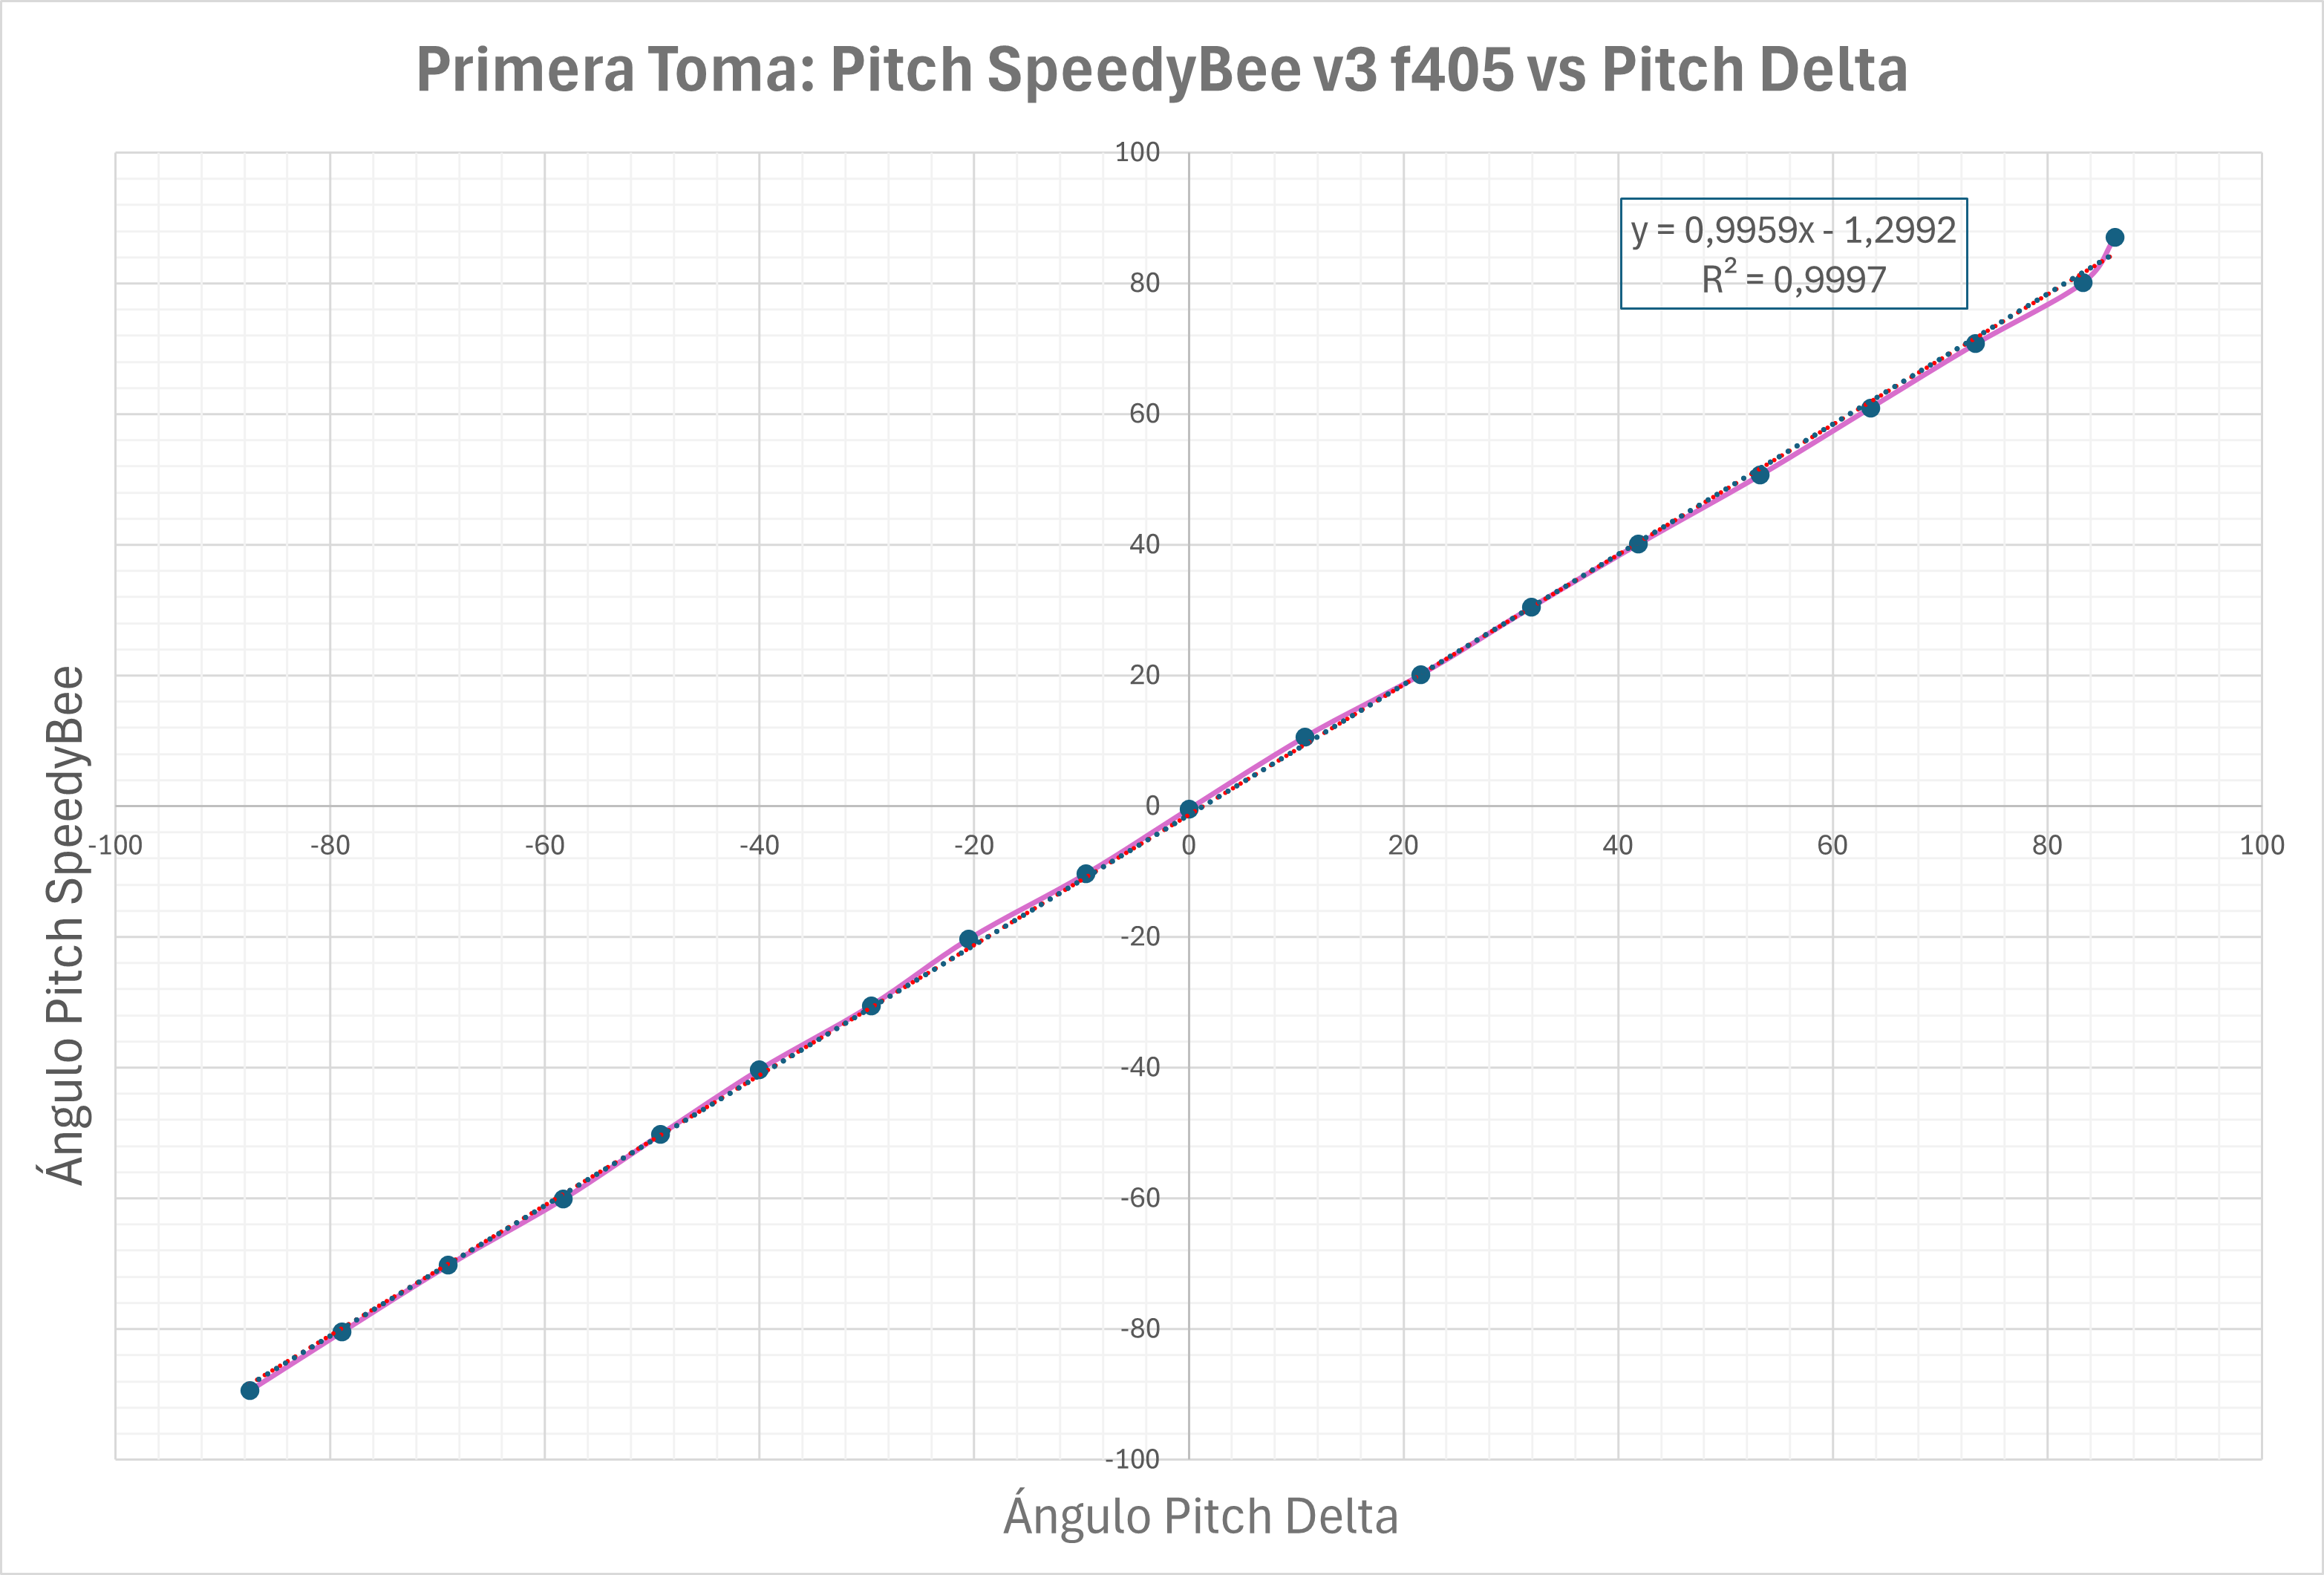
\includegraphics[width=5.5 in]{Imagenes/Pruebas/pitch_1_compare.png}
                \caption{Comparación de Pitch entre controladores Delta y SpeedyBee V3 F405 en la primera toma de datos }
                \label{fig:comparacionPitch1}
            \end{figure}

            \begin{figure}[H]
                \centering
                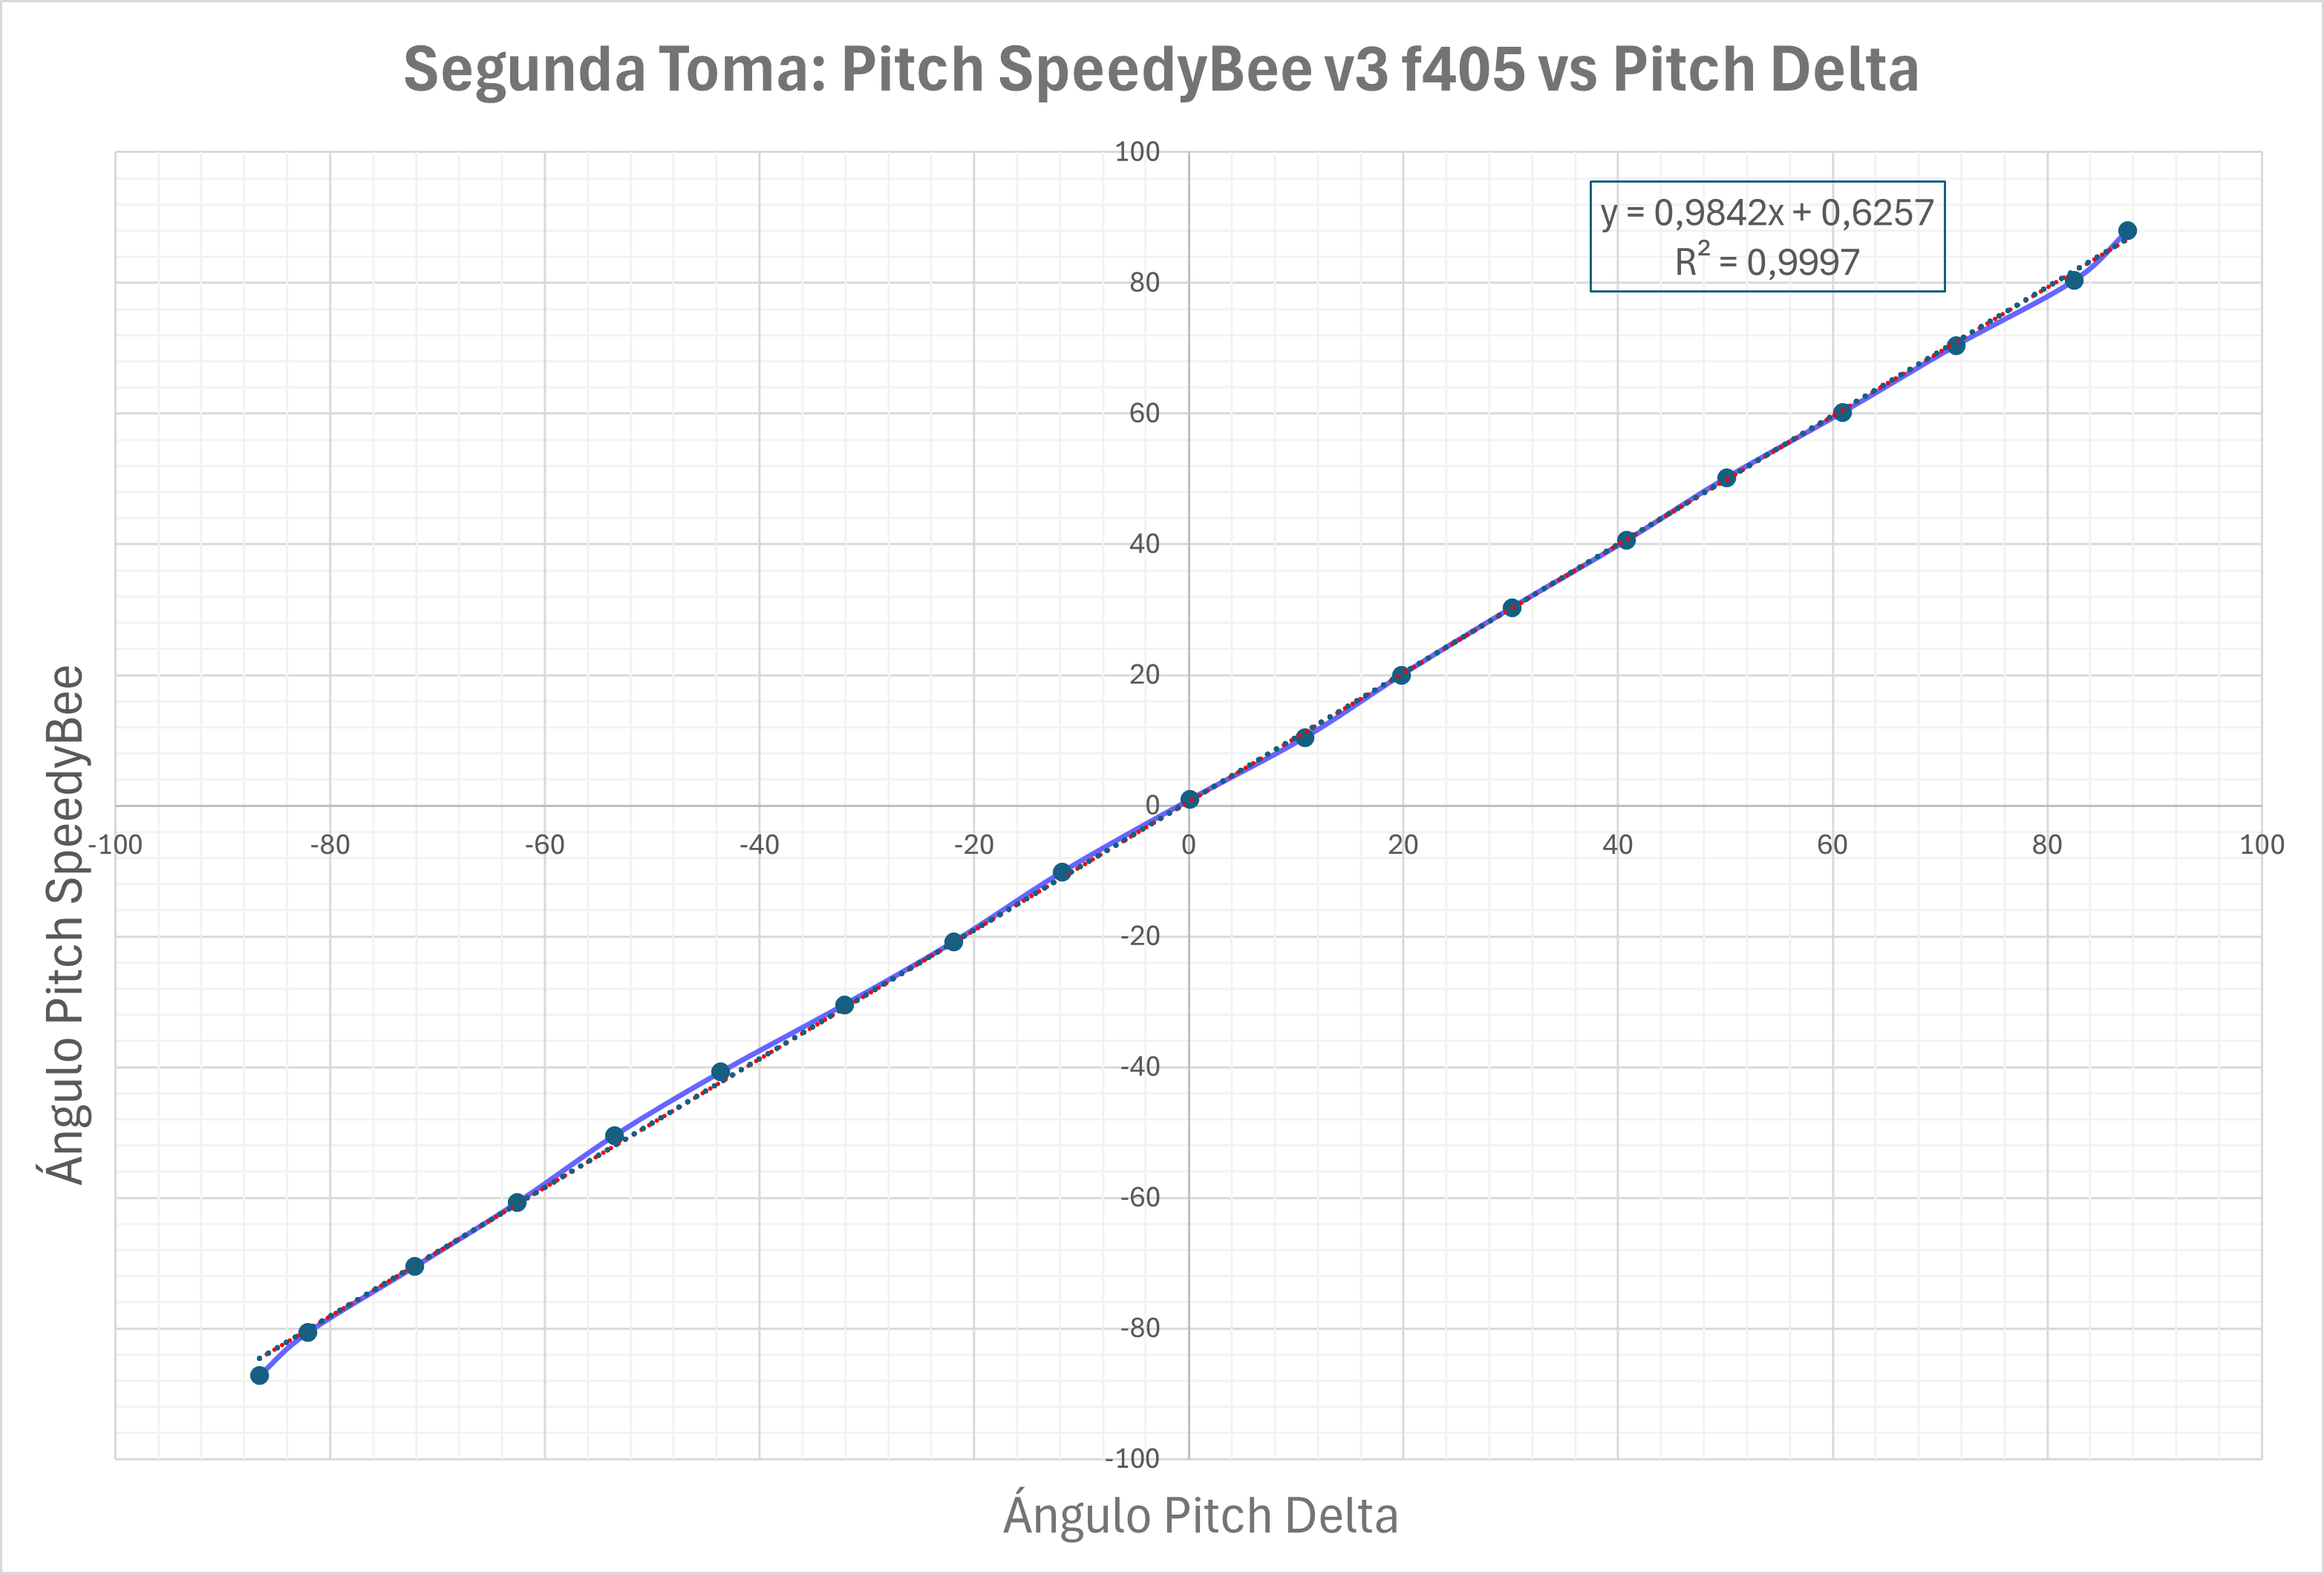
\includegraphics[width=5.5 in]{Imagenes/Pruebas/pitch_2_compare.png}
                \caption{Comparación de Roll entre controladores Delta y SpeedyBee V3 F405 en la segunda toma de datos }
                \label{fig:comparacionPitch2}
            \end{figure}


    \subsection{Pruebas de Variación de Altura con el Barómetro BMP280}

        Para evaluar el desempeño del sensor barométrico BMP280 en la medición de la altura, se realizó una prueba en el Edificio Mario Laserna. Durante esta prueba, se utilizó un ascensor para cambiar de piso en diferentes niveles del edificio. La prueba se inició en el nivel S2 y se ascendió hasta el piso 8. Finalmente, se descendió al nivel inicial y se capturaron los datos correspondientes a la variación de altura.

        \subsubsection{Procedimiento de la Prueba}

            \begin{enumerate}
                \item \textbf{Inicio en el Nivel S2}: La prueba comenzó en el nivel subterráneo 2 del edificio.
                \item \textbf{Ascenso al Piso 8}: Se utilizó el ascensor para ascender secuencialmente desde el nivel S2 hasta el piso 8, realizando paradas en cada piso para registrar los datos de altura.
                \item \textbf{Descenso al Nivel Inicial}: Posteriormente, se descendió de nuevo hasta el nivel S2, registrando los datos durante todo el recorrido.
            \end{enumerate}

        \subsubsection{Resultados}

            La figura adjunta muestra los resultados obtenidos de la prueba de variación de altura. Se puede observar cómo la altura medida por el BMP280 cambia a medida que el sensor se mueve a diferentes niveles del edificio. Los datos capturados reflejan un aumento progresivo de la altura durante el ascenso y una disminución correspondiente durante el descenso.

            \begin{figure}[H]
                \centering
                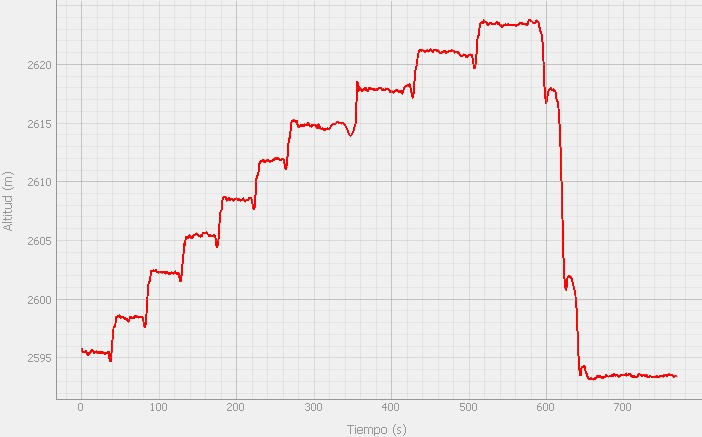
\includegraphics[width=0.8\textwidth]{Imagenes/Pruebas/altura.jpg}
                \caption{Variación de altura medida por el BMP280 durante el ascenso y descenso en el Edificio Mario Laserna.}
                \label{fig:variacion_altura}
            \end{figure}

        \subsubsection{Análisis de las Alturas del Edificio}

            La prueba de variación de altura realizada en el Edificio Mario Laserna nos permitió obtener datos precisos sobre la altitud a diferentes niveles del edificio. Según los datos registrados, la altura en el nivel S2 era de aproximadamente 2595 metros sobre el nivel del mar (msnm), mientras que en el piso 8 la altura era de aproximadamente 2625 metros msnm.

            Para calcular la diferencia de altura entre estos dos niveles, se realiza la siguiente operación:

            \[
            \text{Diferencia de altura} = 2625 \, \text{msnm} - 2595 \, \text{msnm} = 30 \, \text{metros}
            \]

            Por lo tanto, la altura total del edificio, desde el nivel S2 hasta el piso 8, es de 30 metros.

            Estos resultados demuestran la capacidad del sensor BMP280 para medir con precisión las variaciones de altura en un entorno controlado como el de un edificio de varios pisos.



    \subsection{Pruebas de GPS}
        Se realizó una prueba de GPS en el espacio abierto conocido como \textbf{El Bobo} en la Universidad de los Andes. Durante esta prueba, los datos de ubicación fueron almacenados en la tarjeta SD del dispositivo para su posterior análisis y ploteo en un mapa. Tal y como se muestra en la imagen adjunta, se realizó un desplazamiento en forma de bucle para verificar la precisión del GPS.

        El recorrido se realizó alrededor de la zona verde, registrando puntos de ubicación en intervalos regulares. Los datos capturados fueron luego representados en un mapa, mostrando el trayecto seguido. Esta prueba permitió evaluar la precisión del GPS en un entorno controlado y abierto, confirmando su capacidad para rastrear movimientos en tiempo real y proporcionar datos de ubicación precisos.

        \begin{figure}[H]
        \centering
        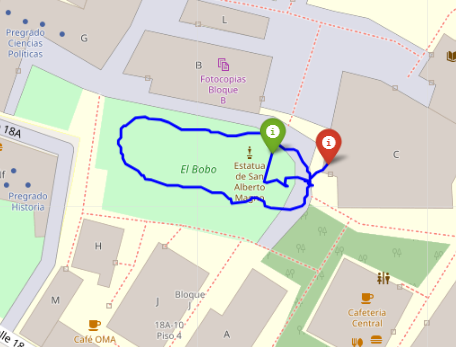
\includegraphics[width=0.8\textwidth]{Imagenes/Pruebas/gps.png}
        \caption{Recorrido de prueba de GPS en \textbf{El Bobo}, Universidad de los Andes.}
        \label{fig
        }
        \end{figure}
\clearpage
%\input{Sections/vuelo}
\clearpage
%
\section{Prueba de vuelo}

    Se realizó una prueba de vuelo para comprobar el funcionamiento del controlador Delta 2.0 en un UAV de ala fija. Esta prueba se realizó en la Pista de Aeromodelismo Vuelo Libre, en Tenjo, Cundinamarca, Colombia. 

    El controlador de vuelo fue instalado en el fuselaje de un avión tipo Protégé de Carl Goldberg, justo debajo de las alas. Esta ubicación estratégica permite un fácil acceso y brinda la protección adecuada para los componentes electrónicos durante el vuelo. (veasé \ref{fig:protege})

    \begin{itemize}
        \item \textbf{Imagen Izquierda:} La imagen muestra la instalación del controlador de vuelo dentro del fuselaje del avión. Se puede ver que el controlador está firmemente sujeto justo debajo de las alas. Esta posición facilita la conexión con otros componentes del sistema de vuelo y asegura que el controlador permanezca estable durante el vuelo.
        
        \item \textbf{Imagen Derecha:} La imagen muestra el UAV-RAS Uniandes tipo Protégé completamente ensamblado y listo para volar. Se puede apreciar cómo el controlador de vuelo está integrado de manera discreta en el fuselaje, sin interferir con la aerodinámica del avión.
    \end{itemize}


    \begin{figure}[H]
        \centering
        \includegraphics[width=\textwidth]{Imagenes/Pruebas/UAV protegé.png}
        \caption{Instalación del Controlador de Vuelo Protégé}
        \label{fig:protege}
    \end{figure}


    \subsection{Metodología de la Prueba}

        En esta prueba se tiene una comunicación bidireccional entre la tarjeta en base y la tarjeta en vuelo. La tarjeta en base es conectada mediante un cable tipo C de transmisión de datos a un ordenador que despliega la interfaz, tal como se muestra en la figura \ref{fig:diagrama_prueba_vuelo}.

        Las pruebas que se llevaron a cabo se dividen en cinco categorías principales: Sensórica, Actuadores, GPS, Comunicación, Almacenamiento de Datos e Interfaz. Las pruebas se llevaron a cabo en tres fases: en tierra, durante el montaje en el UAV y en vuelo.\\


        En la categoría de sensórica, las lecturas del giroscopio (Yaw, Pitch y Roll) fueron precisas en todas las fases, obteniendo una calificación del 100\%. Sin embargo, en las pruebas del barómetro se presentaron picos abruptos en las lecturas de presión atmosférica y altura durante el vuelo, lo que no fue consistente con la información de vuelo. Estos cambios abruptos en la recepción de datos resultaron en una calificación del 50\%.\\

        En cuanto a los actuadores, estos funcionaron perfectamente al usar el receptor FlySky. Estos mostraron un funcionamiento óptimo tanto en tierra como en vuelo, obteniendo una calificación del 100\%. Durante las pruebas en el montaje del UAV se presentaron delays en las señales del controlador y los servos, lo que resultaría en una afectación en las dinámicas del UAV. Por otro lado, debido a condiciones climáticas no se pudo realizar una prueba de vuelo con el controlador Delta 2.0 por lo que durante el vuelo con el FlySky se posicionó el controlador de vuelo en el interior del UAV pero sin conectar los servos del UAV a este.\\

        En la categoría de GPS, la calibración y recepción de datos fueron correctas en tierra y durante el montaje en el UAV. Sin embargo, durante el vuelo, el tiempo de actualización del GPS no fue lo suficientemente rápido, lo que llevó a pérdidas de conexión con el satélite y resultó en una calificación del 70\%. Este problema causó saltos abruptos en la localización del UAV.\\

        La Comunicación bidireccional entre la estación en tierra y el UAV fue efectiva en tierra, pero durante el vuelo se presentaron corrupciones de paquetes que afectaron la transmisión y recepción de datos. Esto resultó en calificaciones del 85\% y 30\% para la transmisión de datos del giroscopio y el barómetro, respectivamente. Además, hubo una gran pérdida de datos respecto a los datos transmitidos por la tarjeta en vuelo.\\

        En la categoría de Almacenamiento de Datos, tanto la estación en tierra como el controlador de vuelo fueron capaces de almacenar datos correctamente en tierra. Sin embargo, durante el vuelo, hubo pérdidas ocasionales de datos, resultando en una calificación del 70\% para el controlador de vuelo. Este problema fue causado por la frecuencia de datos transmitidos y la capacidad de almacenamiento del sistema.\\

        Finalmente, en la categoría de Interfaz, el despliegue y la visualización de datos fueron correctos en tierra. Sin embargo, durante el vuelo, se observaron delays y corrupción de datos en la tarjeta de vuelo, resultando en una calificación del 50\%. La tarjeta de la estación en tierra funcionó adecuadamente, pero la tarjeta de vuelo mostró problemas significativos.\\
        \begin{figure}[H]
            \centering
            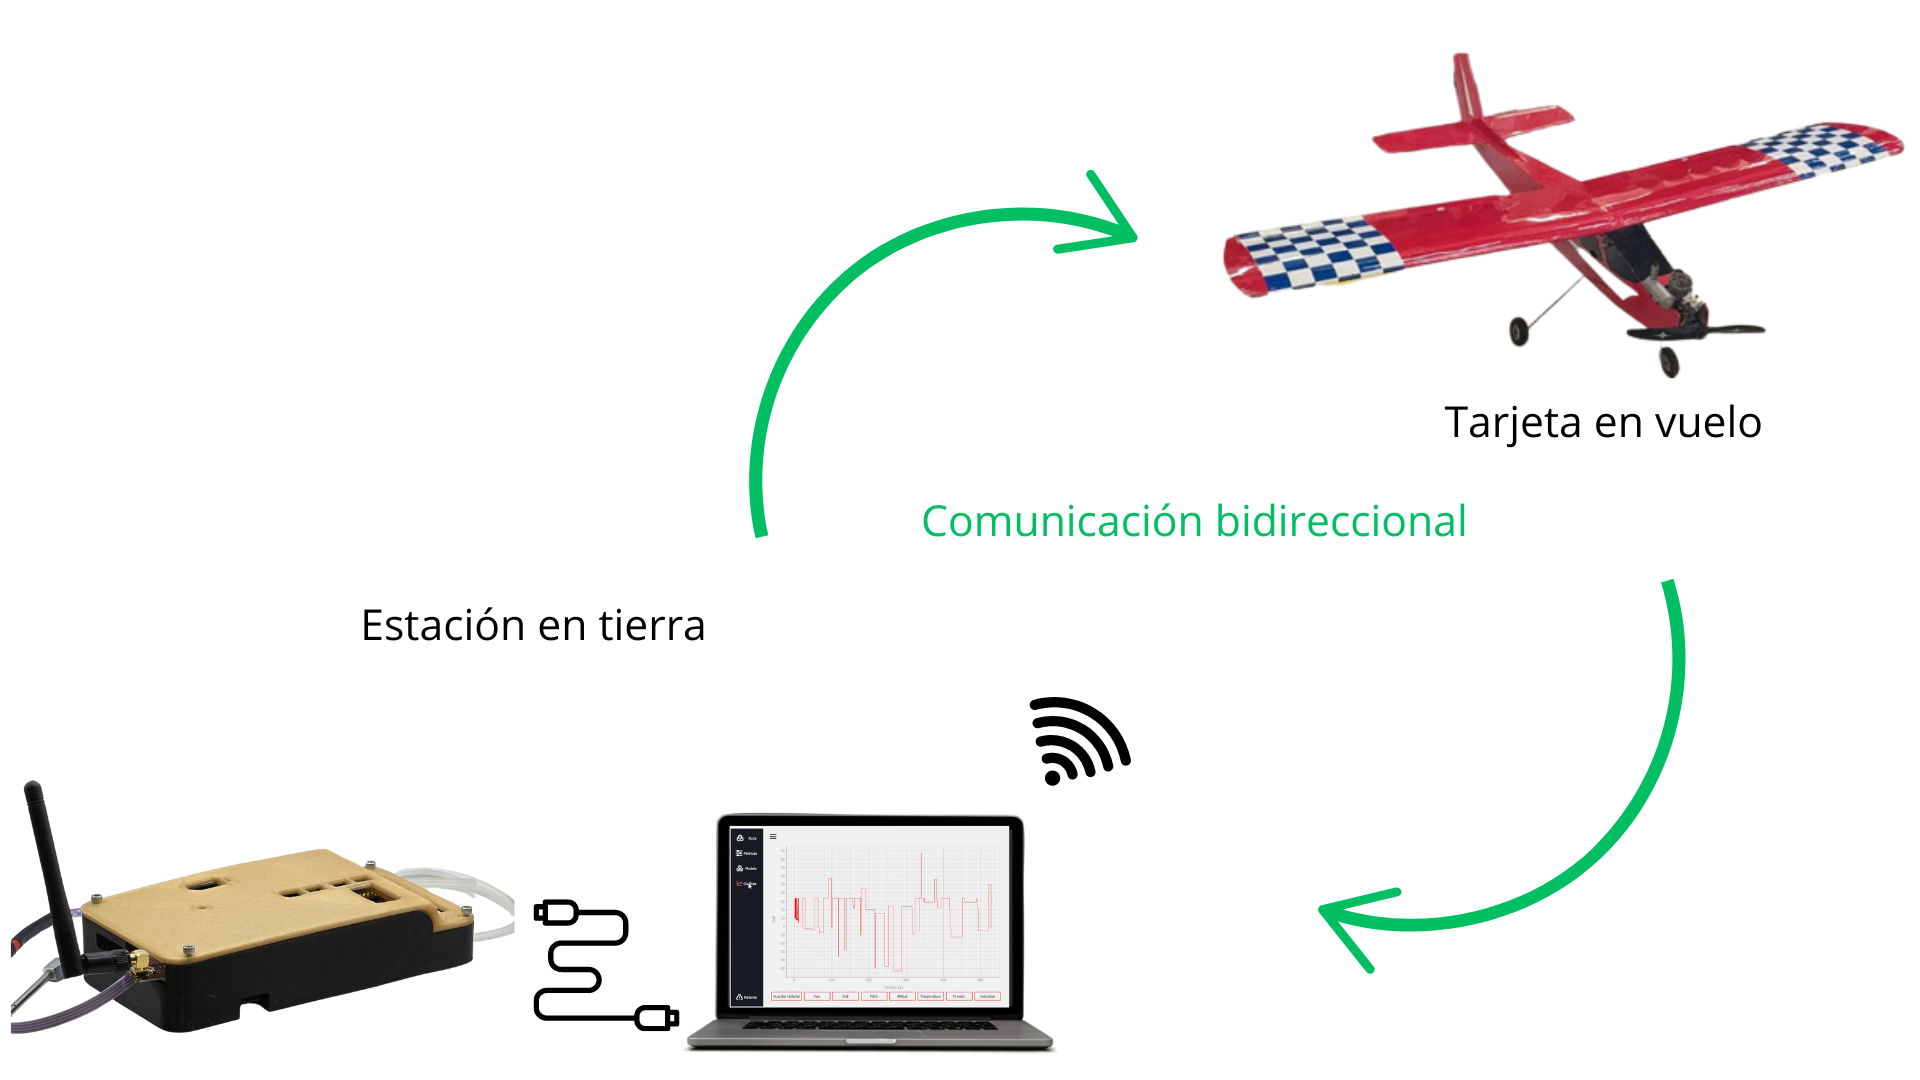
\includegraphics[width=12  cm]{Imagenes/Pruebas/Esquematico.png}
            \caption{Diagrama de la prueba de vuelo}
            \label{fig:diagrama_prueba_vuelo}
        \end{figure}


    \clearpage
    \subsection{Matriz de Rendimiento de la Prueba de vuelo}
        A continuación se muestra la matriz de rendimiento de la prueba de vuelo\ref{fig:matriz_prueba_vuelo}:

        \begin{figure}[H]
            \centering
            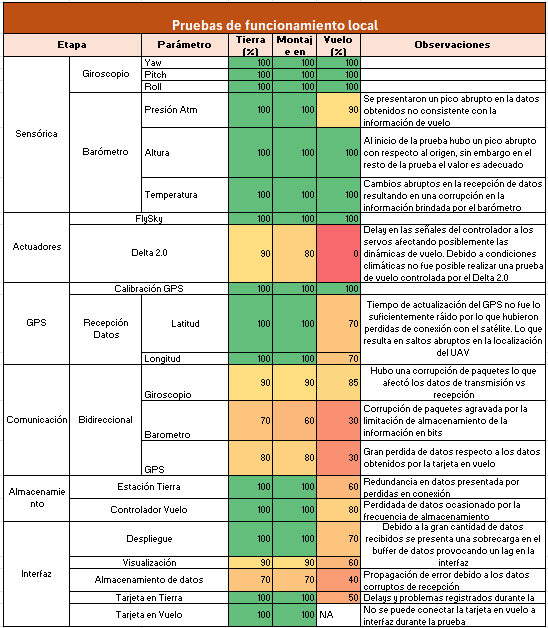
\includegraphics[width=\textwidth]{Imagenes/Pruebas/matriz_prueba_vuelo_local.png}
            \caption{Matriz de evaluación para prueba de vuelo}
            \label{fig:matriz_prueba_vuelo}
        \end{figure}

        El desempeño general de las pruebas evidencia un comportamiento sólido en tierra y durante el montaje en el UAV. Por otro lado, se evidencian algunas dificultades notables durante las pruebas de vuelo, especialmente en las áreas de comunicación bidireccional, almacenamiento de datos y la interfaz de usuario. Estas áreas requieren una revisión y optimización para asegurar un rendimiento óptimo en condiciones de vuelo.

        A continuación se muestra el rendimiento general de la prueba de vuelo\ref{fig:resumen_prueba_vuelo}:

        \begin{figure}[H]
            \centering
            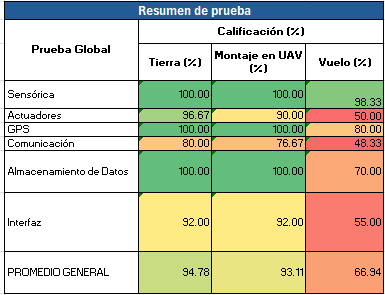
\includegraphics[width=10cm]{Imagenes/Pruebas/resumen_prueba_vuelo_local.png}
            \caption{Matriz de evaluación para prueba de vuelo}
            \label{fig:resumen_prueba_vuelo}
        \end{figure}
\clearpage
%\section{Resultados Prueba de Vuelo}
    \subsection{Análisis de Resultados GPS Controlador de Vuelo}

        A continuación, se presenta los resultados obtenidos de la trayectoría GPS del UAV de ala fija. La figura \ref{fig:GPS_pruebaVuelo} muestra el recorrido efectuado por el UAV de ala fija durante la prueba de vuelo, la cual fue realizada por un piloto especializado especializado en el manejo de este tipo de aeronaves. La trayectoria registrada refleja la complejidad del vuelo, donde el piloto ejecutó diversas maniobras y movimientos a lo largo de un periodo prolongado. La capacidad del piloto para controlar el UAV se evidencia en las variaciones y cambios de dirección observados en la imagen. Se resalta el hecho de que en esta imagen no se puede observar adecuadamente como fue el recorrido de la aeronave, ya que hay gran variedad de virajes realizadas por la aeronave. 
        \begin{figure}[H]
            \centering
            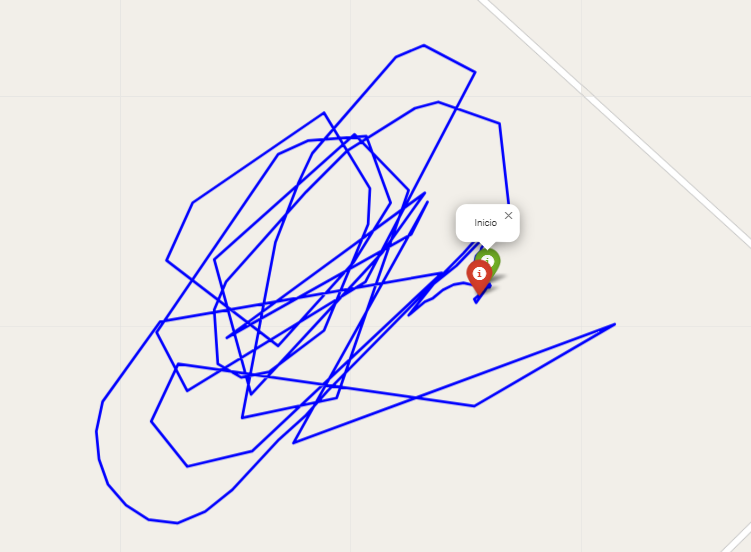
\includegraphics[width=12 cm]{Imagenes/Vuelo/gps_Prueba.png}
            \caption{Recorrido del UAV prueba de Vuelo}
            \label{fig:GPS_pruebaVuelo}
        \end{figure}

        Seguidamente se realizo una imagen que proporciona una visualización en 3D del movimiento del UAV en relación con su altitud (véase \ref{fig:GPS_altitud}). En esta gráfica, se distinguen claramente las fases de ascenso y descenso del UAV, con diferentes colores para cada fase del vuelo: \\

        Ascenso (Azul): La sección marcada en azul muestra el trayecto de ascenso del UAV. Se observa una subida gradual y controlada en la altitud, lo que indica que el piloto pudo manejar eficientemente el aumento de altitud del UAV.\\
        Descenso (Verde): La sección marcada en verde indica el trayecto de descenso. Al igual que en el ascenso, el descenso muestra una disminución gradual y controlada en la altitud, lo que sugiere un buen desempeño del piloto en la fase de descenso.


        \begin{figure}[H]
            \centering
            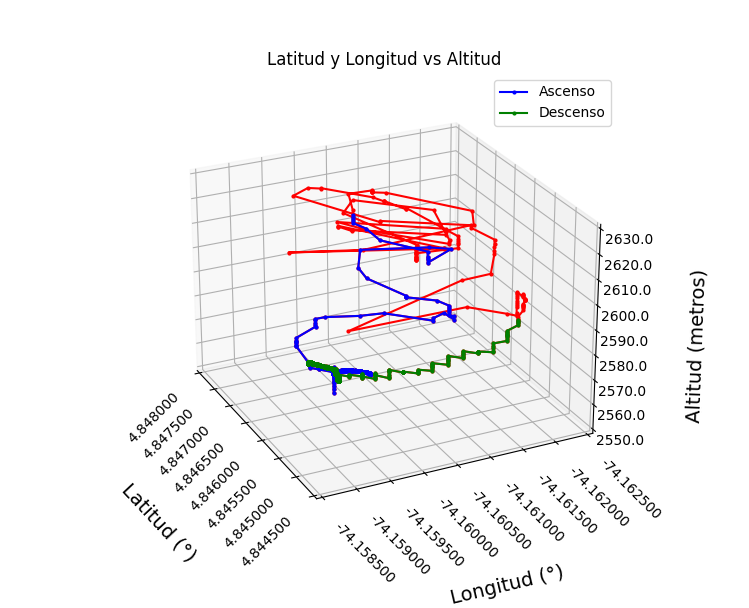
\includegraphics[width=\textwidth]{Imagenes/Vuelo/latitud y longitud acenso.png}
            \caption{Latitud y Longitud vs Altitud}
            \label{fig:GPS_altitud}
        \end{figure}


    \subsection{Datos Recibidos del Barómetro BMP280 Controlador de Vuelo}
        Los datos obtenidos del barómetro BMP280 durante la prueba de vuelo del UAV se pueden observar a continuación (véase \ref{fig:datos obtenidos bmp280}). En donde podemos contrastar altitud, temperatura y presión vs tiempo.\\
        \begin{itemize}
            \item \textbf{Altitud vs Tiempo:} Entre aproximadamente 600 y 1150 segundos se realizó la prueba de vuelo, observándose un aumento de altitud de alrededor de 60 metros. A los 1100 segundos se aprecia una bajada progresiva de nivel, que corresponde a las maniobras de descenso del UAV.\\
            \item \textbf{Temperatura vs Tiempo:} La temperatura medida dentro del dispositivo muestra un aumento progresivo durante el periodo de vuelo, reflejando el calentamiento de los componentes internos del UAV.\\
            \item \textbf{Presión vs Tiempo:} La presión atmosférica se mantuvo estable la mayor parte del tiempo, excepto durante el ascenso del UAV, donde se registró una caída significativa, lo que es coherente con el aumento de altitud. Posteriormente, la presión se estabiliza una vez que el UAV alcanza su altitud máxima y durante el descenso.
            
        \end{itemize}



        \begin{figure}[H]
            \centering
            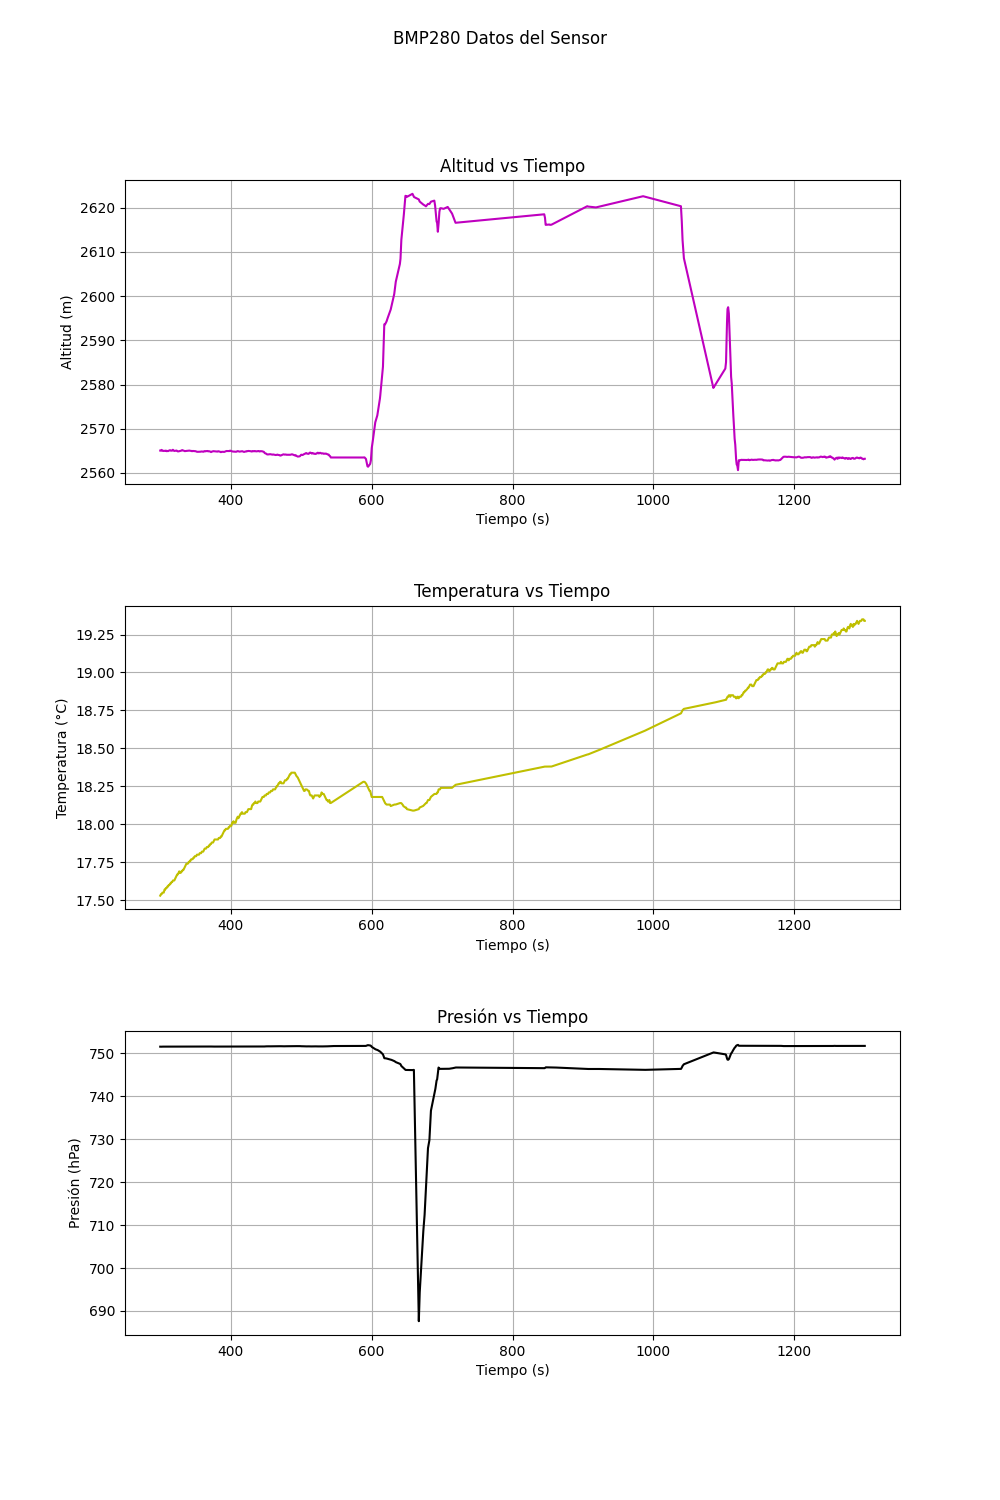
\includegraphics[width=\textwidth]{Imagenes/Vuelo/BMP280_sensor.png}
            \caption{Datos Obtenidos BMP280}
            \label{fig:datos obtenidos bmp280}
        \end{figure}



        En resumen, los datos indican que el vuelo realizado por el piloto fue exitoso. El incremento en altitud, el comportamiento térmico y las variaciones en la presión atmosférica observadas son coherentes con las expectativas de un vuelo controlado. 


    \subsection{Análisis de Resultados de los Ángulos de Movimiento del UAV Controlador de Vuelo}
        Datos Recibidos del Sensor BNO055
        Los datos de orientación obtenidos del sensor BNO055 durante la prueba de vuelo del UAV.  En las figuras  \ref{fig:datosYawPitch, roll} y \ref{fig:datos obtenidos BNO055} se pueden observar los registros de los ángulos de roll, pitch, yaw y compass a lo largo del tiempo. Estos gráficos muestran cómo el UAV se comportó en términos de orientación durante las diferentes fases del vuelo. \\ 

        \begin{itemize}
            \item \textbf{Roll vs Tiempo:} El ángulo de roll varía entre -40 y 80 grados. Estas variaciones son típicas en aeronaves, ya que valores cercanos a 90 grados podrían comprometer la estabilidad del UAV. Los valores observados son comunes en los ángulos de banqueo de la aeronave.\\

            \item \textbf{Pitch vs Tiempo:} El ángulo de pitch varía entre -40 y 40 grados. Estos valores son usuales para evitar que la aeronave entre en situaciones de "pique", lo que podría ser peligroso. Se mantuvo cuidado en esta parte para asegurar la estabilidad del UAV.\\

        \item \textbf{Yaw vs Tiempo: }El ángulo de yaw muestra oscilaciones características durante los virajes de la aeronave. Estos cambios abruptos en la orientación están relacionados con los giros efectuados por el piloto.\\

        \item \textbf{Compass vs Tiempo:}Similar al yaw, el compás muestra oscilaciones durante los virajes, reflejando los cambios de dirección del UAV. La coincidencia de estos cambios con el roll indica la correlación entre los virajes y el banqueo de la aeronave.
        \end{itemize}


        \begin{figure}[H]
            \centering
            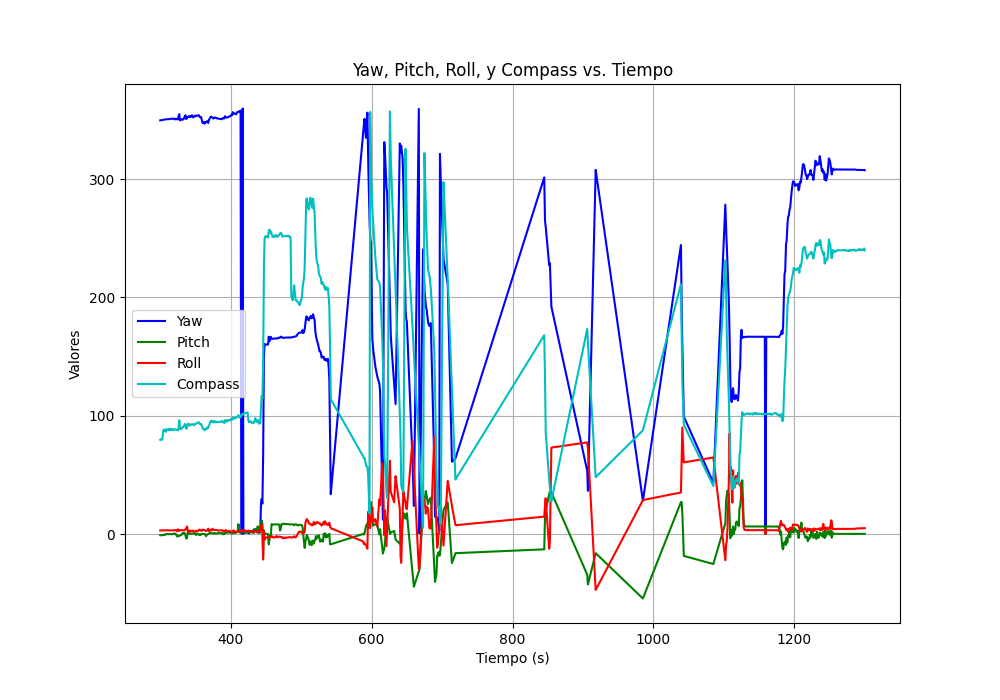
\includegraphics[width=13 cm]{Imagenes/Vuelo/yaw_pitch_roll_vs_tiempo.png}
            \caption{Yaw, Pitch, Roll y Compas vs Tiempo}
            \label{fig:datosYawPitch, roll}
        \end{figure}


        \begin{figure}[H]
            \centering
            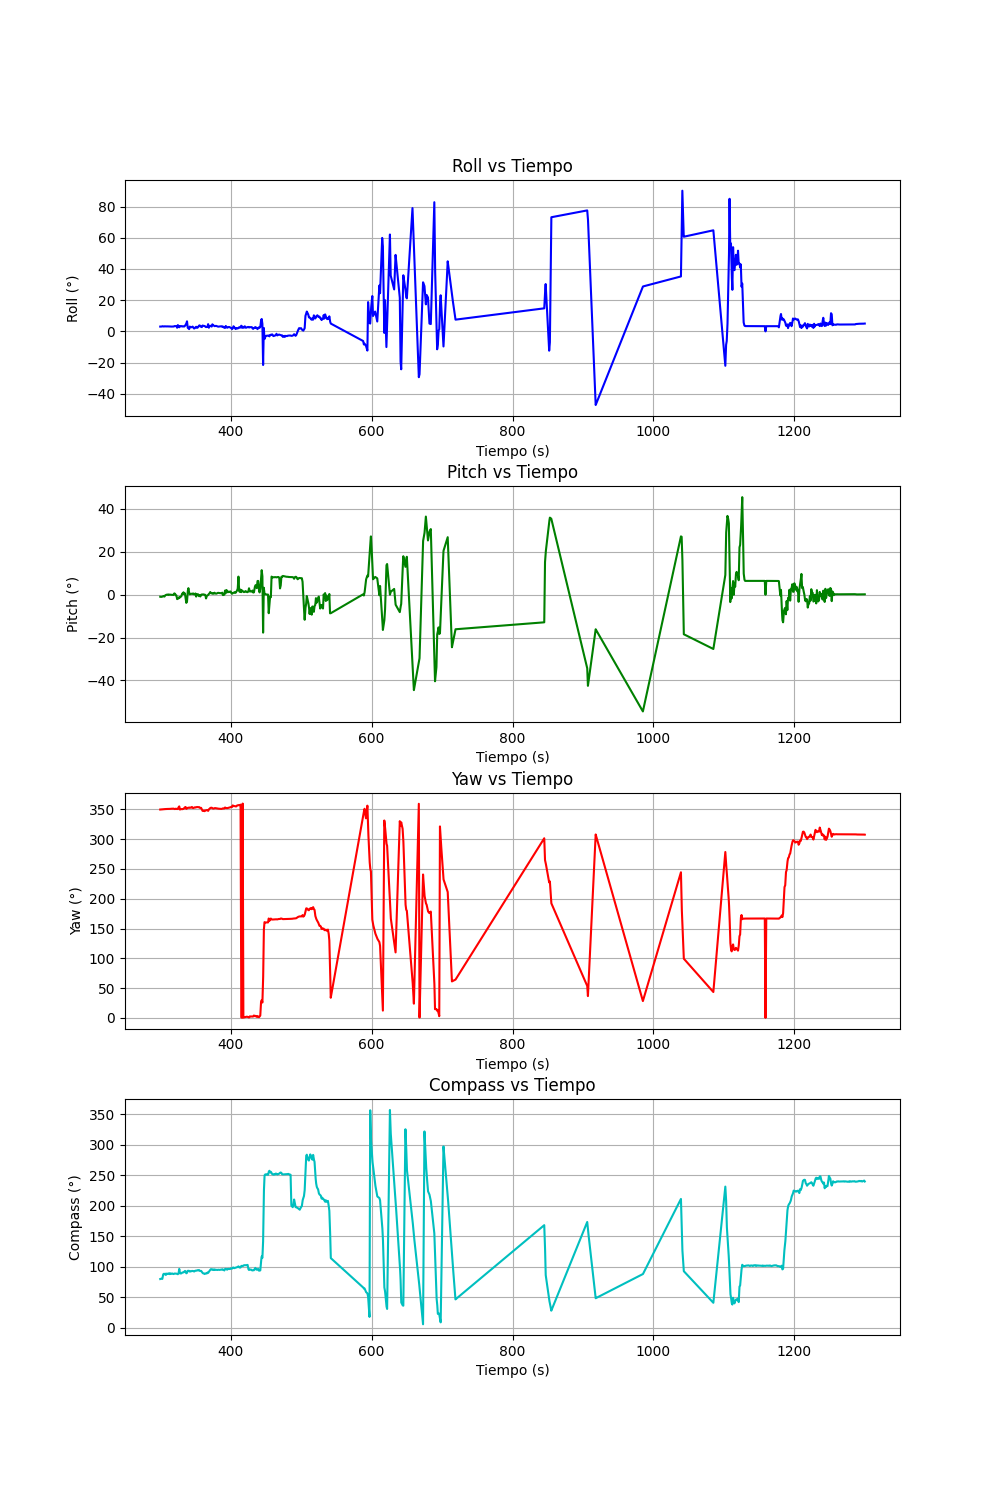
\includegraphics[width=15 cm]{Imagenes/Vuelo/BNO055_orientacion.png}
            \caption{Datos Obtenidos BNO055}
            \label{fig:datos obtenidos BNO055}
        \end{figure}


    \subsection{Transmisión y Recepción de Datos}

        La figura \ref{fig:comparacion transmision y recepcion} muestra los datos transmitidos y recibidos durante la experimentación del vuelo del UAV. Aunque en algunos momentos los datos parecen coincidir, hay varios puntos en los que se observa una considerable pérdida de paquetes y corrupción de datos.\\

        En el caso de la altitud, hay un gran desequilibrio entre los datos enviados y recibidos, con diferencias notables que indican transmisiones fallidas. Esto sugiere que hubo errores en la codificación de los datos antes de su transmisión y en la decodificación después de su recepción. Si estos procesos no se realizan correctamente, los datos pueden llegar dañados, justificando la discrepancia observada.\\

        Los datos de presión también muestran una gran diferencia entre los valores transmitidos y recibidos. Este problema podría deberse a la pérdida parcial de paquetes durante la transmisión. El módulo nRF24L01, limitado a 32 bits por paquete, puede experimentar pérdidas fraccionarias que afectan severamente la integridad de los datos. La pérdida o corrupción de partes de un paquete puede hacer que los datos recibidos sean muy diferentes de los datos transmitidos.\\

        Al observar los puntos obtenidos del GPS, se detecta una pérdida considerable de información transmitida durante el vuelo. Se observan incongruencias en los valores obtenidos, como 21.478790,529.000000, que no es una posición geográfica válida. Además, muchos valores del vuelo no se actualizaron correctamente, lo que sugiere una corrupción y pérdida sustancial de la información.\\

        Estas observaciones destacan la necesidad de revisar y mejorar los procesos de codificación y decodificación para asegurar que los datos se transmitan y reciban de manera precisa y coherente, minimizando las pérdidas y corrupciones en futuras pruebas de vuelo del UAV.



        \begin{figure}[H]
            \centering
            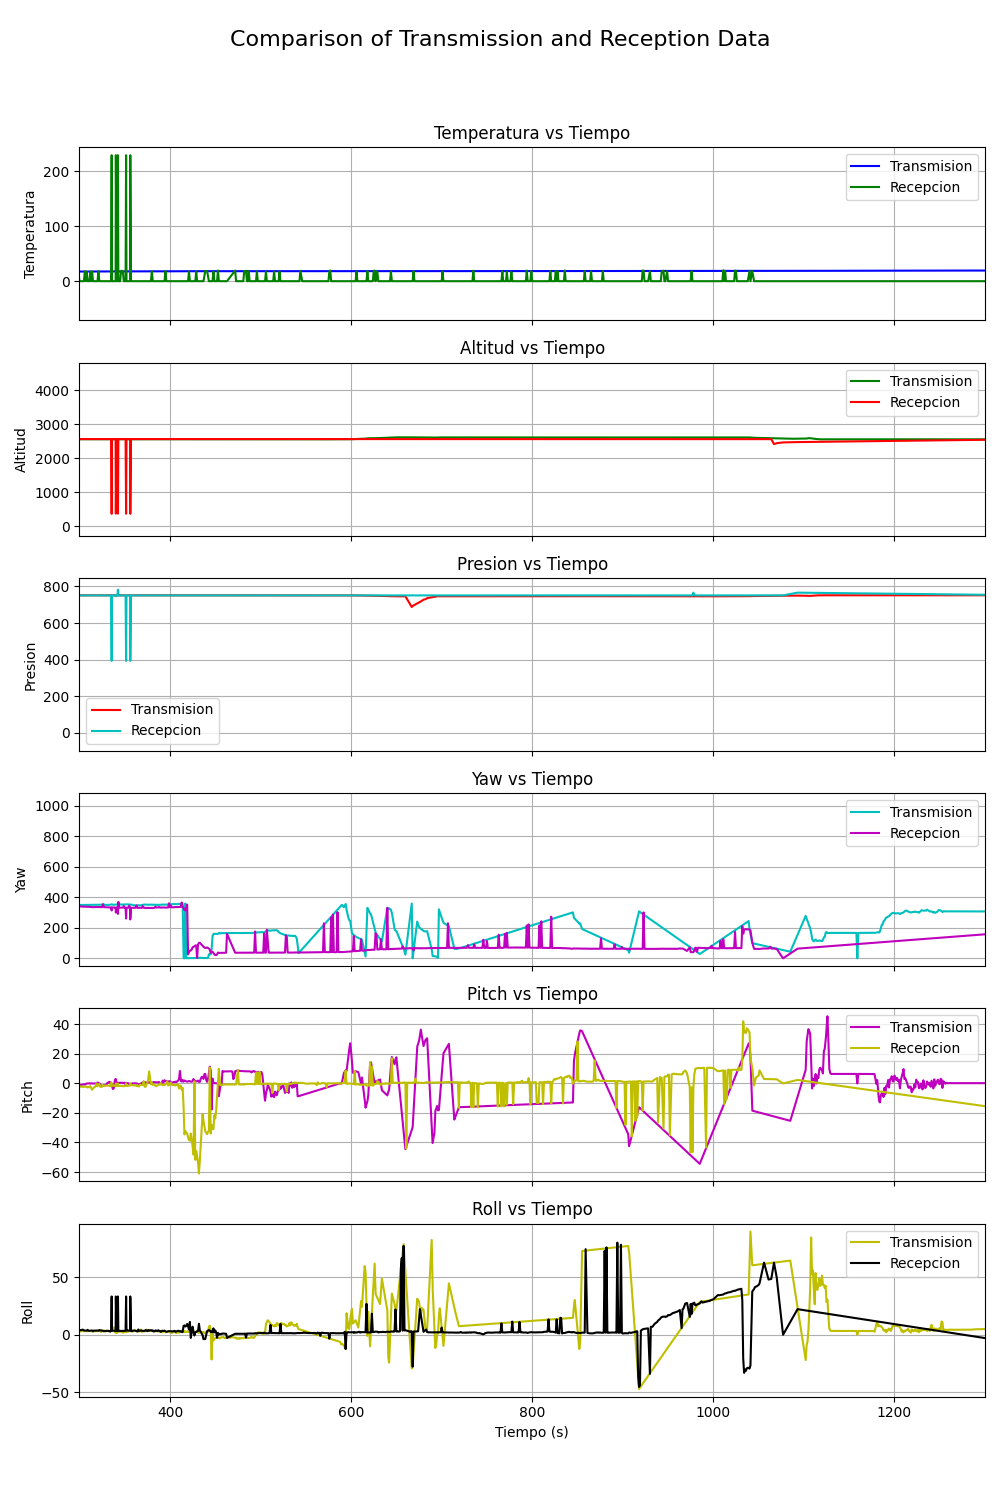
\includegraphics[width=\textwidth]{Imagenes/Vuelo/comparison_subplots.png}
            \caption{Comparación datos Transmisión y Recepción}
            \label{fig:comparacion transmision y recepcion}
        \end{figure}

    \subsection{Recepción datos de la Interfaz}


        La figura  \ref{fig:Datos guardados Interfaz} muestra los datos visualizados por la interfaz de comunicación durante el vuelo del UAV, mostrando al igual que como se hizo anteriormente las variables previamente expuestas. En este grafico, a diferencia de los anteriores se muestran picos y fluctuaciones de las distintas señales. Se hace notable que las señales son representadas con pulsos cuadrados, lo que indica problemas en la recepción de información. \\

        Los datos de altitud presentan numerosos picos, sugiriendo interrupciones y pérdidas de paquetes. Esto refleja problemas significativos en la transmisión de esta información. La temperatura muestra inconsistencias similares, con picos abruptos que indican que no se recibió adecuadamente la información. Los datos de presión también tienen grandes fluctuaciones, lo que sugiere problemas en la transmisión y recepción de esta variable. Además, las variables de orientación (yaw, pitch, roll) muestran variaciones bruscas y picos, reflejando inconsistencias y posibles pérdidas de datos durante la transmisión.

    \subsubsection{Problemas Identificados}
        La transmisión de datos está generando un cuello de botella que afecta la integridad de la información recibida. Esto se debe a la limitación del módulo nRF24L01, que puede experimentar pérdidas de paquetes y corrupción de datos.

    \subsubsection{Solución Propuesta}
        Para mitigar estos problemas, es esencial implementar un buffer en la interfaz de la comunicación serial. Este buffer almacenará temporalmente los datos antes de su transmisión, permitiendo una mejor gestión del flujo de información y asegurando una transmisión más eficiente. Además, es crucial optimizar la interfaz de usuario para evitar lags y asegurar una fluidez correcta en la visualización de los datos. Esto mejorará la capacidad de monitoreo en tiempo real y la fiabilidad de la información presentada.

    \begin{figure}[H]
        \centering
        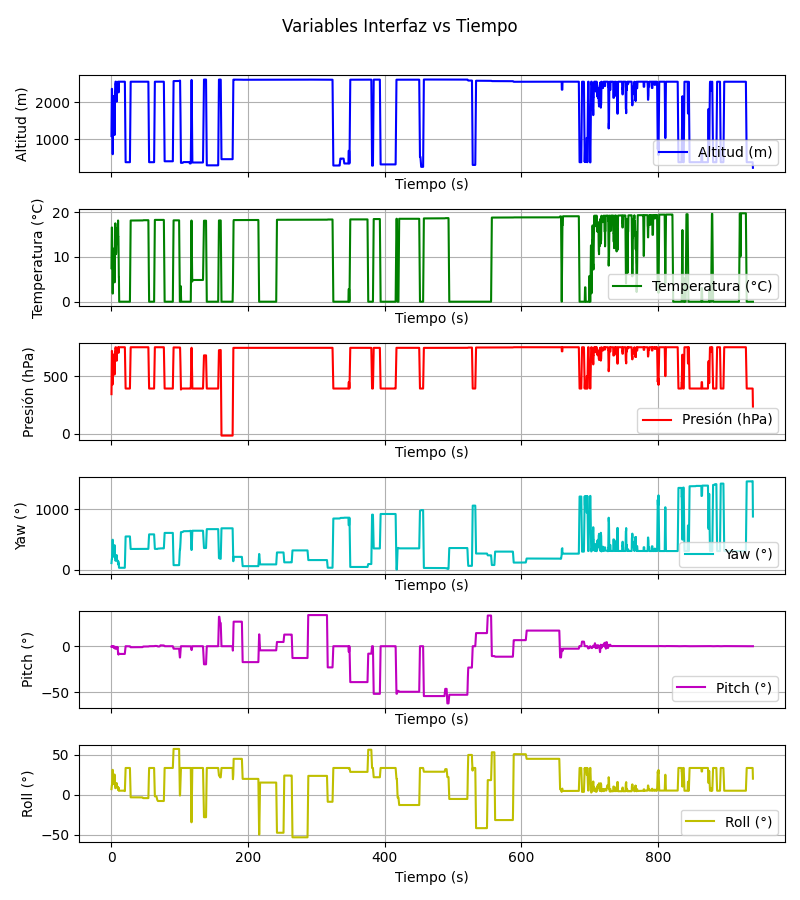
\includegraphics[width=\textwidth]{Imagenes/Vuelo/subplots_interfaz.png}
        \caption{Datos Guardados Interfaz}
        \label{fig:Datos guardados Interfaz}
    \end{figure}

\clearpage

\section{Conclusiones}



En este proyecto se logró hacer el diseño de un controlador de vuelo el cual cumple con todos los requisitos para ser implementado en la operación de un UAV de ala fija. Este diseño se logró implementar y operar en una aeronave real. Esto mediante la conexión exitosa de sensores y actuadores con el controlador de vuelo.\\

Además, se hizo un diseño del firmware e interfaces de vuelo el cual incluye algoritmos de control y sistemas de comunicación con los sensores. Se lograron transmitir los datos de orientación, altura, presión atmosférica y temperatura a una estación en tierra donde se pudo visualizar y recuperar dicha información.\\

Adicionalmente, se verificó el funcionamiento de los distintos sensores integrados en la aeronave contribuyendo esto al diseño de un sistema expansible y modular, lo cual facilita futuras mejoras y la integración de nuevos componentes. Fue posible diseñar e implementar un controlador de vuelo que opera efectivamente en condiciones reales de vuelo. Transmitiendo datos de GPS y telemetría en tiempo real se logró correctamente, permitiendo una supervisión constante y la capacidad de analizar estos parámetros en tiempo real mediante el uso de una interfaz.\\



\section{Trabajos Futuros}

Durante el desarrollo del proyecto se evidenciaron los siguientes problemas:
\begin{itemize}
    \item \textbf{Pérdida y Corrupción de Datos:} Durante las pruebas de vuelo, se observó una considerable pérdida y corrupción de datos, especialmente en las variables de altitud y presión. Esta situación se debe a errores en la codificación y decodificación de los datos, así como a limitaciones en la capacidad de transmisión del módulo nRF24L01, que puede manejar solo hasta 32 bits por paquete.
    
    \item \textbf{Cuello de Botella en la Transmisión de Datos:} La transmisión de datos generó un cuello de botella, afectando la integridad de la información recibida. Para mitigar este problema, se propone implementar un buffer en la interfaz de la comunicación serial. Este buffer ayudará a gestionar mejor el flujo de datos, asegurando una transmisión más eficiente.
    
    \item \textbf{Optimización de la Interfaz de Usuario:} Es esencial optimizar la interfaz de usuario para evitar retrasos y asegurar una visualización más fluida de los datos. Esto mejorará la capacidad de monitoreo en tiempo real y la fiabilidad de la información presentada.

\end{itemize}


Los tres objetivos principales de mejora que se pueden seguir para hacer del sistema de control de vuelo de mejor calidad, más confiable y fuerte incluyen:\\

Primero, mejorar el hardware del proyecto al fusionar todos los módulos en una misma placa de circuito impreso, mejorando la eficiencia del dispositivo, reduciendo el ruido y mejorando la conectividad de un módulo a otro. La estabilidad del sistema eléctrico también mejorará con un segundo inversor y un regulador de potencia continuo. Además, un módulo adicional de protección contra el flujo de corriente inversa y un sistema de gestión de baterías (BMS) deben ser parte del sistema para proteger la batería del UAV, lo cual hará que el sistema en su conjunto sea aún más confiable y duradero.\\

En segundo lugar, se debe seleccionar un módulo de comunicación que tenga más capacidad de transmisión de bits, con  una mayor frecuencia de transmisión. Esto mejorará el flujo de datos con menos posibilidades de perdidas. También, con el uso de un sistema de comunicación, como MAVLink, se permitiría detectar fallas en la transmisión de paquetes y tener una fiabilidad mejorada en términos de transmisión de datos.\\

Finalmente, la interfaz de usuario debería ser mejorada y optimizada. La configuración de un buffer en la interfaz de comunicación serial hará que los datos entrantes se presenten correctamente de manera eficaz, mejorando la interfaz del usuario. 

Estas innovaciones permitirán al controlador de vuelo ser más robusto y estable, mejorando la eficiencia, estabilidad y seguridad del sistema, así como la calidad de la interacción con el usuario.

\section{Anexos}

\begin{figure}[H]
    \centering
    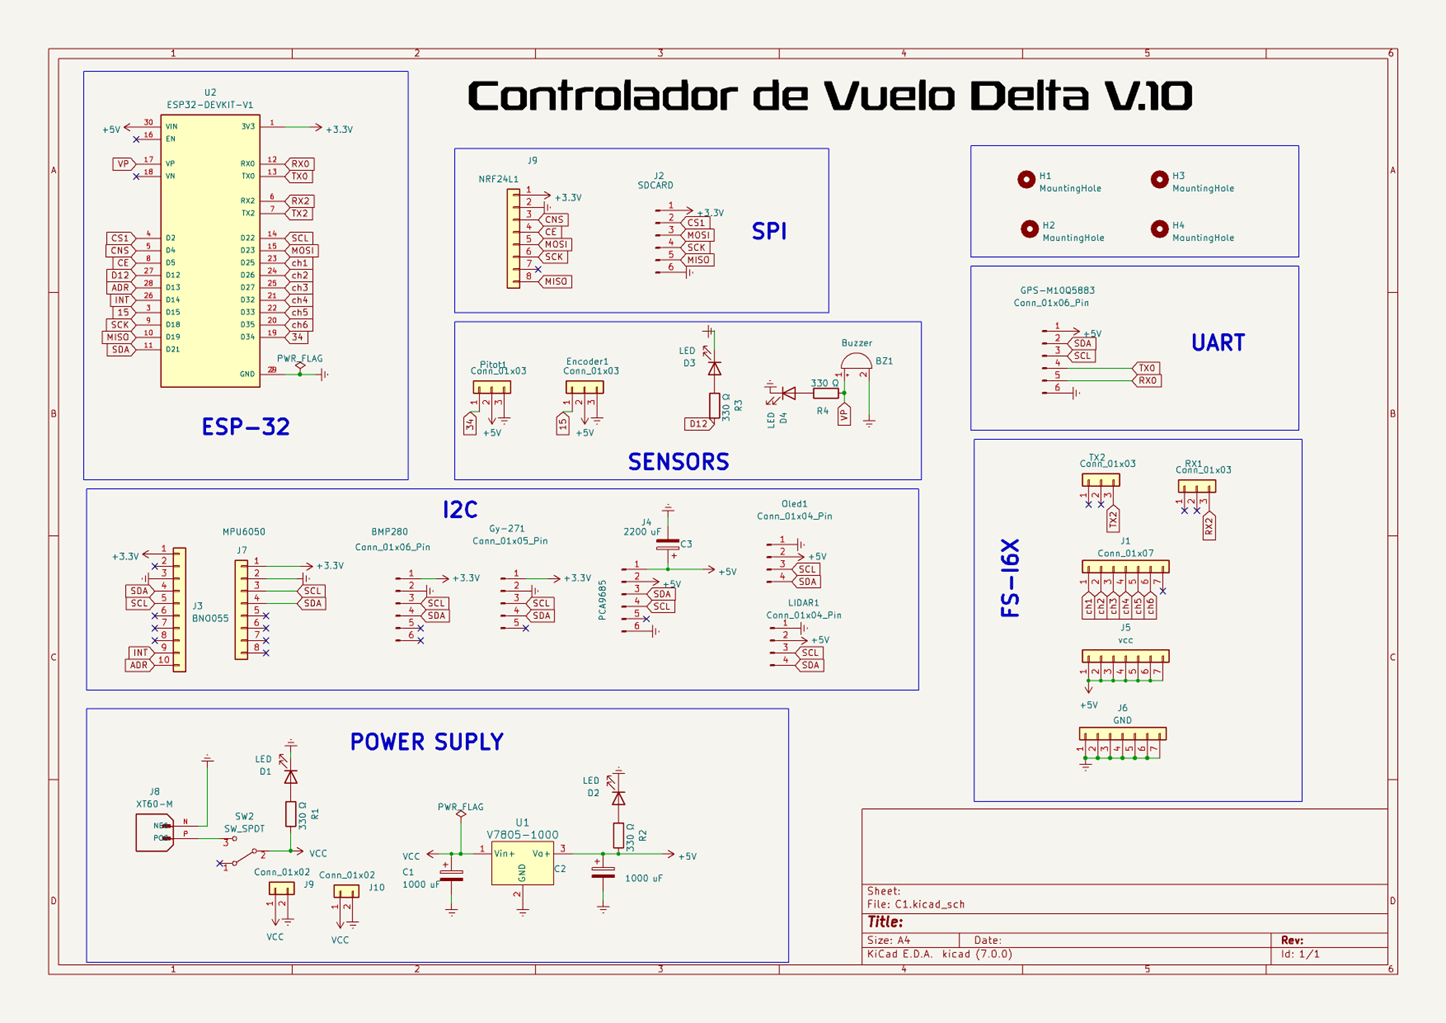
\includegraphics[width=\textwidth]{Imagenes/Anexos/esquematico_controlador_v1.png}
    \caption{Esquemático Circuito Impreso 1.0 }
    \label{fig:sch-1.0}
\end{figure}

\begin{figure}[H]
    \centering
    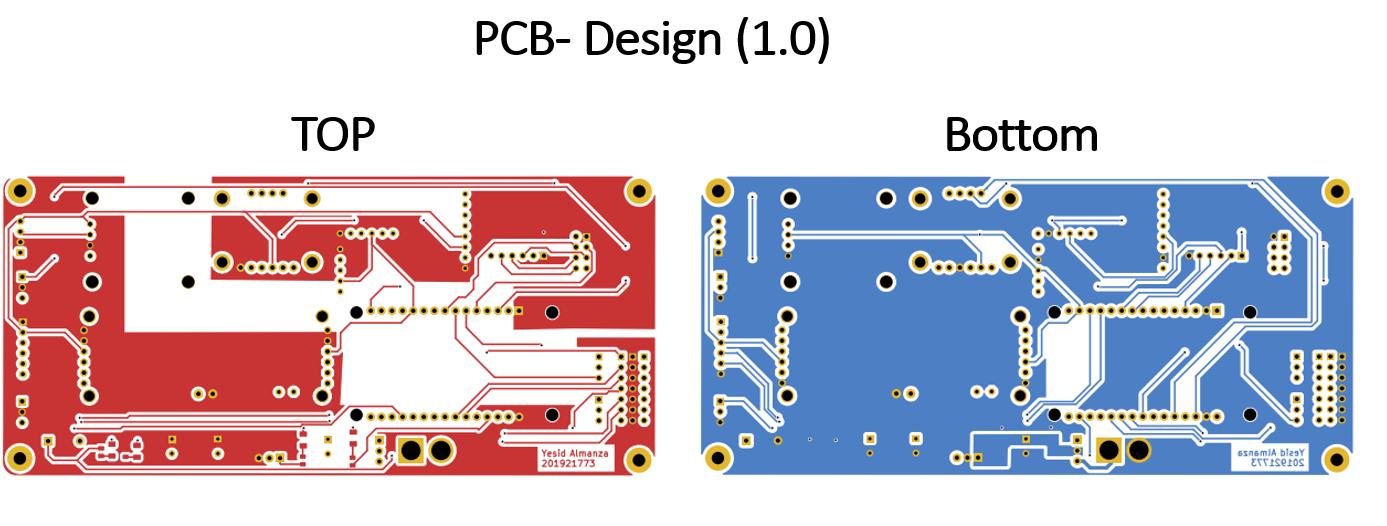
\includegraphics[width=\textwidth]{Imagenes/Anexos/layout_pcb.png}
    \caption{Layout Circuito Impreso 1.0 }
    \label{fig:pcb-1.0}
\end{figure}

\begin{figure}[H]
    \centering
    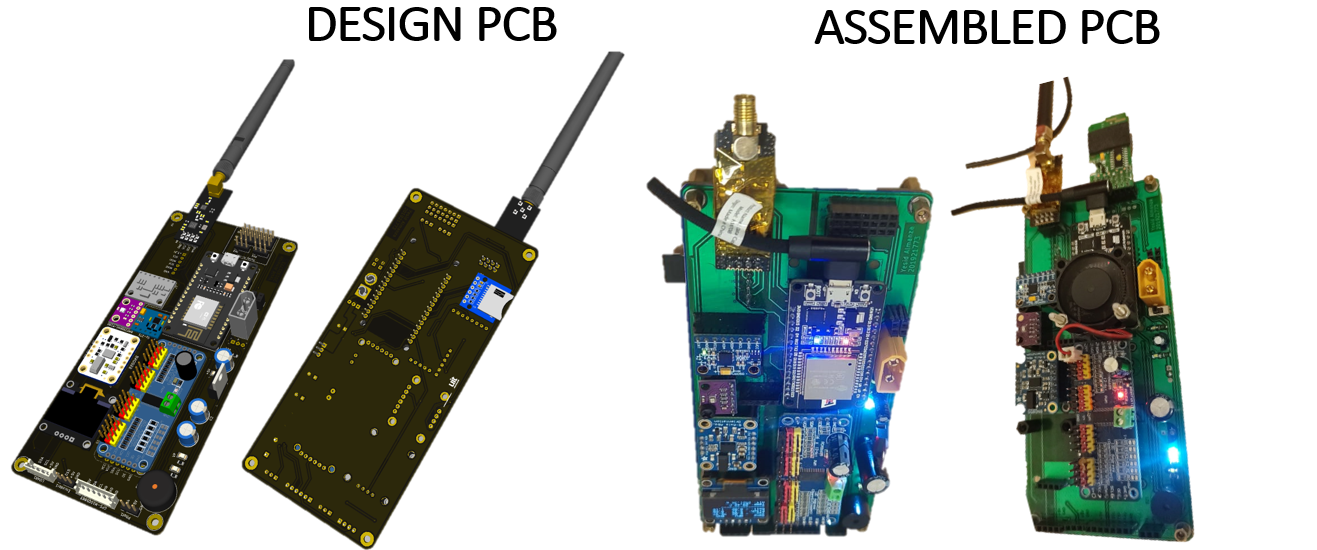
\includegraphics[width=\textwidth]{Imagenes/Anexos/pcb_primera_iteracion.png}
    \caption{Circuito Impreso Ensamblado 1.0 }
    \label{fig:pcb-ensambled-1.0}
\end{figure}

\begin{figure}[H]
    \centering
    \includegraphics[width=(\textwidth-2)]{Imagenes/Anexos/carcasa_version.png}
    \caption{Carcasas Versiones }
    \label{fig:carcasasVersion}
\end{figure}


\begin{comment}
 sdfsd
\end{comment}

\printbibliography

\end{document}